\documentclass[12pt,a4paper,twosides]{book}
\usepackage[utf8]{inputenc}
\usepackage[T1]{fontenc}
\usepackage{newpxtext,newpxmath} % quite nice, math is clear too
%\usepackage{baskervald}% Quite nice, math is the default math font.
%\usepackage{cmbright}	% sans-serif font, modernised clear math, rather broad
%\usepackage{antpolt} 	% quite nice, but rather compact
\usepackage{amsmath}
\usepackage{amsfonts}
\usepackage{amssymb}
\usepackage{physics}
\usepackage{mathtools}
\usepackage{bm}
\usepackage{bbm}
\usepackage{bbold}
\usepackage{pdfpages}
\usepackage[square,comma,numbers,super]{natbib}
\usepackage{hyperref,hypertoc,hypernat}
\usepackage{lettrine}
\usepackage{epigraph}
\usepackage{graphicx,type1cm,Zallman}\graphicspath{{figures/}}
\usepackage{bibunits}

%\renewcommand\LettrineFontHook{\Zallmanfamily}
\renewcommand{\vec}[1]{\bm{\mathrm{#1}}}
\newcommand{\unit}[1]{\,\mathrm{#1}}
\newcommand{\diff}[1]{\,\mathrm{d}{\vec{#1}}}

\begin{document}

\frontmatter
	\addtocontents{toc}{~\hfill\textbf{Page}\par}
%\addcontentsline{toc}{chapter}{Title page}
\title{\headlinefont\fontsize{35}{40}\selectfont{Ultrafast Quantum Dynamics\\\vspace{10pt}of\\\vspace{10pt}Doped\\Superfluid Helium Nanodroplets\vspace{5ex}}}
\author{\bf\color{activeColor}{Fran\c{c}ois M.G.J. Coppens}\vspace{10ex}\\Submitted: \bf{April 2018}\\ Defended: \bf{June 2018}}
\date{}
\maketitle

\clearpage{\pagestyle{empty}\cleardoublepage}	
	\cleardoublepage
	\chapter{Acknowledgements}
	We would like to thank Antonio Mu\~noz, Jordi Ort\'{\i}n, Humphrey Maris and Andrey Vilesov for useful discussions and exchanges.
	
	We would also like to thank Nicolas Renon and Emmanuel Courcelle of CALMIP who greatly improved the performance of our code.
	
	This work has been performed under Grants No. FIS2014-52285-C2-1-P from DGI, Spain, and  2014SGR401 from Generalitat de Catalunya.
	
	Manuel Barranco thanks the Universit\'e F\'ed\'erale Toulouse Midi-Pyr\'en\'ees for financial support through the ``Chaires d'Attractivit\'e 2014'' Programme IMDYNHE.
	
	The dynamic simulations presented in this work have been carried out thanks to the HPC resources of CALMIP supercomputing center (Grant P1039).
	\cleardoublepage
	\addcontentsline{toc}{chapter}{Table of Contents}
\tableofcontents
	\cleardoublepage
	\addcontentsline{toc}{chapter}{List of Publications}
\begin{bibunit}[apsrev]
	\renewcommand*\bibname{List of Publications}
	\makeatletter
	\renewcommand\@biblabel[1]{}
	\makeatother 
	\nocite{*}
	\putbib[own_publications]
\end{bibunit}
	\cleardoublepage

\mainmatter
	\chapter{Introduction}
	Superfluids are liquids and gases with remarkable properties. In particular, superfluid helium can flow through a capillary without friction due to its extremely small viscosity (at least 1500 times smaller than normal liquid helium\citep{Kapitza1938}), or creep up the wall of a container, seemingly defying the force of gravity\citep{Rollin1939} (``Rollin creeping''). Its thermal conductivity is about $3\times10^6$ times higher than that of liquid helium I or about 200 times higher than that of copper at room temperature\citep{Keesom1936}. It therefore earned the title of ``best heat conducting substance we know'' by Willem and his daughter Anna Keesom and dubbed ``\emph{supra-heat-conducting}''\citep{Keesom1936}. Later it was understood why\citep{Tisza1938-1,Tisza1938-2,Tisza1940-1,Tisza1940-2} and it turns out that heat doesn't diffuse through the medium as in normal liquids, but rather it travels through the medium in waves (second sound). This makes it an ideal coolant e.g. to stabilise the superconducting magnets in CERN's Large Hadron Collider\citep{Lebrun1994}. Helium is also the only known substance that stays liquid at zero temperature and low pressures and both its angular momentum and vorticity are quantised, making it the first observed macroscopic quantum substance. Helium-4 becomes superfluid below the $\lambda$-point, named so by William H. Keesom in 1936 who measured a singularity in the specific heat at $T_\lambda=2.2\unit{K}$\citep{Keesom1936}.
	
	\begin{figure}[t]
		\begin{center}
			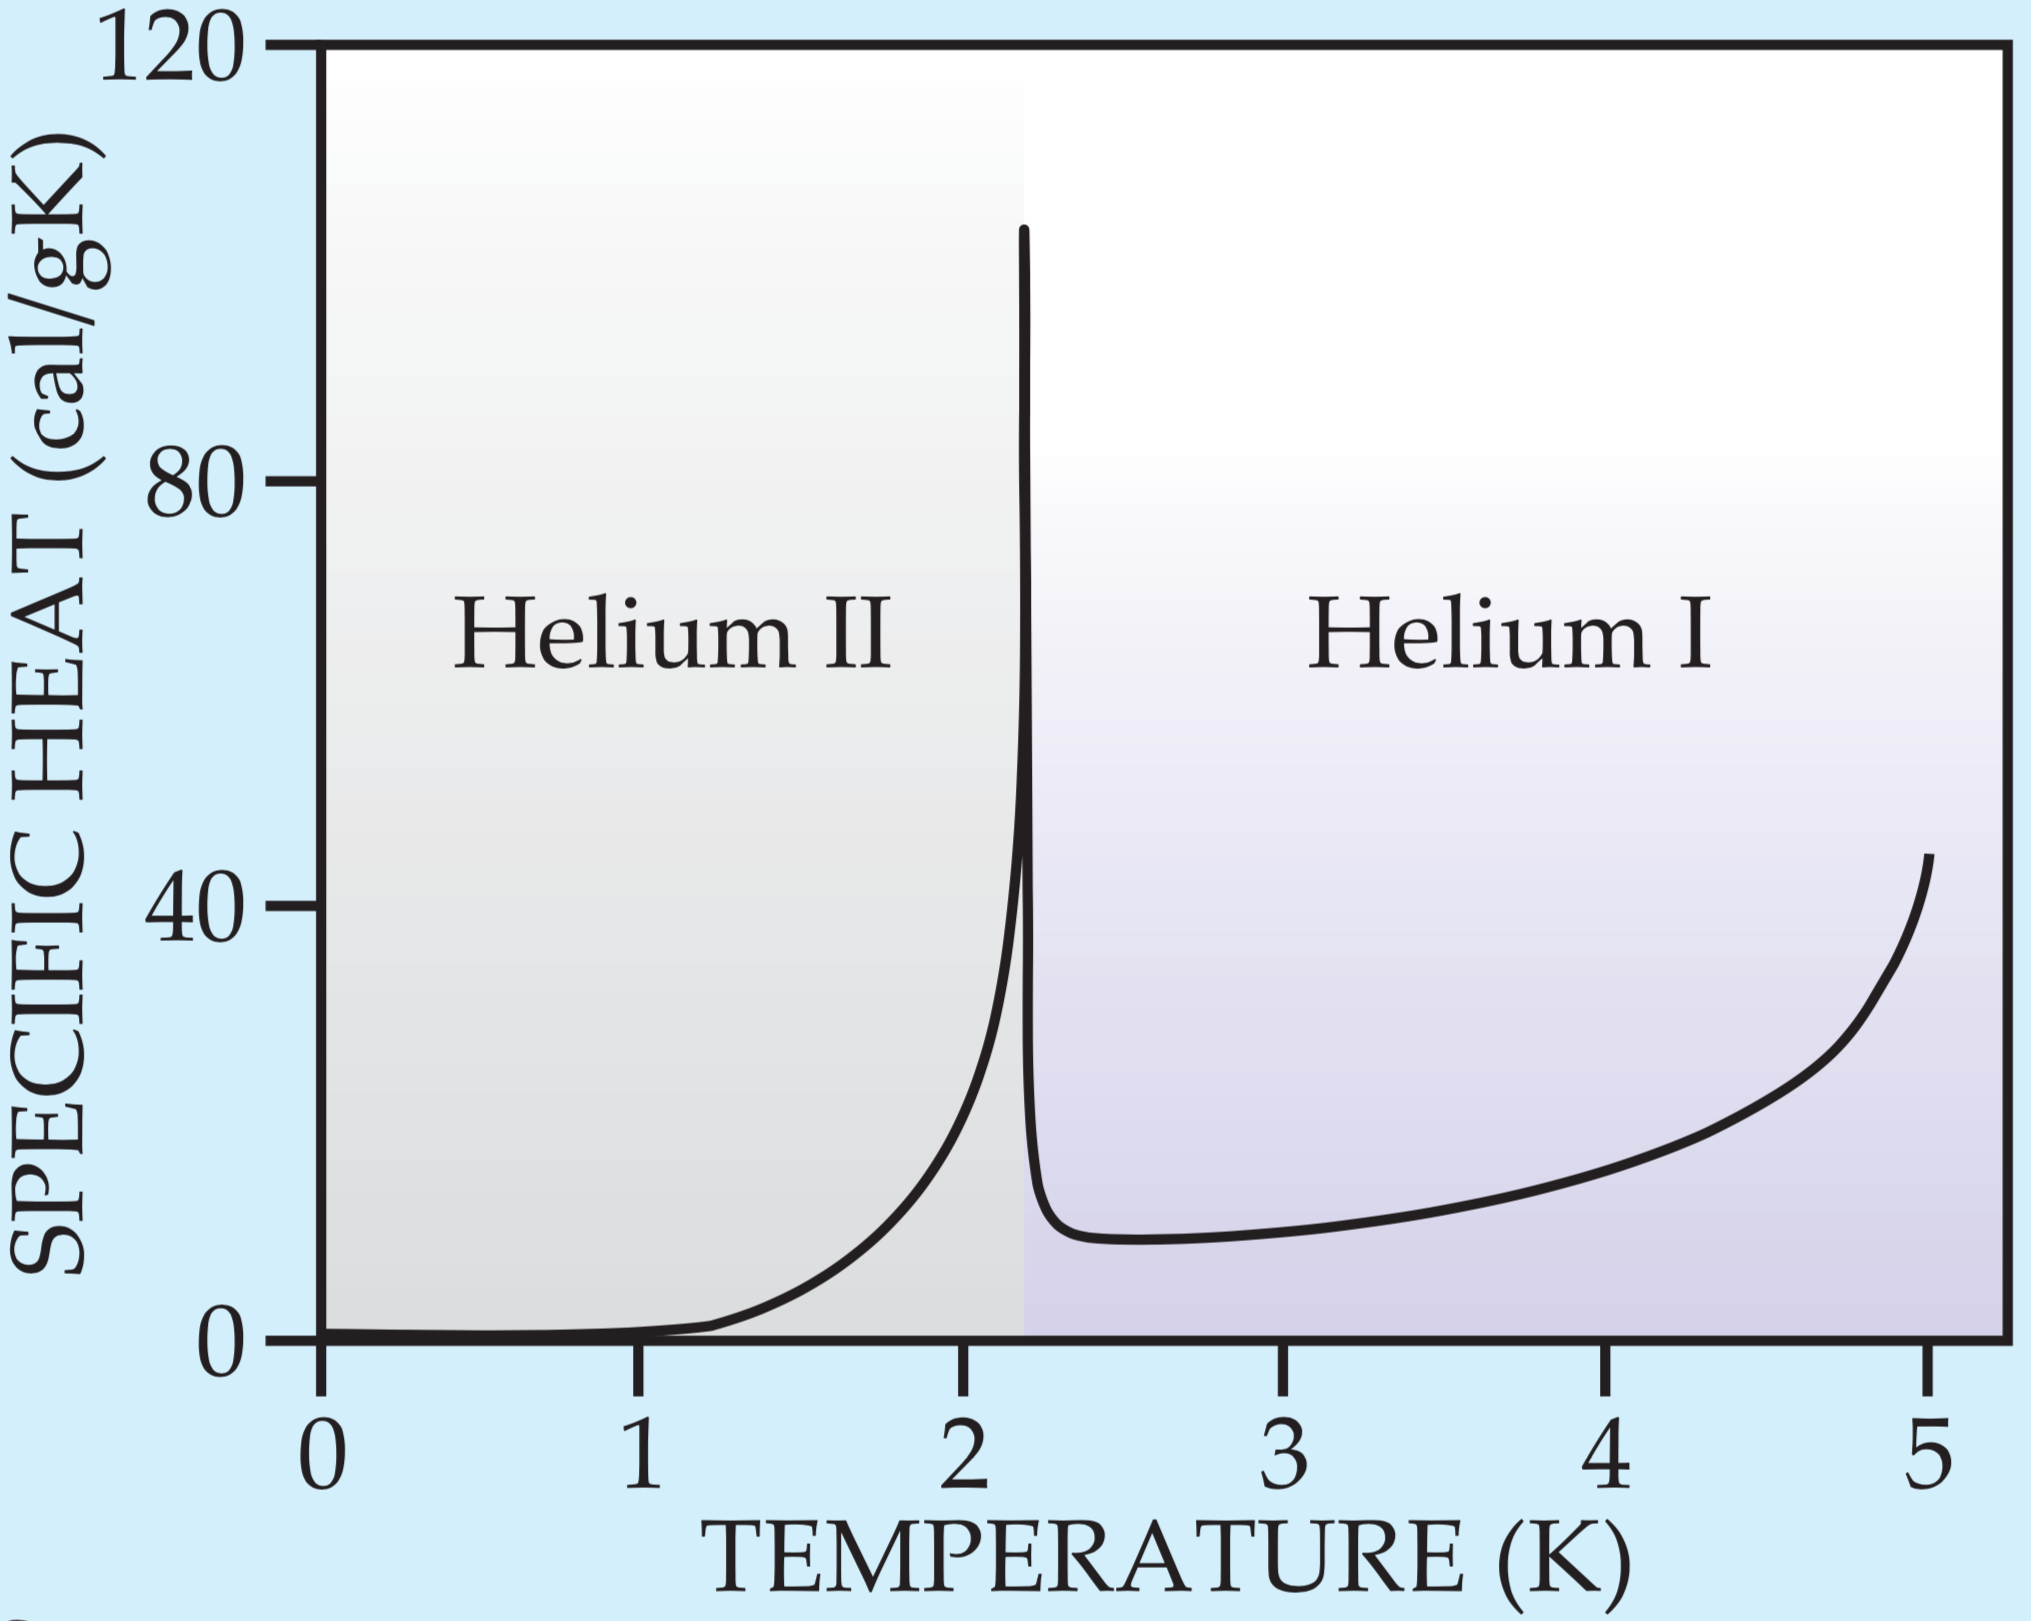
\includegraphics[width=0.75\textwidth]{specific-heat}
		\end{center}
		\caption{The specific heat of $^4$He as a function of the temperature. There is a clearly visible singularity around $2.2\unit{K}$ and the graph itself has the distinct $\lambda$-like shape that inspired\citep{Keesom1932} Willem and Anna Keesom to call the temperature at which the singularity occurs the ``$\lambda$-point''. (Illustration courtesy of R.J. Donnelly\citep{Donnelly2009})}
		\label{fig:specific-heat}
	\end{figure}	
	
	\section{A brief history of superfluidity}
		\lettrine[lines=3,findent=3pt,nindent=0pt]{H}{elium} was the last gas to be liquefied and was done so by Heike Kamerlingh Onnes in 1908\citep{Onnes1908,Onnes1909}. In 1932 John McLennan saw that liquid helium stopped boiling below $\approx\!2.2\unit{K}$\citep{McLennan1932} and later that year Willem Keesom and his daughter Anna observed, while measuring the temperature dependence of the specific heat, a singularity around the same temperature\citep{Keesom1932}. They called it the ``$\lambda$-temperature'',  $T_\lambda$, because of the shape of the temperature dependence of the specific heat resembling the Greek letter $\lambda$ (see Figure \ref{fig:specific-heat}). A few years later in 1935 Burton measured a sharp decrease in the viscosity of liquid helium below $T_\lambda$\citep{Burton1935}. Around the same time Fritz London was already thinking about macroscopic wave functions and why helium does not freeze at $T=0\unit{K}$ under atmospheric pressure\citep{London1935}. London and Simon concluded that it was caused by the zero point motion of the helium atoms and their associated kinetic energy that is comparable to their Van der Waals energy, effectively preventing liquid helium to solidify\citep{Simon1934,London1936}. The year after, in 1936, Willem and Anna Keesom measured an abnormally high heat conductance below $T_\lambda$\citep{Keesom1936}. This was confirmed roughly one year later by J.F. Allen \emph{et al.}\citep{Allen1937} and it was understood that the high thermal conductance was the reason for the helium to stop boiling whenever the temperature drops below $T_\lambda$. It was in 1937, when Kapitza tried to determine the viscosity of the laminar flow, that he measured a viscosity that was about $10^4$ times smaller than that of hydrogen gas\citep{Kapitza1938}. It was then that Kaptiza who, by analogy with superconductors, first coined the word ``superfluid''\citep{Kapitza1938} to describe the special state that helium enters below the $\lambda$-point where it can flow, seemingly without friction. Allen and Misener realised that superfluid helium is not just a liquid with a very low viscosity, but that its hydrodynamics was completely different from that of ordinary liquids\citep{Allen1938} and therefore required a completely new interpretation.\\
		
		The start of this new interpretation was made by London\citep{London1938} in 1938 when he made a connection between the behaviour of superfluid helium and that of an ideal ``Bose-Einstein'' (BE) gas. Both his calculated value for $T_c=3.09\unit{K}$ and the behaviour of the temperature dependence of the heat capacity for the ideal BE-gas were very similar to the measured ones for liquid helium below $T_\lambda$. He wrote to Nature that ``it was difficult not to imagine a connection with ``Bose-Einstein condensation'' (BEC). Tisza expanded upon London's ideas\citep{Tisza1938} and considered a Helium II system of total $N$ atoms to consist of two parts; a macroscopic ``condensed'' part $n_0$, the superfluid component, in the ground state, and the remaining part $n=N-n_0$, the normal component, where the helium atoms are distributed over the excited states. Assuming this was correct the fraction $n_0/N$ should decrease with increasing temperature according to the equation\\
		\begin{align}
			\frac{n_0}{N} = 1-\qty(\frac{T}{T_0})^s \quad \text{for} \quad T<T_0
		\end{align}
		where $s=3/2$ for an ideal gas and should be taken larger, e.g. $s=5$, for a real liquid with stronger interactions between the atoms.\\
		
		This was the birth of the ``two-fluid'' model. With this model he derived two hydrodynamic equations for liquid helium below $T_\lambda$ and discovered that within it, heat propagates in waves instead of diffusing through the medium, and calculated the velocity of these waves. He also explained why the viscosity is disappearing at low temperatures contrary to classical liquids where the viscosity increases\citep{Tisza1938-1,Tisza1938-2,Tisza1940-1,Tisza1940-2}. In 1941 Lev Landau reformulated Tisza's theory on a more rigorous footing\citep{Landau1941,Landau1949}. He assumed, contrary to Tisza, that the normal component of the liquid was made-up of collective excitations instead of excited single atoms. He postulated that the liquid could exhibit two states of motion which he called ``potential motion'' that is irrotational ($\curl{\vec{v}}=0$), and ``vortex motion'' that is rotational ($\curl{\vec{v}} \neq 0$). The corresponding energies of these two motions are discontinuously separated by an energy gap $\Delta$. In case of potential internal motion  the excitations are quanta of longitudinal (sound) waves, i.e., phonons. The excitations of the vortex-spectrum could be called ``rotons'' (see Figure \ref{fig:phonon-roton}).\\

		\begin{figure}[t]
			\begin{center}
				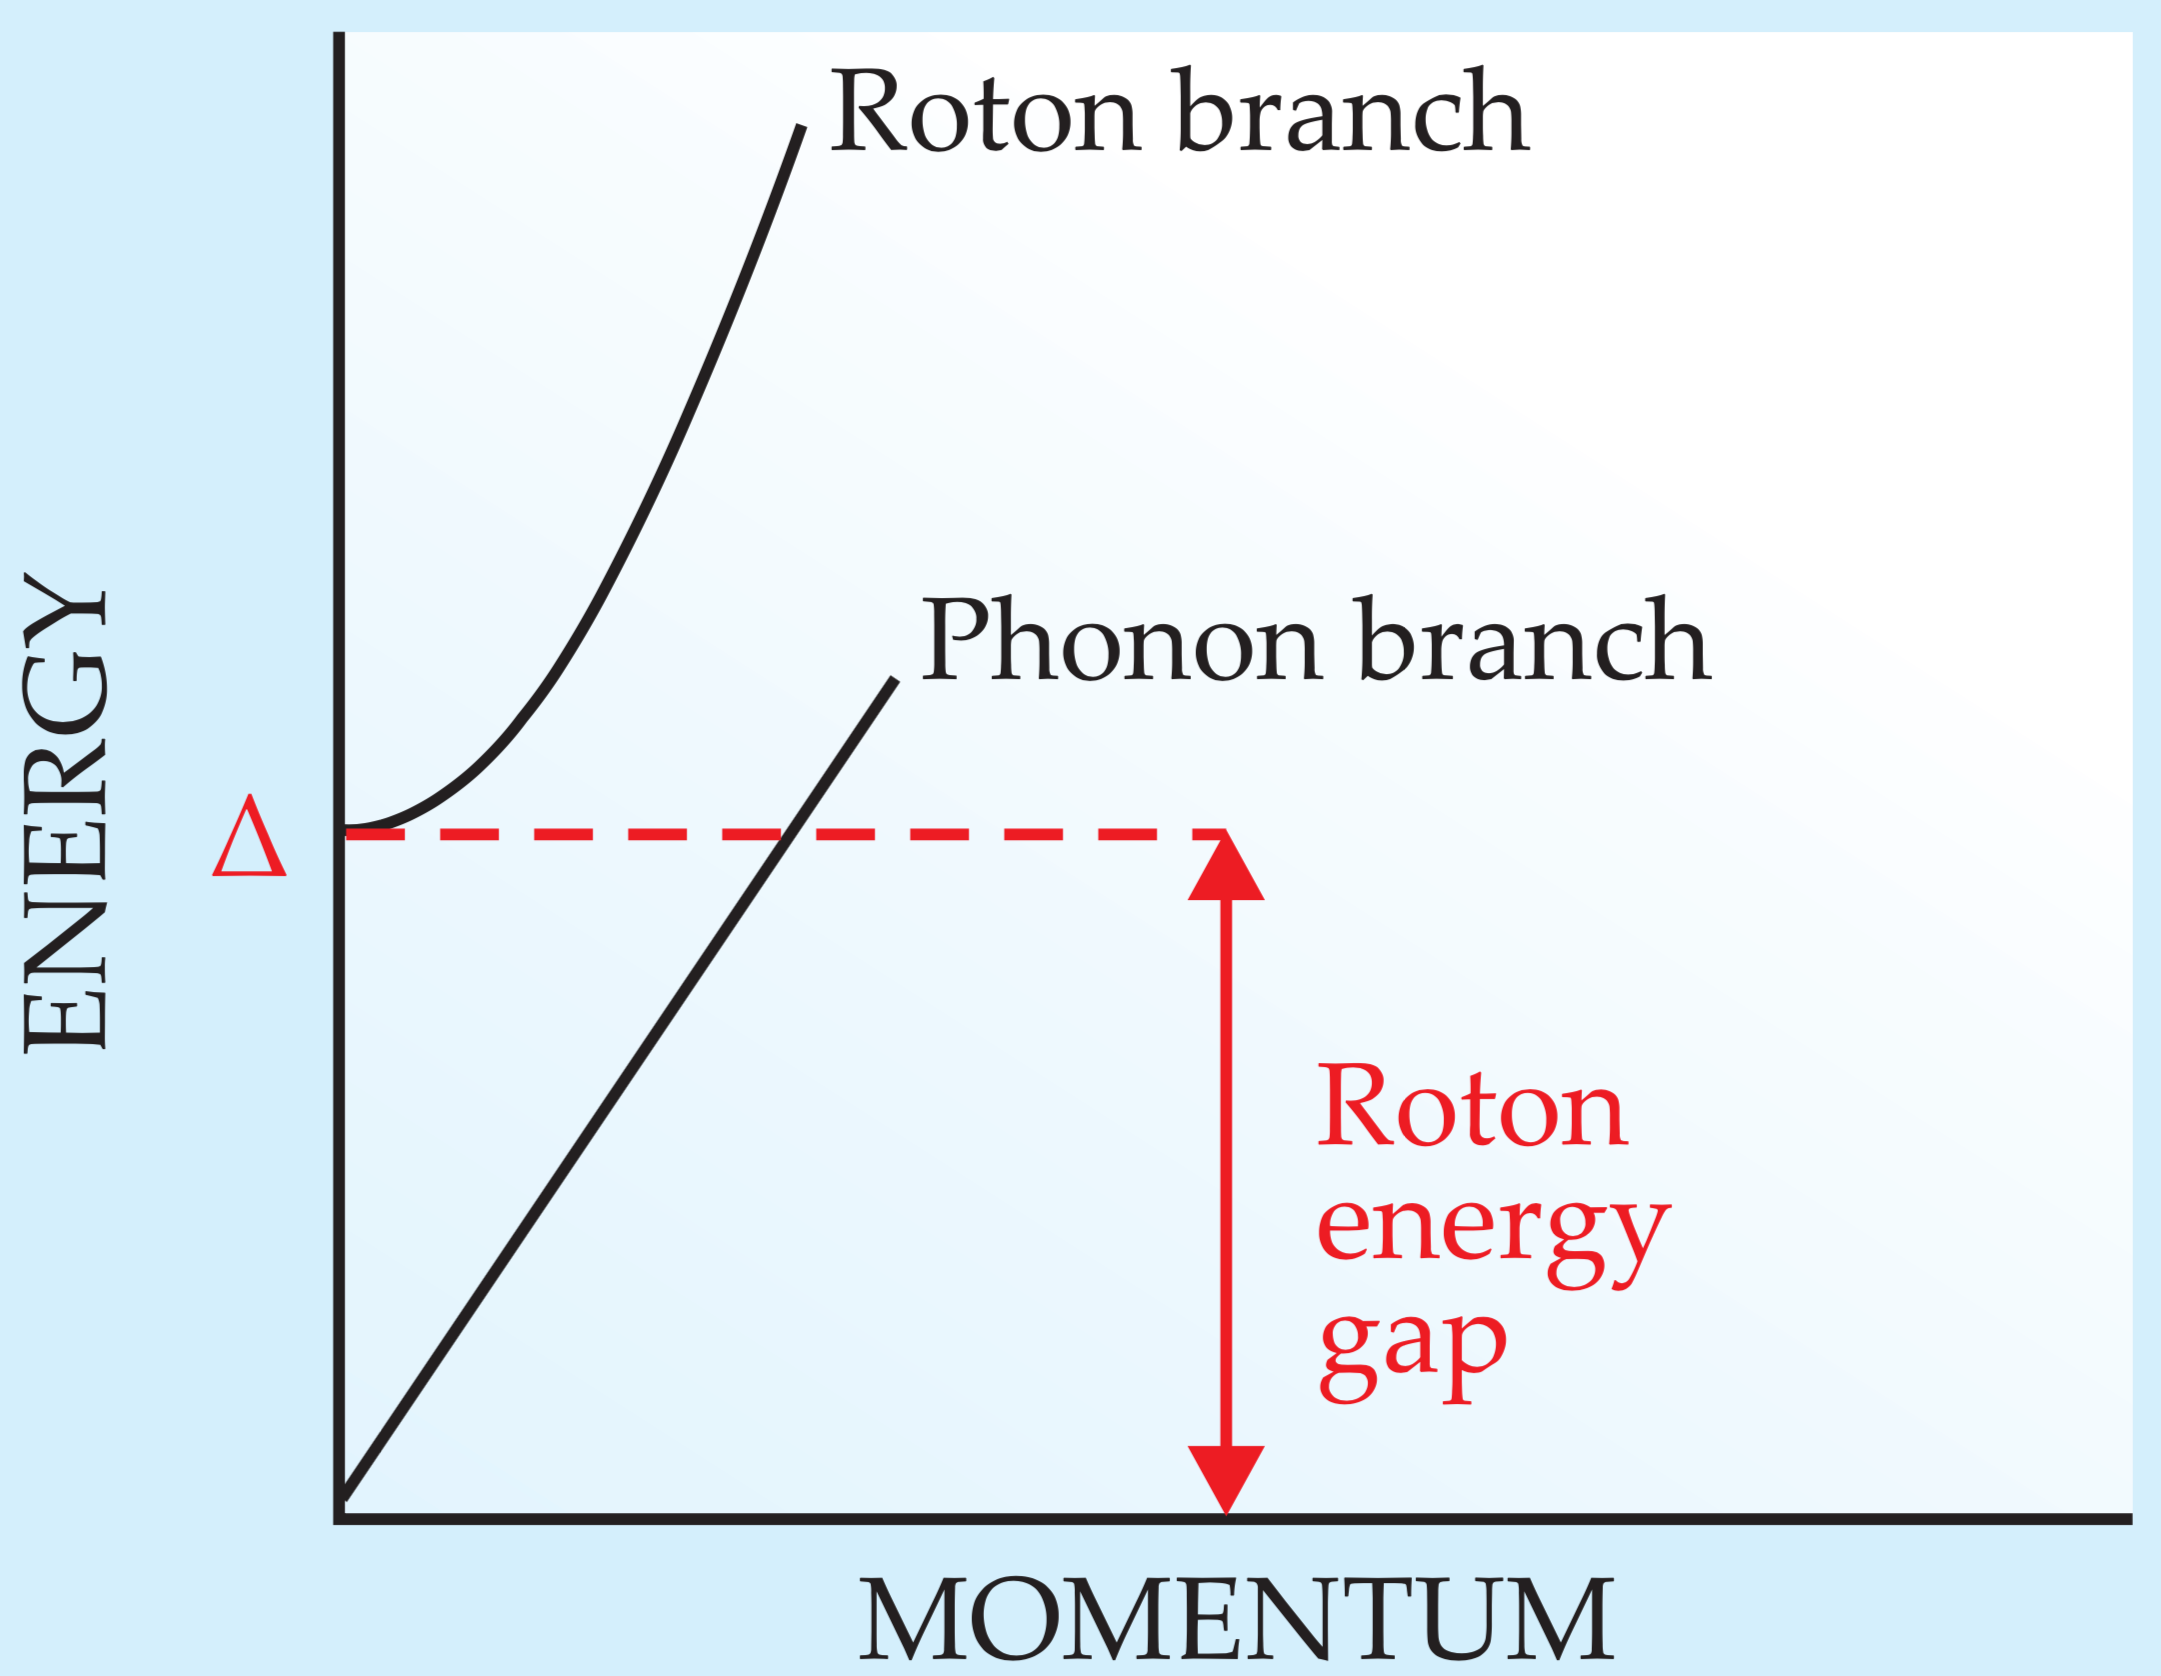
\includegraphics[width=0.495\textwidth]{phonon-roton-landau-first}
				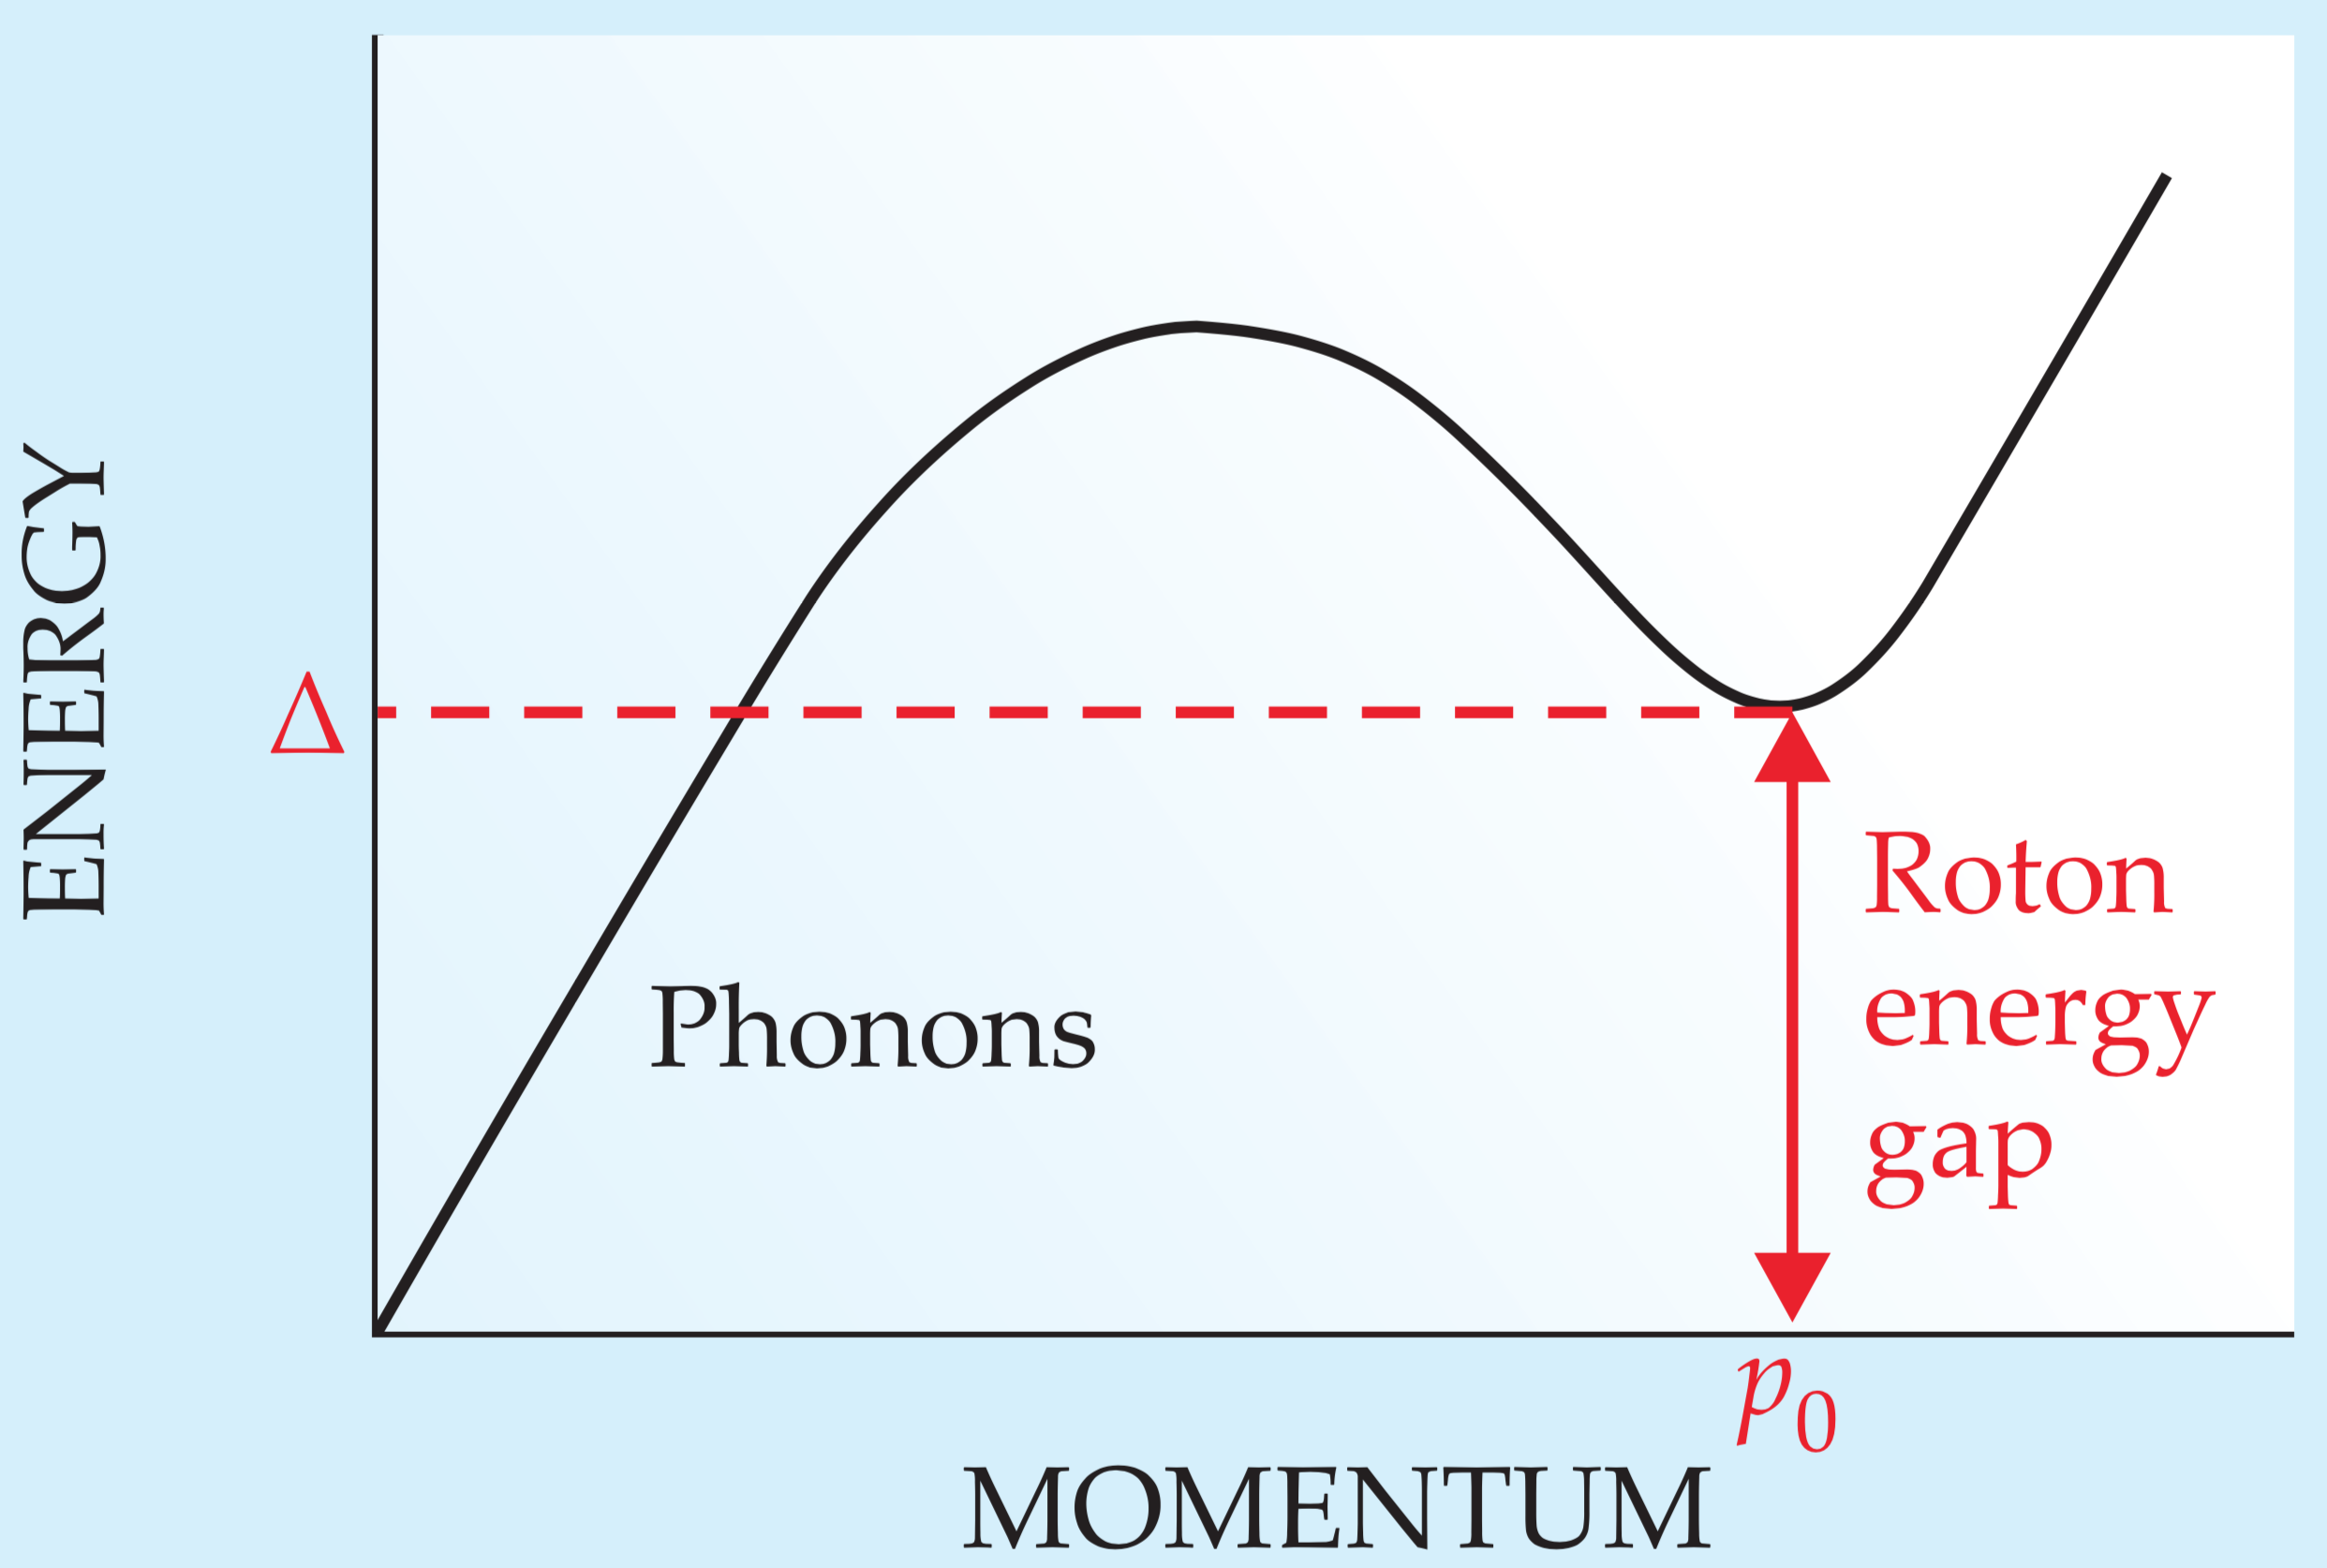
\includegraphics[width=0.495\textwidth]{phonon-roton-bogoliubov}
			\end{center}
			\caption{Left: Lev Landau's 1941 energy dispersion curve\citep{Landau1941} for the excitations in liquid helium below $T_\lambda$. It exhibits a phonon- and a roton branch. The slope of the linear phonon branch corresponds to the velocity of sound. Right: Lev Landau's 1947 modified dispersion curve. The roton-branch is no longer a separate excitation branch but rather an extension of the phonon-branch. (Illustration courtesy of R.J. Donnelly\citep{Donnelly2009})}
			\label{fig:phonon-roton}
		\end{figure}

		A theoretical demonstration, explicitly showing that phonons and rotons are collective excitations of the liquid, came in the form of a 1947 paper by Nikolay Bogolyubov\citep{Bogolyubov1947}. The intimate relationship between superfluidity and BEC was not universally accepted until 1995 when Cornell and Wienman in Colorado and Ketterle at MIT discovered BEC in rubidium quantum gases\citep{Cornell2002,Ketterle2002}.

	\section{Some key concepts}
		\lettrine[lines=3,findent=3pt,nindent=0pt]{I}{n} this section I will briefly introduce some key ideas that are used throughout the thesis and that are needed to fully appreciate the discussed material. Also references to more complete and more in-depth treatments will be provided for the interested reader.
		
		\subsection{Bose-Einstein condensation and long-range order}
			The essential concept of Bose-Einstein (BE) condensation is the fact that at low temperatures, multiple bosons, unlike fermions, will occupy the same quantum state. In theory there is no upper bound of how many bosons can occupy such a single state. It is then said that, with ever decreasing temperature, a macroscopic part of the total number of bosons will ``condense'' into the quantum state with the lowest energy.\\			
			
			Another important concept in BEC is the idea of long-range order. Let us start by introducing the one-body density matrix of a system of $N$ bosons in a pure state $\Psi_k(\vec{r}_1,\vec{r}_2,\ldots,\vec{r}_N)$
			\begin{align}
				n^{(1)}_k(\vec{r},\vec{r'}) \vcentcolon= N\int\!	\Psi_k^*(\vec{r},\vec{r}_2,\ldots,\vec{r}_N)\Psi_k(\vec{r'},\vec{r}_2,\ldots,\vec{r}_N)\diff{r}_2\diff{r}_3\ldots\diff{r}_N	\label{eq:def-obd-matrix}
			\end{align}
			where the integral is taken over the $N-1$ coordinates $\vec{r}_2,\vec{r}_3,\ldots,\vec{r}_N$. For a statistical mixture of quantum states one needs to take the weighted average over all the different $\Psi_k$-states. In thermodynamic equilibrium the states are Boltzmann weighted by their eigenvalues $\qty{E_k}$
			\begin{align}
				n^{(1)}(\vec{r},\vec{r'}) = \frac{1}{Q}\sum_k n^{(1)}_k(\vec{r},\vec{r'}) \unit{e}^{-E_k/k_BT}
			\end{align}
			where $Q$ is the partition function. For more general cases the one-body density matrix is defined
			\begin{align}
				n^{(1)}(\vec{r},\vec{r'}) \vcentcolon=\expval{\hat\Psi^\dagger(\vec{r})\hat\Psi(\vec{r'})}
			\end{align}
			where $\hat\Psi^\dagger(\vec{r})$/$\hat\Psi(\vec{r})$ are field-operators creating/annihilating a boson at $\vec{r}$ and the averaging $\expval{\cdots}$ is taken over all states in the mixture. Once it is accepted that a macroscopic part of the total number of bosons can occupy a single quantum state it can be demonstrated that, while considering a uniform isotropic sytem of $N$ bosons, the one-body density matrix (Eq. \ref{eq:def-obd-matrix}) tends to a constant value when the distance between $\vec{r}$ and $\vec{r}'$ goes to infinity. In the thermodynamic limit where $N,V\rightarrow\infty$ such that $n=N/V$ is kept fixed, the one-body density only depends on the modulus of the relative variable $\vec{s}:=\vec{r}-\vec{r}'$ so that we can write it as the Fourier transform of the momentum distribution as
			\begin{align}
				n^{(1)}(s) = \frac{1}{V}\int \! n^{(1)}\qty(\vec{p})\exp(i\vec{p}\cdot\vec{s}/\hbar)\,\mathrm{d}\vec{p} \label{eq:one-body-den-mom}
			\end{align}
			For a BEC system, the momentum distribution at small momenta is not smooth but has a sharp peak around $p=0$ for the bosons that are in the ground state, while the remaining bosons are smoothly distributed over the excited states.
			\begin{align}
				n(\vec{p})=N_0\delta(\vec{p})+\tilde{n}(\vec{p})
			\end{align}
			where $\tilde{n}$ is a smoothly varying function of $\vec{p}$. When this expression is plugged into Eq. (\ref{eq:one-body-den-mom}) and taking the limit where $s$ goes to infinity
			\begin{align}
				\lim_{s\rightarrow\infty}n^{(1)}(s)=\frac{N_0}{V},
			\end{align}
			where $N_0/V \vcentcolon= n_0\leq 1$ is called the condensate fraction. It is called long-range order since it involves the off-diagonal elements of the one-body density matrix; the elements that are usually associated with the coherences.\\
			
			A set of eigenvalues \{$n_i$\} of the one-body density matrix can be defined through the following eigenvalue equation
			\begin{align}
				\int \! n^{(1)}(\vec{r},\vec{r'})\varphi_i(\vec{r'}) \,\mathrm{d}\vec{r'} = n_i\varphi_i(\vec{r})
			\end{align}
			and its solutions \{$\varphi_i$\} form a natural orthonormal basis set of single boson wave functions $\int\!\varphi_i^*\varphi_j\,\mathrm{d}\vec{r}=\delta_{ij}$, with normalisation condition $\sum_i n_i=N$. This permits writing the on-body density matrix in a useful diagonalised form and recalling that BEC occurs when a single particle state $\varphi_i$ is occupied in a macroscopic way, say when $n_{i=0}=N_0$, a number of order $N$, we separate the condensate part from the rest
			\begin{align}
				n^{(1)}(\vec{r},\vec{r'}) = N_0\varphi_0^*(\vec{r})\varphi_0(\vec{r'})+\sum_{i\neq0}n_i\varphi_i^*(\vec{r})\varphi_i(\vec{r'}) \label{eq:obdm-diag}
			\end{align}

		\subsection{Bogolyubov's approximation and the order parameter}\label{sec:bogol-order}
			It is customary, given the importance of the condensate fraction $N_0$ in a BEC, to write the field operator of a $N$-body boson system as the sum of the condensate part and the rest, just as the one-body density matrix
			\begin{align}
				\hat{\Psi}(\vec{r})=\varphi_0(\vec{r})\hat{a}_0 + \sum_{i\neq 0} \varphi_i(\vec{r})\hat{a}_i \label{eq:field-operator}
			\end{align}
			where the $\hat{a}_i$ and $\hat{a}_i^\dagger$ are annihilation and creation operator of a particle in state $\varphi_i$ and obey the usual bosonic commutation relations
			\begin{align}
				\commutator{\hat{a}_i}{\hat{a}_j^\dagger}=\delta_{ij},\quad 	\commutator{\hat{a}_i}{\hat{a}_j}=0=\commutator{\hat{a}_i^\dagger}{\hat{a}_j^\dagger}
			\end{align}
			Using Eq. (\ref{eq:field-operator}) in Eq. (\ref{eq:def-obd-matrix}) and comparing it to Eq. (\ref{eq:obdm-diag}) one finds the expectation value of $\expectationvalue{\hat{a}_j^\dagger\,\hat{a}_i}=\delta_{ij}n_i$. Now, the Bogolyubov approximation essentially replaces the operators $\hat{a}_0$ and $\hat{a}_0^\dagger$ with the $c$-number\footnote{The term $c$-number is old nomenclature for a classical number, which can be real or complex, to distinguish them from quantum numbers, or $q$-numbers, that are represented by operators.} $\sqrt{N_0}$. This is equivalent to ignoring the non-commutative nature of the operators due to the macroscopic occupation of the state $\varphi_0$, when $N_0=\expectationvalue{\hat{a}_0^\dagger\,\hat{a}_0}\gg 1$. We then rewrite the field operator as the sum of a classical field for the condensed component and quantum field for the non-condensed component
			\begin{align}
				\hat{\Psi}(\vec{r})=\Psi_0(\vec{r})+\delta\hat{\Psi}(\vec{r}),\label{eq:order-param-real}
			\end{align}
			where $\delta\hat{\Psi}(\vec{r})=\sum_{i\neq 0}\varphi_i(\vec{r})\hat{a}_i$ and $\Psi_0(\vec{r})=\sqrt{N_0}\varphi_0(\vec{r})$. At $T=0$ the whole system is condensed and one can ignore $\delta\hat{\Psi}$ altogether; the field operator becomes a normal function of space $\Psi_0$.\\
			
			The classical field $\Psi_0$ is called the \emph{effective}- or \emph{macroscopic} wave function of the condensate and it behaves like an order parameter in the sense that it varies continuously between a maximum value $\sqrt{N}$, that is proportional to the total number particles in the system, at $T=0$, and vanishes at the superfluid-normal fluid phase transition temperature $T_\lambda$. It is a complex quantity characterised by a real-valued modulus and phase $S$:
			\begin{align}
				\Psi_0(\vec{r}) = \absolutevalue{\sqrt{N_0}\varphi_0(\vec{r)}}\,\mathrm{e}^{iS(\vec{r})}\label{eq:order-param-complex}
			\end{align}
			The modulus determines the number-density of the condensate, while the phase $S$ plays an important role in the coherence and properties of the superfluid. As we will see in Section \ref{sec:rot-vort}, $S$ plays the role of a velocity potential.\\
			
			Using an order parameter as defined here is equivalent to using the many-body wave function
			\begin{align}
				\Phi(\vec{r}_1,\vec{r}_2,\ldots\vec{r}_N)=\prod_{i=1}^{N}\varphi_0(\vec{r}_i),
			\end{align}
			with a density operator $\hat{\rho}(\vec{r}) \vcentcolon= \sum_{i=1}^{N}\delta(\vec{r}-\vec{r}_i)$ (see Section \ref{sec:dft-method}). One way to see why this wave function plays the role of an order parameter is to look at its time dependence. For normal wave functions the time dependence is determined by the eigenvalues $E_i$ of the Hamiltonian of the system
			\begin{align}
				\Psi(\vec{r},t)=\psi(\vec{r})\,\mathrm{e}^{-iE_it/\hbar}
			\end{align}
			But in this case, the time dependence is determined by the chemical potential $\mu=E(N)-E(N-1)\approx \partial E/\partial N$
			\begin{align}
				\Psi_0(\vec{r},t)=\Psi_0(\vec{r})\,\mathrm{e}^{-i\mu t/\hbar} \label{eq:td-order-param}
			\end{align}
			Another aspect of $\Psi_0$ being an order parameter and not a true many-body wave function is that two solutions $\Psi_a$ and $\Psi_b$ of the non-linear droplet Hamiltonian corresponding to two different values of the chemical potential $\mu_a$ and $\mu_b$ are not necessarily orthogonal, i.e. $0 \leq N^{-1}\int\!\Psi_a^*\Psi_b\unit{d}\vec{r} < 1$. However, in dilute gases it is possible to construct a many-body wave function from the order parameter that regains its orthonormality in the thermodynamic limit
			\begin{align}
				\Phi_0(\vec{r}_1,\vec{r}_2,\ldots,\vec{r}_N) = \qty(\frac{1}{\sqrt{N}}\Psi_0(\vec{r}_1))\qty(\frac{1}{\sqrt{N}}\Psi_0(\vec{r}_2))\cdots\qty(\frac{1}{\sqrt{N}}\Psi_0(\vec{r}_N))
			\end{align}
			
		\subsection{Landau's criterion for superfluidity}
			\begin{figure}[t]
				\begin{center}
					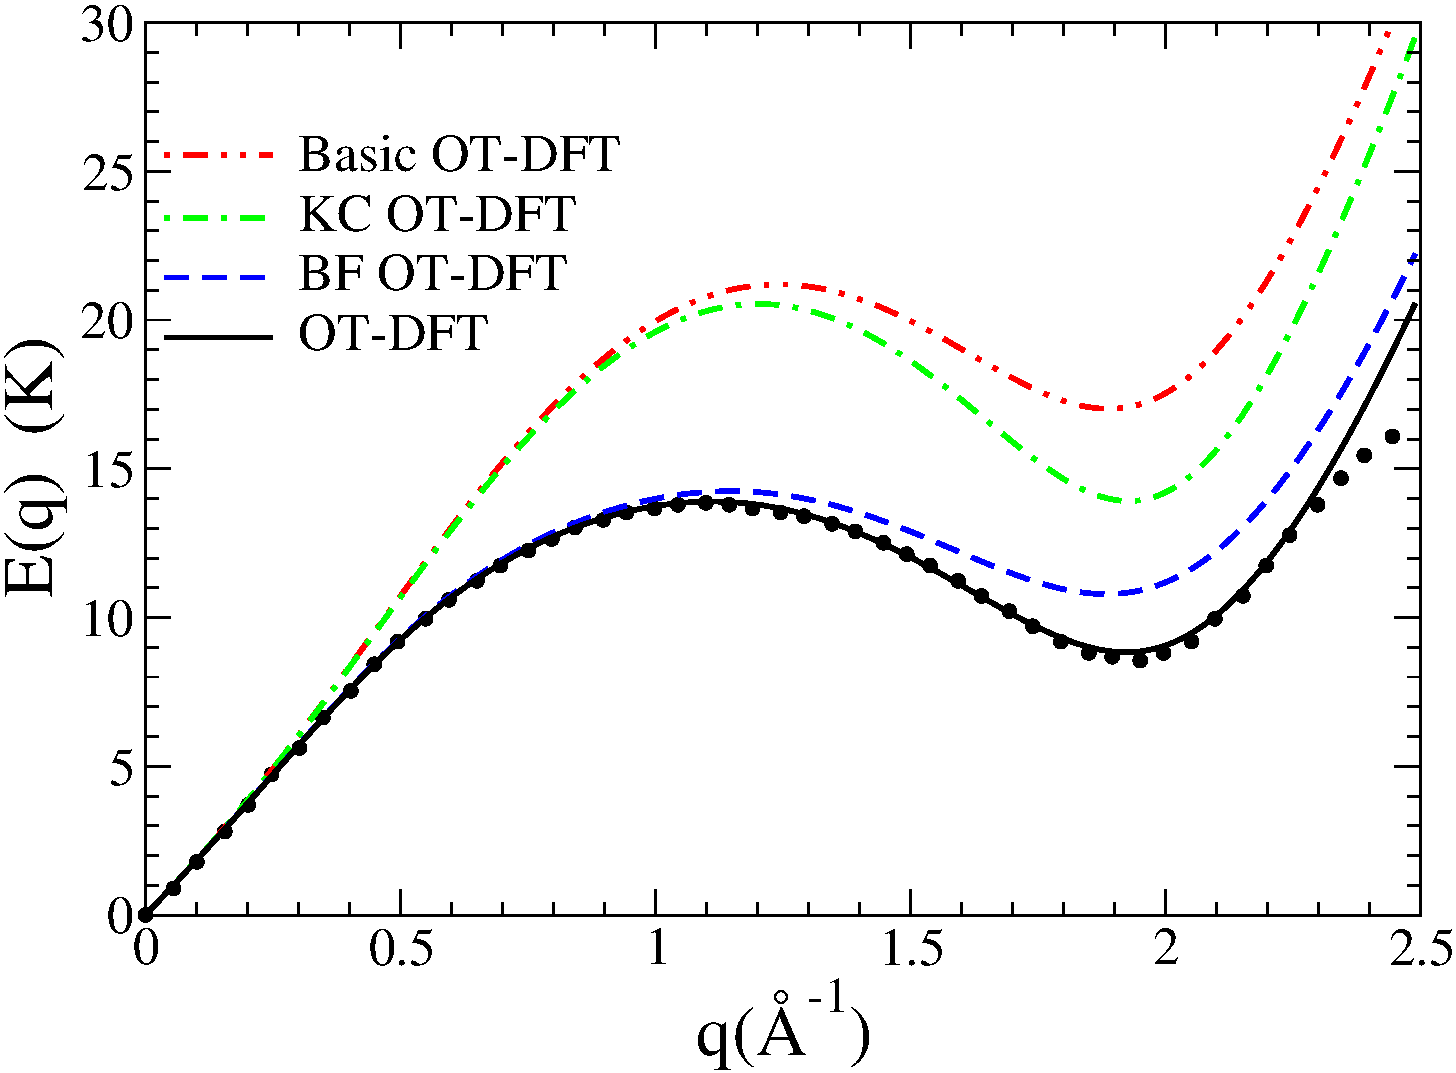
\includegraphics[width=0.9\textwidth]{dispersion-relation}
					\caption{Dispersion relation for elementary excitations in liquid $^4$He calculated as in  \cite{Mat10a}. `Basic' indicates the OT-DFT without the non-local kinetic energy correlation (KC) nor the back-flow (BF) terms; KC OT-DFT adds  to the basic OT-DFT the KC term; BF OT-DFT adds to the basic OT-DFT the BF term. The dots are the experimental data from \cite{Don81}. The Landau velocity $v_L = E(q)/(\hbar\,q)|_{min}$ obtained for each functional is  60.3 m/s (OT-DFT); 75.1 m/s (BF OT-DFT); 94.4 m/s (KC OT-DFT); 118 m/s (basic OT-DFT); and 57.5 (experiment).}
					\label{fig:dispersion-relation}
				\end{center}
			\end{figure}
		
			For a gas or liquid to be able to become superfluid Landau postulated that the energy dispersion relation needs to fulfil certain requirements. Specifically for a fluid to flow  without dissipation, i.e. a super-flow, the velocity field needs to fulfil the following inequality:
			\begin{align}
				v<v_c = \min_{\vec{p}}\frac{\epsilon(\vec{p})}{p}
			\end{align}
			
			For an ideal Bose gas $\epsilon(\vec{p})= \frac{p^2}{2m}$. In this case 
			\begin{align}
				v_c &= \min_{\vec{p}}\frac{\epsilon(\vec{p})}{p} \\
					&= \min_{\vec{p}}\frac{p}{2m} \\
					&= 0
			\end{align}
			Apparently ideal Bose-gases cannot become superfluid.\\
			
			But if we allow for some weak interactions between the bosons the energy dispersion relation is given by
			\begin{align}
				\epsilon(\vec{p})=\sqrt{\frac{gn}{m}p^2+\qty(\frac{p^2}{2m})^2},
			\end{align}
			Bogolyubov's dispersion law for elementary excitations (1947). And thus
			\begin{align}
				v_c &=\min_{\vec{p}}\sqrt{\frac{gn}{m}+\frac{p^2}{4m^2}} \\
					&= \sqrt{\frac{gn}{m}} \\
					&= c,
			\end{align}
			the speed of sound. Here $g=\frac{4\pi\hbar^2a}{m}$, and $a$ the $s$-wave scattering length. The weakly interacting Bose gases can become superfluid.\\			

			Liquid helium below the $\lambda$-point has a similar energy dispersion relation (see Figure \ref{fig:dispersion-relation}) hence reinforcing the notion that superfluidity and Bose--Einstein condensation are two intimately related concepts. The experimental value of the speed of sound is $\sim\!57.5\unit{m/s}$.
			
		\subsection{Rotation and vorticity in superfluids}\label{sec:rot-vort}
			\begin{figure}[t]
				\begin{center}
					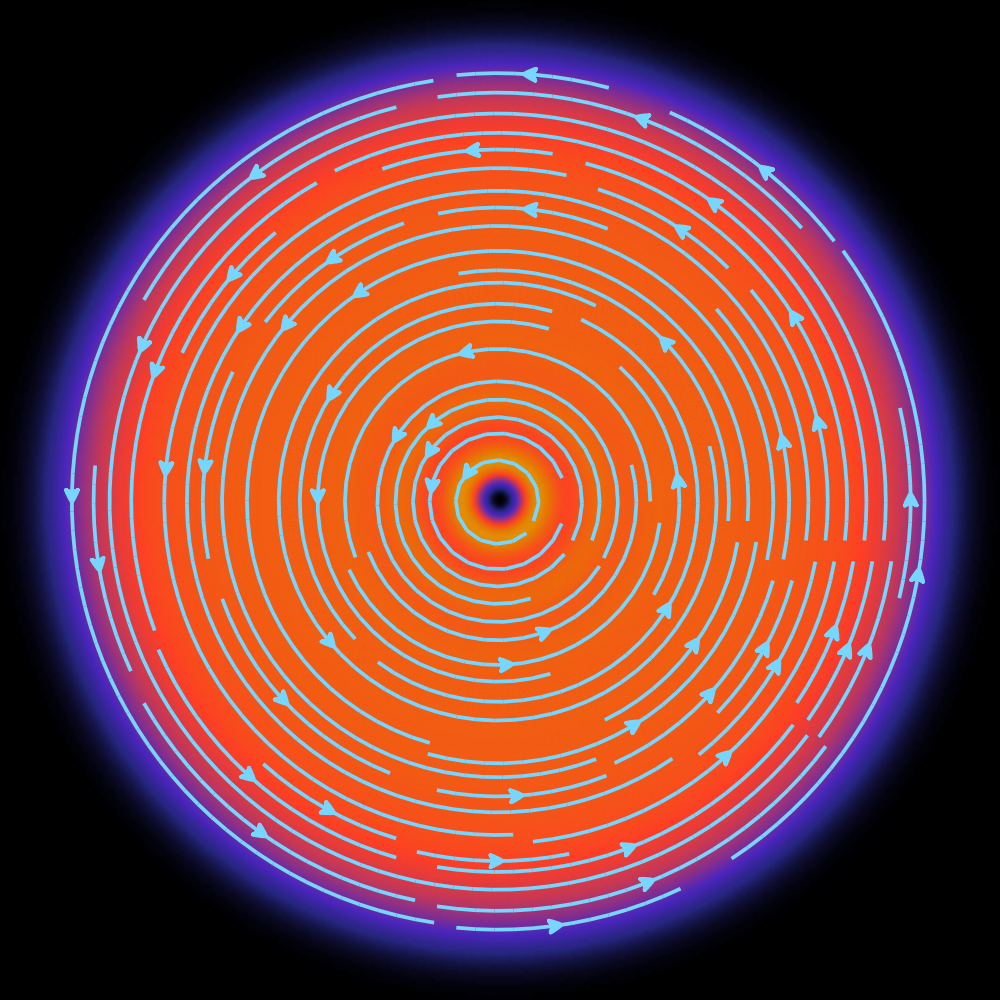
\includegraphics[width=0.5\textwidth]{vortex-xy}
					\caption{Cross section of a $^4$He droplet through a symmetry plane. The droplet is made of 1000 atoms. Superimposed in cyan are the streamlines of the velocity field $\vec{v}_s$ for $s=1$. They are concentric circles, centred around the vortex core along the $z$-axis. The colour scale encodes for the density $\rho(r)$. The radius of the droplet is about 22\,\AA.}
					\label{fig:vortex-xy}
				\end{center}
			\end{figure}
		
			Starting from time-dependent Euler-Lagrange (EL) equation (Eq. \ref{eq:td-el-equation}, see Chapter \ref{sec:dft-method}) for the time-evolution of the order parameter $\Psi$ (Eq. \ref{eq:order-param-complex}, dropping the ground-state subscript and allowing $\varphi$ and $S$ to vary in time)
			\begin{align}
				i\hbar\frac{\partial}{\partial t} \Psi({\mathbf r},t) = \left[-\frac{\hbar^2}{2m}\laplacian + \frac{\delta{\cal E}_{c}}{\delta\rho}\right]\Psi(\textbf{r},t)
			\end{align}
			one left-multiplies it with the complex conjugate of the order parameter $\Psi^*$ and then subtract the complex conjugate of the whole expression on both sides. After some algebra and defining $\rho(\vec{r},t)\vcentcolon=N\abs{\varphi(\vec{r},t)}^2$, one arrives at the continuity equation
			\begin{align}
				\frac{\partial\rho}{\partial t} + \div{\vec{j}}=0, \label{eq:continuity-eq}
			\end{align}
			with
			\begin{align}
				\vec{j}(\vec{r},t) \vcentcolon=& -\frac{i\hbar}{2m}\qty\big[\Psi^*(\vec{r},t)\grad{\Psi}(\vec{r},t) - \Psi(\vec{r},t)\grad{\Psi^*}(\vec{r},t)] \\
					=&\,\rho(\vec{r},t)\frac{\hbar}{m}\grad{S(\vec{r},t)}
			\end{align}
			From Eq. (\ref{eq:continuity-eq}) it follows that the atomic number density is a conserved quantity.\\
			
			We can identify the collective velocity $\vec{v}_s$ of the superfluid through the relation
			\begin{align}
				\vec{v}_s(\vec{r},t) = \vec{j}/\rho=\frac{\hbar}{m}\grad{S(\vec{r},t)} \label{eq:velocity-field}
			\end{align}
			and we see that the rotation of the velocity field of the superfluid $\curl{\vec{v}_s}=0$, i.e. the fluid is said to be \emph{irrotational}; a typical property of superfluids. Conversely, taking the curl $\curl{\vec{j}}=\frac{\hbar}{m}\grad{\rho}\times\grad{S}$ we see that this is merely a restatement of the fact that one needs a gas or liquid with a non-uniform density and a non-zero phase for it to be able to support vortices.\\
			
			Let us consider the illustrative example of a line vortex through the origin along the $z$-axis. As will be demonstrated in Section \ref{sec:vortical-states}, this is a stationary state of the droplet Hamiltonian and therefore its time dependence is just a multiplicative factor. In cylindrical coordinates $(r,\varphi,z)$ such a vortex solution has the form
			\begin{align}
				\Psi_s(\vec{r}) = \sqrt{\rho(r)}\unit{e}^{is\varphi}, \label{eq:line-vortex}
			\end{align}
			with $s$ an integer. This is an eigenfunction of the angular momentum operator $\hat{L}_z$ with eigenvalue
			\begin{align}
				\hat{L}_z \Psi_s(\vec{r}) &= \frac{\hbar}{i}\frac{\partial}{\partial\varphi}\Psi_s(\vec{r}) = \hbar s\Psi_s(\vec{r})
			\end{align}
			and with expectation value
			\begin{align}
				\expval{\hat{L}_z} &= \expval{\hat{L}_z}{\Psi_s} \\
					&= \hbar s \braket{\sqrt{N_0}\varphi_0} \\
					&= N_0\hbar s
			\end{align}
			The angular momentum is quantised and proportional to the number of bosons in the BEC fraction/superfluid. We can calculate the velocity field
			\begin{align}
				\vec{v}_s = \frac{\hbar}{m}\grad{S} = \frac{\hbar}{m}\frac{s}{r}\,\vu*{\varphi}
			\end{align}
			The streamlines of $\vec{v}_s$ are concentric circles, centred around the z-axis, lying in the $xy$-plane (see Figure \ref{fig:vortex-xy}). Contrary to rigid rotation fields which increase proportional to the distance from the $z$-axis $r$, the superfluid rotation field decreases proportional to distance from the $z$-axis $1/r$ and is singular in the origin. Calculating the circulation of the velocity field $\vec{v}_s$ along a closed contour including the $z$-axis gives
			\begin{align}
				\oint_{\partial\Sigma}\!\vec{v}_s\cdot\unit{d}\vec{l} &=
				\int_{0}^{2\pi}\!\frac{\hbar}{m}\frac{s}{r}\,\vu*{\varphi}\cdot r\unit{d}\varphi\,\vu*{\varphi} \\
					&= 2\pi s\frac{\hbar}{m}
			\end{align}
			There are two things to note here. Firstly, the circulation around a closed loop that encompasses the $z$-axis is quantised in units of $\hbar/m$ for $s\in\mathbb{N}_{>0}$. Secondly, the value of the circulation of the velocity field does not depend on the chosen contour as long as it includes the location of the vortex. This means that all the vorticity is contained at the location where the velocity field is singular (the ``core'' of the vortex), at $r=0$ along the $z$-axis.\\
			
			Because of the pole in the velocity field, Stokes theorem will lead to the following contradiction
			\begin{align}
				2\pi s\frac{\hbar}{m}=\oint_{\partial\Sigma}\!\!\!\vec{v}_s\cdot\unit{d}\vec{l} = \iint_{\Sigma}\!\curl{\vec{v}_s}\cdot\unit{d}\vec{\Sigma} = 0
			\end{align}
			and can therefore not be applied. To emphasise that all the vorticity is concentrated around the vortex core one can write formally
			\begin{align}
				\curl{\vec{v}_s} = 2\pi s\frac{\hbar}{m}\delta^{(2)}(\vec{r}_\perp)\,\vu{z},
			\end{align}
			where $\delta^{(2)}$ is 2-dimensional Dirac-delta function and $\vec{r}_\perp$ a vector in a plane perpendicular to the vortex line.\\

	\section{Helium droplets}
		\lettrine[lines=3,findent=3pt,nindent=0pt]{U}{ntil} the 1980, most experimental and theoretical work was done on bulk systems, i.e. systems of the order of $N_A$ number of atoms. It was only in the last couple of decades that advancements in technology enabled experimentalists to create nanoscale sized superfluid helium droplets. From the early 1990's onwards, superfluid helium nano-droplets became an active field of study, both experimentally and theoretically. 
		
		\paragraph{Finite size effects} Helium nanodroplets are considered ideal model systems to explore quantum hydrodynamics in self-contained, isolated superfluids. The main focus has been on the evolution of their properties with the number of atoms in the cluster, until the condensed matter limit is reached. Helium clusters are especially interesting in that quantum effects play a key role in determining their properties. In particular, given that a helium cluster is an ensemble of bosons at about 0.4 K [1, 2], manifestations of collective behaviour (such as superfluidity) are expected. On the other hand, it is not yet clear how the finite size of a cluster affects this non-classical (or degenerate) collective behaviour.

		\paragraph{Non-classical ideas} to explain, for example the capture of Cs atoms by large helium clusters, were introduced as early as 1986 [3], while recently, Toennies et al. [4] have measured the electronic spectrum of glyoxal molecules embedded in He clusters and found it consistent with a theoretical simulation computed using the phonon dispersion curve of superfluid bulk He II. The authors themselves, however, point out that at the average cluster size of 5500 He atoms reported in [4], the phonon dispersion curve is well in the bulk limit (see also [5, 6]); it is therefore not surprising that they find results consistent with the bulk case, especially for a molecule readily solvated inside the cluster, for which surface effects play a minor role. Therefore the influence on superfluidity of the He clusters size has not been detected so far.
		
		\paragraph{Properties of He droplets are difficult to determine} The helium-helium interaction is already weak in bulk liquid helium and in finite self-bound systems such as droplets it is even weaker, e.g. the binding energy per atom is $<\!7.17\unit{K}$. Because of this helium droplets cool down very rapidly due to fast evaporation and therefore reaching their limiting temperature of about $0.38\unit{K}$ in microseconds. Pure helium droplets are neutral systems and their properties like their size, binding energy and excitation spectra, are not easy to determine experimentally and are usually obtained by indirect methods. This didn't stop the theoreticians describe doped $^4$He$_N$ droplets using a wide variety of approaches depending on the size and character of the droplets ranging from Quantum Monte Carlo, Hypernetted-Chain/Euler-Lagrange, Variational Monte Carlo and many others.\\
	
		\paragraph{He droplets will pickup any dopant} A key property of helium droplets, in contrast to bulk helium, is their ability to pickup any kind of dopants with which they collide. Depending on the strength of the dopant-$^4$He interaction and the surface tension of the droplet, a dimensionless parameter $\lambda$ can be defined\citep{Anc95} with a critical value $\lambda_0\sim1.9$. Below $\lambda_0$ impurities are bound to the surface of the droplet (e.g. the alkalies), and above get solvated into the droplet's interior. They can therefore be doped with almost any kind of atomic- or molecular species where they can form new complexes.\\
		
		This enables a broad spectrum of possible experimental study. Due to the fact that helium droplet are ultra cold superfluid liquids, and therefore provide high mobility of any picked-up dopants, one can do high resolution spectroscopy studies. Having a fine control over the number of picked-up dopants[29] one can use droplets as a matrix for creating self-organising structures of polar molecules, or very cold metal clusters and study their Coulomb explosion.\\
		
		From the perspective of the droplet it's possible to use the dopants as gentle probes to determine the superfluid properties of helium droplets that would be inaccessible with other methods. For two examples of this see [37-39], where a dopant is used to probe the superfluid character of small $^4$He droplets and [16,17] to see their limiting temperatures.
		
		\begin{figure}[t]
			\begin{center}
				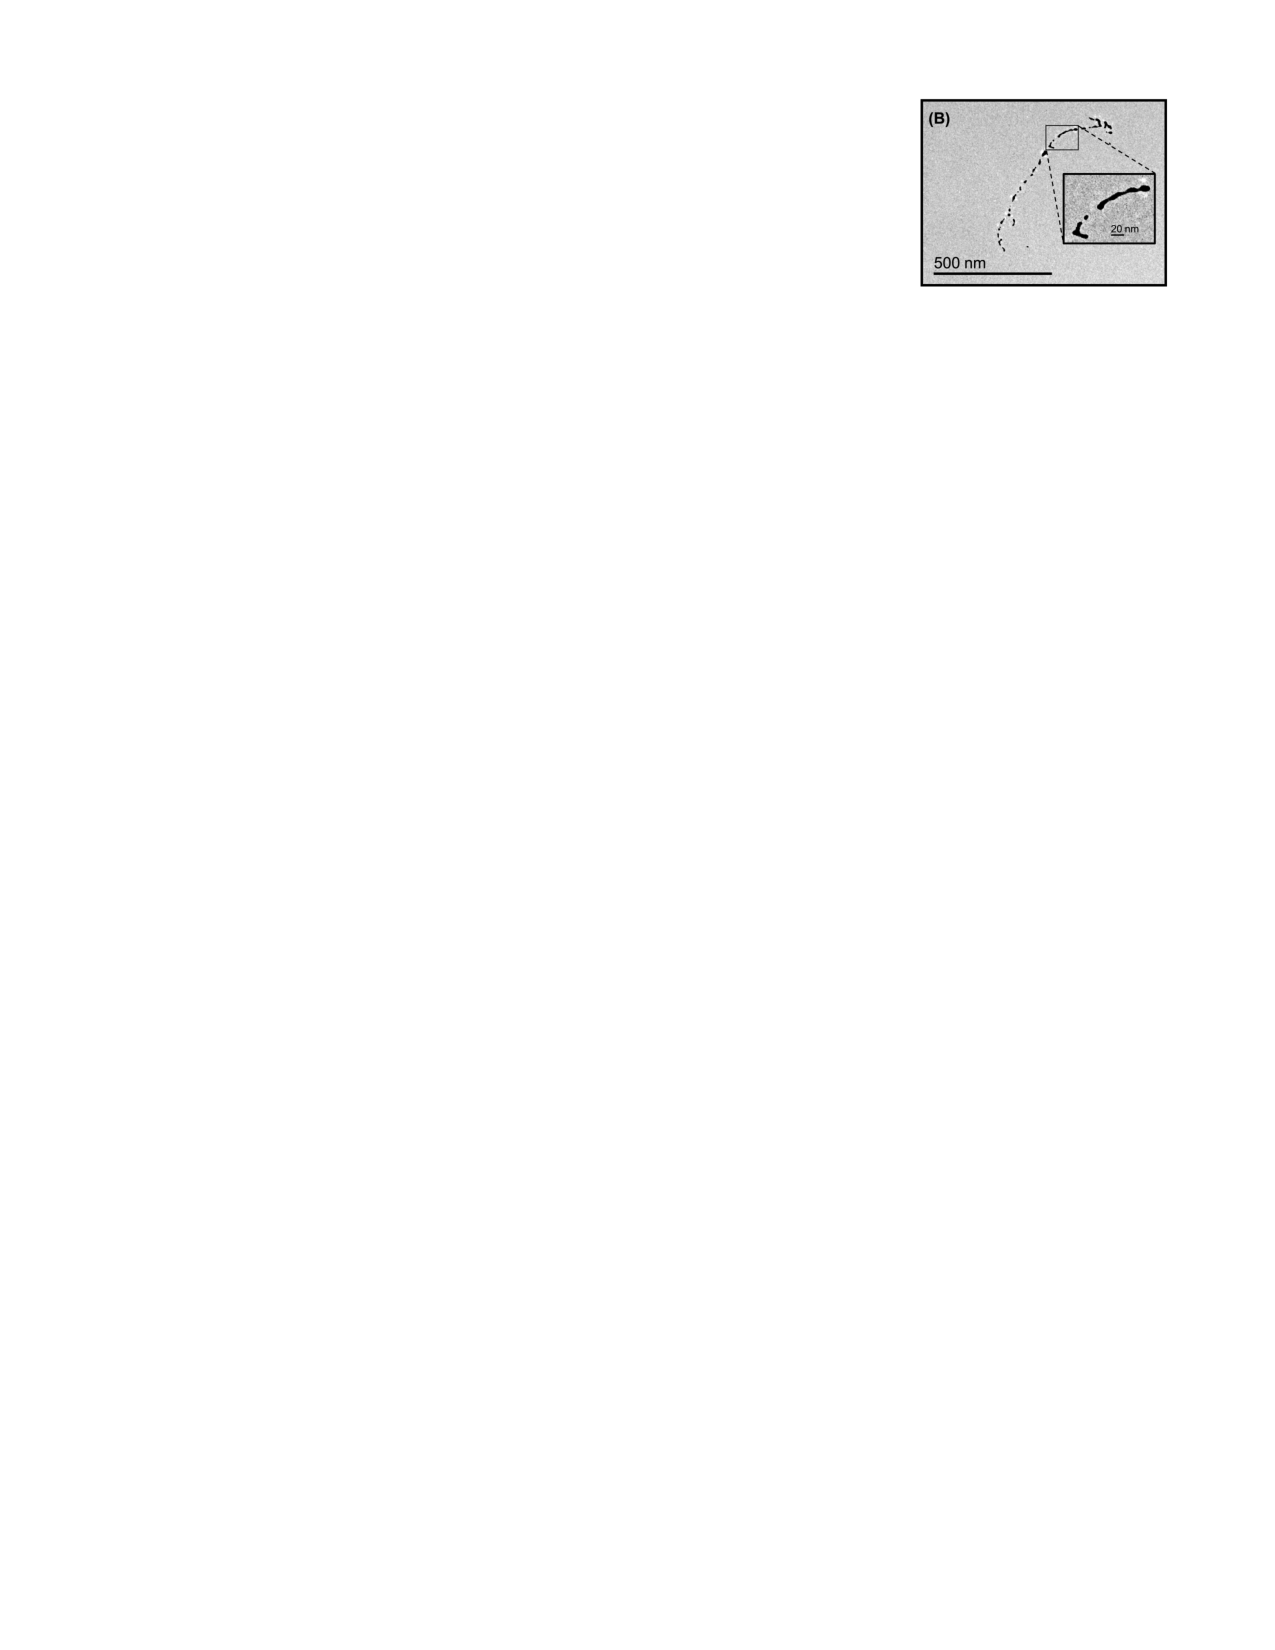
\includegraphics[width=0.75\textwidth]{silver-filament}
				\caption{Electron-microscope image of and elongated track-shaped Ag-cluster after it is surface-deposited.}
				\label{fig:silver-filament}
			\end{center}
		\end{figure}	
				
		\paragraph{Quantised vortices in He droplets} One of the most intriguing properties of superfluid helium droplets is the fact that they can host quantised vortices. Because of their ultra low temperature they are true quantum liquids and their vorticity and angular momentum are quantised. The existence of quantised vortices was anticipated because they have been created and observed in BECs made of dilute gases. However, the detection of quantised vortices is still experimentally challenging.
		
		\paragraph{The last few decades} A lot of of work has been done on helium droplets the last few decades, both experimentally and theoretically. From the absorption spectra of alkali metal doped helium droplets, the study of doped mixed $^3$He--$^4$He droplets, electrons in liquid helium, to the investigation of the critical Landau velocity inside small $^4$He droplet. For a comprehensive overview of work done in the last two decades, the interested reader is referred to the review papers[JLTP.Vol142.Nos.1/2(2006), IRPC.Vol36No4.621-707(2017), IRPC.Vol33No3.301-339(2014)].

%	\section{Structure of the thesis}
%		\lettrine[lines=3,findent=3pt,nindent=0pt]{T}{his} thesis will consist of two parts, since the presented work focusses on two distinct areas of interest with no mutual overlap. Each part will have its own short introduction to motivate the performed research and put in a broader context. The final chapter will conclude with some work in progress, planned work that has yet to start, and some ideas on how the method might be extended to be used in future research that is either cumbersome or impossible in its current form.
%
%		\subsection{Part I: Excited state dynamics}
%			In this part of the thesis the real-time dynamics of a single electronically excited rubidium (Rb) atom, residing in the surface dimple of a helium nano-droplet will be presented. The atom will be excited from its ground state 5s$^2\Sigma_{1/2}$ to the 5p$^2\{\Sigma,\Pi\}$ and 6p$^2\{\Sigma,\Pi\}$ manifold. This will be a combined experimental and theoretical study. The results are presented in two published articles:\\
%		
%			\emph{Imaging Excited-State Dynamics of Doped He Nanodroplets in Real-Time} will focus on imaging and characterising the dynamics using femtosecond spectroscopy and  time-dependent density functional theory.\\
%		
%			\emph{Desorption dynamics of RbHe-exciplexes off He nanodroplets induced by spin relaxation} is a combined experimental and theoretical investigation of the formation of free RbHe-exciplex molecules from laser-excited Rb-doped He nanodroplets through the mechanism of electronic spin relaxation. The role of relaxation of internal degrees of freedom of the RbHe exciplex in the desorption process has not been explicitly addressed.
%
%		\subsection{Part II: Collisions and capture by quantised vortices}
%			The second part investigates the real-time capture process of single xenon and argon atoms in their ground state by $^4$He$_{1000}$ droplets. Specifically it will address the interaction between a captured xenon or argon atom and a single quantised vortex line in the interior of the droplet. It will contain only theoretical investigations. The results will also be presented in two published works:\\
%		
%			\emph{Head-on Collisions of Xe Atoms Against Superfluid $^4\!$He Nanodroplets} studies the kinematics of head-on collisions between a xenon atom and a helium droplet. This scenario is then compared to a previous study of the same process with caesium to get a clear picture of the differences in dynamic behaviour between heliophilic and heliophobic species in said process. It also investigates different velocity regimes.\\
%		
%			\emph{Capture of Xe and Ar atoms by quantized vortices in $^4\!$He nanodroplets} addresses the capture of xenon and argon atoms at different velocity regimes and impact factors to determine the effective cross section for capture. This investigation then repeated with a dropet hosting one quantised line vortex. Also some preliminary results are presented for a larger droplet hosting an array of 6 line vortices, lined with argon atoms.
	\chapter{The DFT method for heavy impurities}\label{sec:dft-method}
	\epigraph{\flushright{One Functional to rule them all,\\
				One Functional to find them,\\
				One Functional to bring them all
				and in a droplet bind them.}}{\textit{F.M.G.J. Coppens}}

	\lettrine[lines=4,findent=3pt,nindent=0pt]{\color{activeColor}F}{rom} a theoretical point of view, superfluid helium must be considered as a high dimensional quantum system. Quantum Monte Carlo (QMC) \citep{Kro02} and direct quantum mechanical \citep{deL06,deL10,Agu13} calculations are the most accurate methods, but their computational demand quickly exceeds currently available computer resources when the number of helium atoms increases. Furthermore, QMC cannot describe dynamic evolution of superfluid helium in real time. To address these limitations, semi-empirical methods based on  density functional theory (DFT) formalism have been introduced\citep{Str87a,Str87b,Dal95}. DFT can be applied to much larger systems than QMC and allows for time-dependent formulation. As such, it offers a good compromise between accuracy and computational feasibility. The main drawback of DFT is that the exact energy functional is not known and must therefore be constructed in a semi-empirical manner. Moreover, doped helium droplets are limited to a mean-field description of the dopant-helium interaction. Nevertheless, DFT is the only method to date that can successfully reproduce results from a wide range of time-resolved experiments in superfluid helium, for realistic sizes compared to experimental conditions.
	
	\section{The Kohn-Sham approach}	\label{sec:kohn-sham}
		The starting point for the density functional method is the Hohenberg-Kohn (HK) theorem\citep{Hohenberg1964}, which states that the ground-state energy $E_v$ of an \emph{interacting inhomogeneous} system in a static potential $v$ can be written in as a unique functional of the one-body density $\rho$ as
		\begin{align}
			E_v[\rho] = \int\!v(\vec{r})\rho(\vec{r})\diff{r}+F[\rho] \label{eq1}
		\end{align}
		where $F[\rho]$ is a universal functional---valid for \emph{any} number of particles and \emph{any} external potential $v$---of the one-body density, defined as
		\begin{align}\label{eq:density-operator}
			\rho(\vec{r}) \vcentcolon= \ev**{\hat\rho(\vec{r})}{\Phi} = \ev**{\sum _{i=1}^{N}\delta(\vec{r}-\vec{r}_i)}{\Phi}
		\end{align}
		and $\Phi(\vec{r}_1,\vec{r}_2,\ldots,\vec{r}_N)$ is the many-body wave function of such a system. Furthermore, the functional $F[\rho]$ gives the ground state energy \emph{if and only if} the input density is the true ground state density of the system.
		
		Kohn and Sham (KS) later reformulated\citep{Kohn1965} the theory by introducing an approximation scheme for the functional $F[\rho]$ that is analogous to Hartree's method, but also contains the major part of the correlation effects inherent in interacting many-body systems. The approximation starts by defining
		\begin{align}
			F[\rho] \vcentcolon= T[\rho] + E_{c}[\rho]
		\end{align}
		where $T[\rho]$ is now the kinetic energy of a fictitious system of \emph{non-interacting} particles with density $\rho$ and $E_c[\rho]$ is the interaction term of an \emph{interacting} system with the same density, which contains all the other terms of the functional. For the kinetic part this allows us to write the total kinetic energy $T[\rho]$ as the sum of the individual kinetic energies $T_i$ of the non-interacting particles
		\begin{align}
			T = \sum_i T_i = -\frac{\hbar^2}{2m_4} \sum_i \ev**{\laplacian}{\varphi_i} = -\frac{\hbar^2}{2m} \sum_i \int\! \varphi_i^*({\mathbf r})\laplacian \varphi_i({\mathbf r})\diff{r}\,, \label{eq:kin-energy}
		\end{align}
		where $m_4$ is the mass of a $^4$He atom and the $\{\varphi_i\}$ are the Kohn-Sham single-particle orbitals corresponding to the many-body KS wave function $\Phi_{KS}(\vec{r}_1,\vec{r}_2,\ldots,\vec{r}_N)=\prod_i\varphi_i(\vec{r}_i)$ and leading to the density (using the definition in \eq{eq:density-operator}) $\rho(\vec{r})=\sum_i\absolutevalue{\varphi_i(\vec{r})}^2$.
	
		There is difference between the true kinetic energy of the interacting system and the fictitious one, due to the neglecting of the correlations. This difference is being corrected and accounted for in the correlation energy $E_c[\rho]$.
		
		Because the functional we used in this work is calibrated to produce the correct behaviour of bulk liquid helium at zero temperature $T=0$ and zero pressure $P=0$, we assume complete Bose-Einstein (BE) condensation of the helium. In this case all the helium atoms occupy the same single-particle KS-orbital $\varphi_0$. Therefore the many-body wave function and the density simplifies further to
		\begin{align}
			\Phi_{BEC}(\vec{r}_1,\vec{r}_2,\ldots,\vec{r}_N)=\prod_i\varphi_0(\vec{r}_i)
		\end{align}
		 and
		 \begin{align}
		 	\rho(\vec{r})=N\absolutevalue{\varphi_0(\vec{r})}^2
		 \end{align}
		 respectively. As explained in \scn{sec:bogol-order}, it is customary to define an effective wave function
		\begin{align}
			\Psi(\vec{r})\vcentcolon=\sqrt{\rho(\vec{r})}=\sqrt{N}\varphi_0(\vec{r}) \label{eq:order-param}	
		\end{align}
	 	for the condensate (see \eq{eq:order-param-real}), which is sometimes called a \emph{macroscopic wave function} or \emph{order parameter}. We can now simplify the expression for the kinetic energy (\eq{eq:kin-energy})
	%	\begin{align}
	%		T &= -\frac{\hbar^2}{2m} N \ev**{\laplacian}{\varphi_0} \nonumber \\
	%		  &= -\frac{\hbar^2}{2m} N\int\! \varphi_0^*(\vec{r})\laplacian \varphi_0(\vec{r})\diff{r} \nonumber \\
	%		 &= \frac{\hbar^2}{2m} N\int\! \abs{\grad{\varphi_0}}^2\diff{r} \label{eq5}
	%	\end{align}
		\begin{align}
			T = -\frac{\hbar^2}{2m_4} N\int\! \varphi_0^*(\vec{r})\laplacian \varphi_0(\vec{r})\diff{r}
			 = \frac{\hbar^2}{2m_4} N\int\! \abs{\grad{\varphi_0}}^2\diff{r}\,, \label{eq5}
		\end{align}	
		where we used partial integration to get to the last step and imposed that the orbital $\varphi_0$ vanishes at the boundaries. With our definition \eq{eq:order-param} we can now write the kinetic energy as a functional of the density
		\begin{align}
			T[\rho] = \frac{\hbar^2}{2m_4} \int\! \abs{\grad{\sqrt{\rho}}}^2\diff{r} 
		\end{align}
		To summarise, we write the complete energy functional $E_v$ as
		\begin{align}
			E_v[\rho] = \int\!v(\vec{r})\rho(\vec{r})\diff{r} + \frac{\hbar^2}{2m_4} \int\! \abs{\grad{\sqrt{\rho}}}^2\diff{r} + \int\!\mathcal{E}_c[\rho]\diff{r} \label{eq:ks-tot-energy}
		\end{align}
		where we defined the correlation energy density functional $\mathcal{E}_c$ through
		\begin{align}
			E_c[\rho] \vcentcolon= \int\!\mathcal{E}_c[\rho]\diff{r}\,.
		\end{align}
		The difficult job is to design a functional $\mathcal{E}_c$ such that the desired physical properties of helium can be recovered. This is far from trivial but several of these density functionals are available now. The one used in this work is discussed in \scn{sec:otdft}.
	
	\subsection{Time-dependent DFT}\label{sec:tddft}
	To describe the time evolution of the system, the Runge-Gross theorem extends DFT to its time-dependent version TDDFT\citep{Run84}. The functional variation of the associated action (see \eq{eq:action} for an example) leads to the following time-dependent Euler-Lagrange (EL) equation 
	\begin{align}
		i\hbar\frac{\partial}{\partial t} \Psi(\vec{r},t) = \left\{-\frac{\hbar^2}{2m_4}\laplacian + \fdv{\mathcal{E}_c}{\rho}\right\}\Psi(\vec{r},t) \vcentcolon= \mathcal{H}\qty[\rho]\Psi(\vec{r},t) 
		\label{eq:td-el-equation}
	\end{align}
	As long as we are in the thermodynamic regime the solutions $\Psi(\textbf{r},t)$ can be decomposed into the liquid density and associated velocity potential field (see \scn{sec:bogol-order} and \scn{sec:rot-vort}).
	
	Considering only eigenstates $\Psi(\vec{r},t)=\Psi_0(\vec{r})\unit{e}^{-i\mu t/\hbar}$ of the time independent Hamiltonian $\mathcal{H}\qty[\rho]$ the time-dependent EL-equation reduces to a time independent one
	\begin{align}
		\left\{-\frac{\hbar^2}{2m_4} \laplacian + \fdv{\mathcal{E}_c}{\rho}\right\}\Psi_0(\textbf{r}) = \mu\Psi_0(\textbf{r})
		\label{eq:el-equation}
	\end{align}
	with $\mu$ the chemical potential. Solving this equation by iteration will result in the ground state density $\abs{\Psi_0}^2$ of the system. Within the HK-framework and the variation principle that was used to obtain these EL-equations, the nature of the minimisation is such that it gives the lowest energy for a given symmetry. This means that as long as the input state does not break the symmetry of the time-independent EL-equation, it minimises the energy of this state even if it does not lead to the ground state. This can be used to obtain a stationary vortex-line solution. With the inclusion of appropriate constraints in the energy functional the same procedure can be used to obtain helium densities with an array of vortex-lines.

	\section{The Orsay-Trento Density Functional}\label{sec:otdft}
		\begin{table}
			\caption{Model parameters for the OT-DFT and solid functionals.}\label{tab:ot-params}
			\taburulecolor{activeColor}
			\begin{tabu} to \textwidth {X[c]X[c]X[c]X[2c]X[2c]X[c]}
				\toprule
				$\epsilon_{LJ}$~(K)	& $\sigma$~(\AA) & $h$~(\AA) & $c_2$~(K~\AA$^6$) & $c_3$~(K~\AA$^9$) & $\alpha_s$~(\AA$^3$) \\
				\midrule
				10.22 & 2.556 & 2.190323 & $-$2.41186~$\times~10^4$ & 1.85850~$\times~10^6$ & 54.31 \\
				&&&&& \\
				$\rho_{0s}$~(\AA$^{-3}$) & $l$~(\AA) & $C$~(Hartree) & $\beta$~(\AA$^3$) & $\rho_m$~(\AA$^{-3}$) & $\gamma_{11}$ \\
				\midrule
				0.04 & 1. & 0.1 & 40. & 0.37 & $-$19.7544 \\
				&&&&& \\
				$\gamma_{12}$~(\AA$^{-2}$) & $\alpha_1$~(\AA$^{-2}$) & $\gamma_{21}$ & $\gamma_{22}$~(\AA$^{-2}$) & $\alpha_2$~(\AA$^{-2}$) & \\ 
				\midrule
				12.5616 & 1.023 & $-$0.2395 & 0.0312 & 0.14912 & \\
				\bottomrule 
			\end{tabu}
		\end{table}

		\begin{figure}[t]
			\begin{center}
				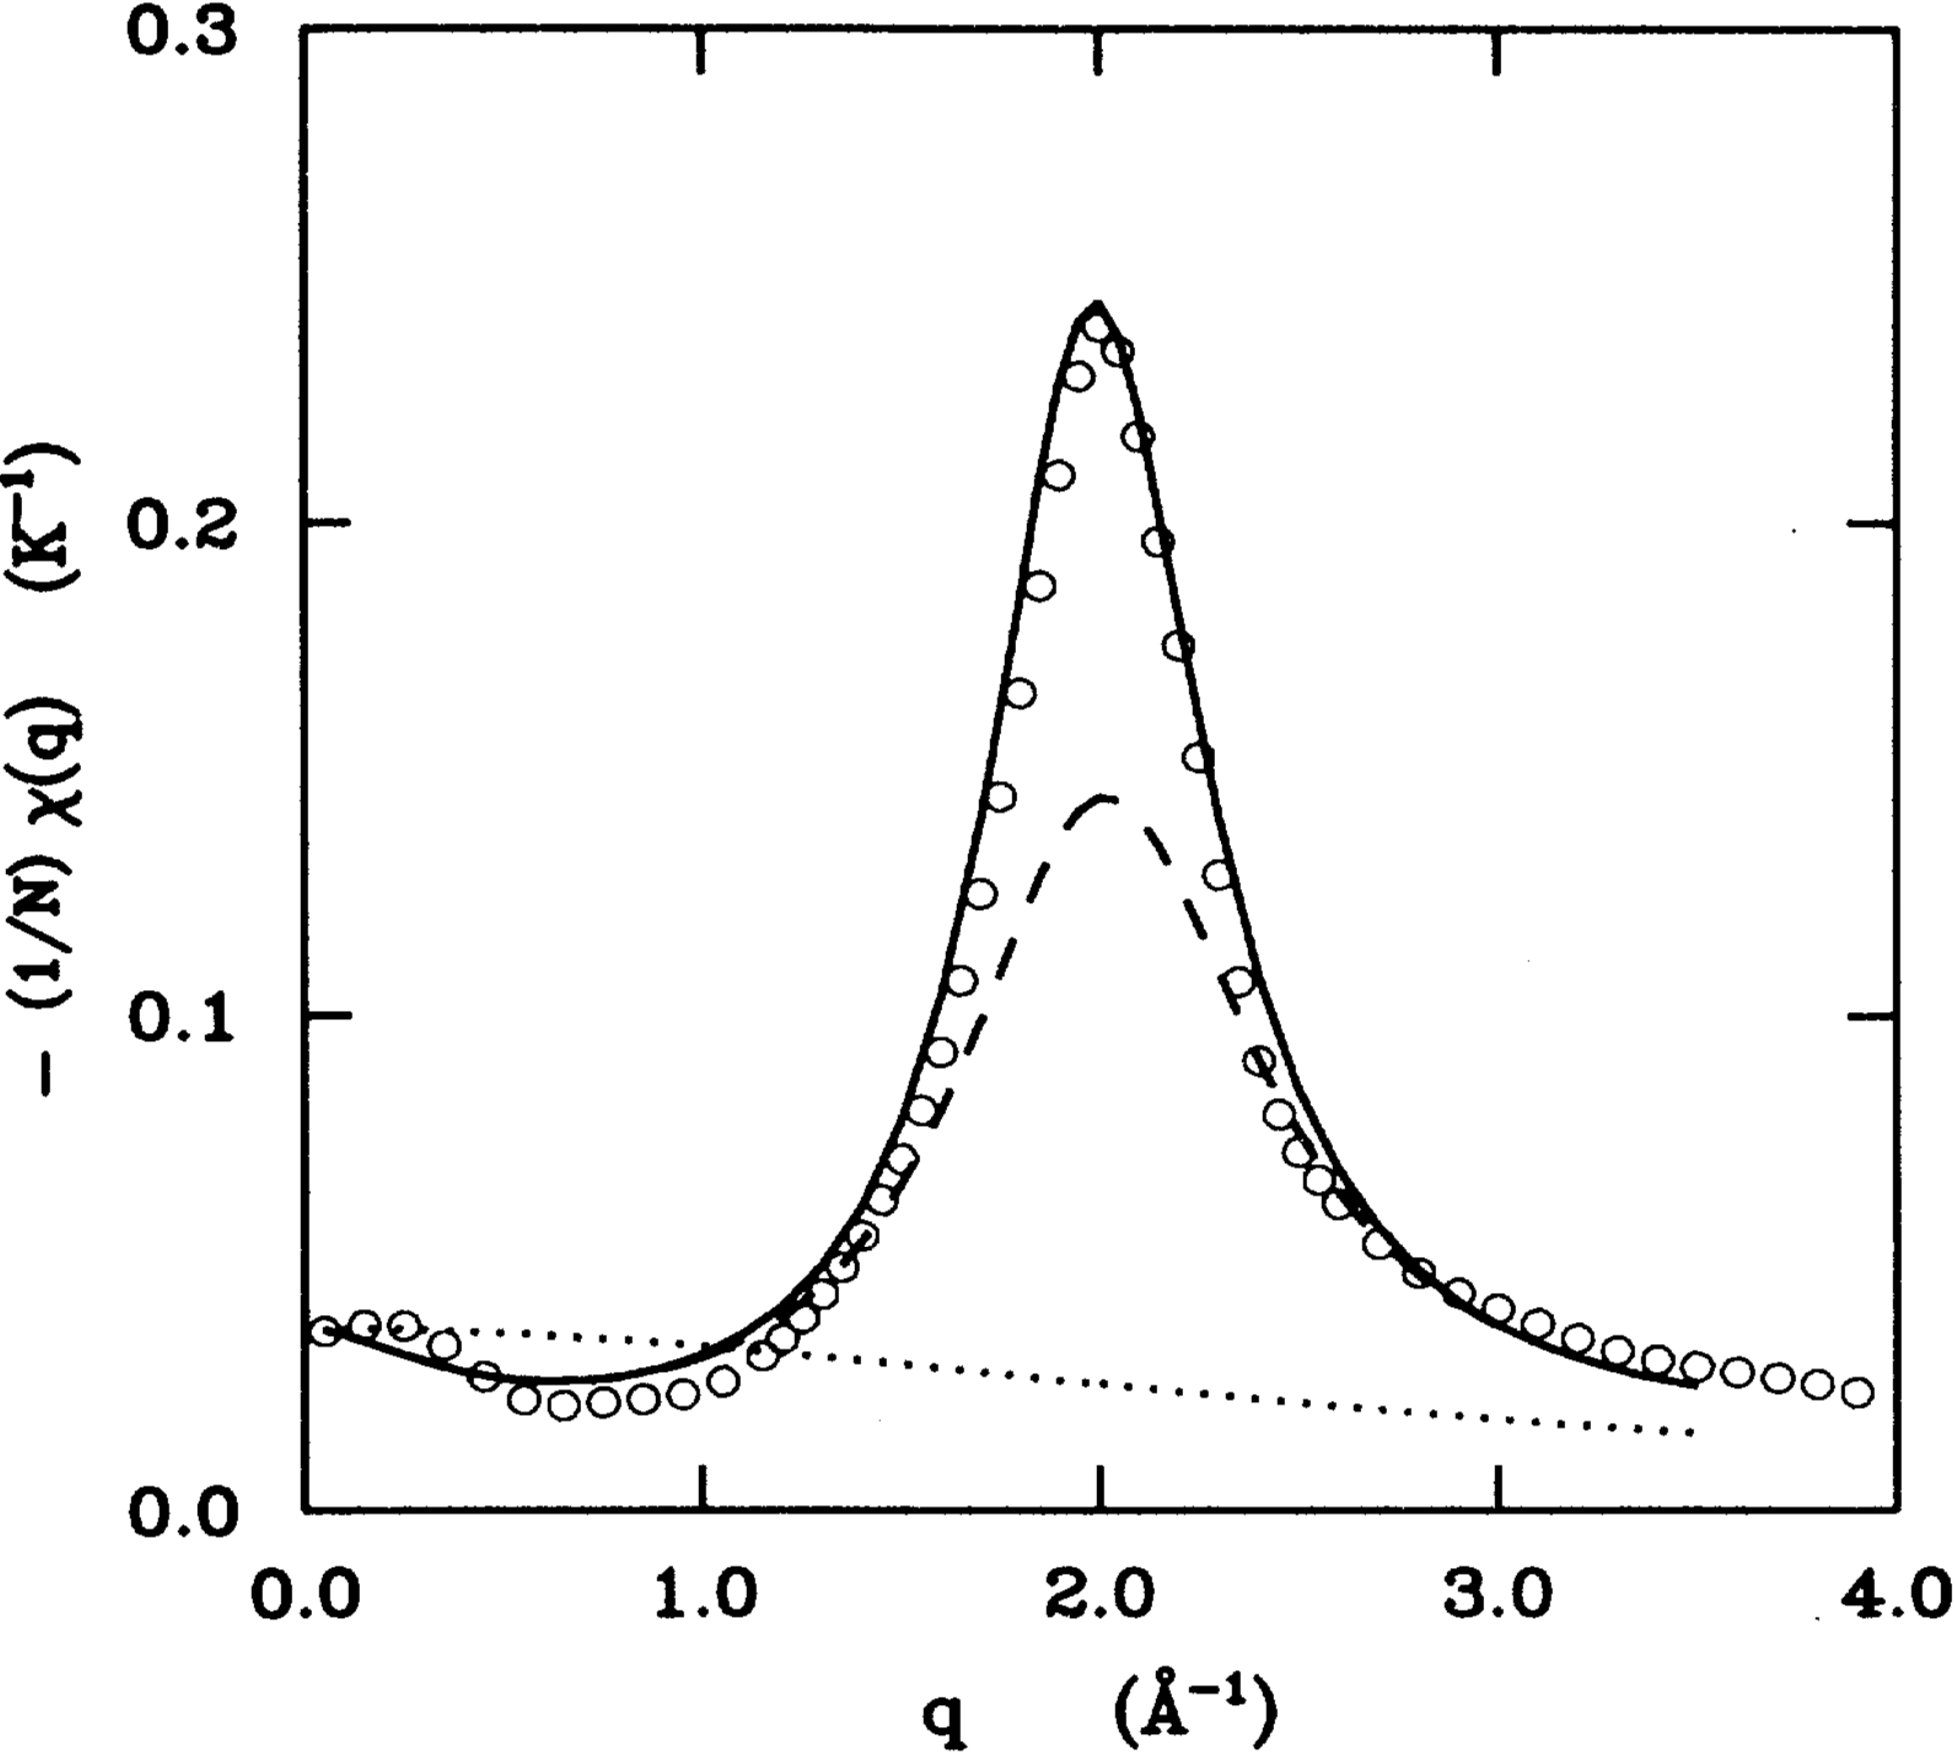
\includegraphics[width=0.75\textwidth]{static-response-function}
				\caption{Static response $-\chi$ (see\rf{Dalfovo1995}, Eqn.~(11)) per atom of liquid $^4$He at zero pressure. Points: experimental data; dotted line: from the functional of\rfs{Str87a,Str87b}; dashed line: Orsay-Paris (OP) functional\citep{Dupont-Roc1990}; solid line: OT functional.}
				\label{fig:static-response-function}
			\end{center}
		\end{figure}
	
		The functional that is used in the work presented in this thesis is based on the Orsay-Trento (OT) functional\citep{Dalfovo1995}. It uses a finite-range, non-local approach and it is, to date the most accurate model in the sense that its parameters were fitted to reproduce the bulk properties of liquid helium at $T=0=P$. It is written as
		\begin{align}
			\mathcal{E}_c[\rho ,\vec{v}] &=  
			\frac{1}{2} \left.\int \! \right\{\rho({\bf r}) V_{LJ}(|{\bf r}-{\bf r'}|) \rho({\bf r'}) \nonumber \\
			&+ \left.\frac{1}{2} c_2\, \rho({\bf r}) \left[{\bar \rho}({\bf r}) \right]^2 
			+ \frac{1}{3} c_3 \, \rho({\bf r}) \left[ {\bar \rho}({\bf r}) \right]^3\right\}\diff{r'} \nonumber \\
			&- \frac{\hbar^2}{4m_4} \alpha_s \int \! F(|{\bf r}-{\bf r'}|) \left[ 1- \frac{{\tilde \rho}({\bf r})}{\rho_{0s}} \right]\grad{\rho({\bf r})} \cdot \grad{\rho({\bf r'})} \left[ 1- \frac{{\tilde \rho}({\bf r'})}{\rho_{0s}} \right]\diff{r'} \nonumber \\
			& - \frac{m_4}{4} \int \! V_J(| \mathbf{r} - \mathbf{r}'|)\, \rho(\mathbf{r}) \, \rho(\mathbf{r}')\,  [\mathbf{v}(\mathbf{r})-\mathbf{v}(\mathbf{r}')]^2\diff{r'} \label{eq:otf}
		\end{align}
		The first term corresponds to a classical Lennard-Jones type two-body interaction between helium atoms. The interaction is screened at short distances where the interaction energy is of the same order as the correlation effects:
		\begin{align}
			V_{LJ}(r) = \begin{cases}
			\epsilon_{LJ} \left[\left(\frac{\sigma}{r} \right)^{12} - \left(\frac{\sigma}{r} \right)^{6} \right] & {\rm if} \quad r > h \\
			0 & {\rm otherwise}
			\end{cases}\label{eq9}
		\end{align}
		In the second line, the terms corresponding to $c_2$ and $c_3$, correct for short range correlations when $r<h$. The weighted density $\bar{\rho}$ is the average density $\rho$ over a sphere of radius $h$:
		\begin{align}
			\bar{\rho}(\vec{r}) = \int\!\Pi_h\qty(\abs{\vec{r}-\vec{r'}})\rho({\vec{r'}})\diff{r'},
		\end{align}
		with
		\begin{align}
			\Pi_h(r) \vcentcolon= \begin{cases}
				\frac{3}{4\pi h^3} & \rm{if} \quad r\leq h \\
				0 & \rm{otherwise}
			\end{cases}
		\end{align}
		The third line is a non-local correction to the kinetic energy (KC). It partially accounts for the difference $\mathcal{T}[\rho]-T[\rho]$ mentioned in \scn{sec:kohn-sham}. The gradient-gradient interaction function $F$ is a Gaussian kernel defined as
		\begin{align}
			F(r) = \frac{1}{l^3\sqrt{\pi^3}}\unit{e}^{-r^2/l^2}
		\end{align}
		All the parameters are fitted to reproduce the peak of the static response function (see \fig{fig:static-response-function}) in the bulk liquid. The factor $\qty(1-\tilde{\rho}/\rho_{0s})$ is included to match the pressure dependence of the static response function predicted by diffusion Monte Carlo calculations\citep{Moroni1992}. The quantity $\tilde{\rho}(\vec{r})$ is another weighted density, calculated using $F$ as a weight
		\begin{align}
			\tilde{\rho}(\vec{r}) \vcentcolon= \int\!F\qty(\abs{\vec{r}-\vec{r'}})\rho(\vec{r'})\diff{r'}
		\end{align}
		The density $\tilde{\rho}(\vec{r})$ is very close to the normal density $\rho(\vec{r})$ except in very inhomogeneous situations. For pure helium droplets and free helium surfaces one can safely use $\rho$ instead of $\tilde{\rho}$. In the presence of significant short-range density oscillations, e.g. in the presence of heavy atomic impurities as presented in this thesis or electrons, the helium density needs to be smoothed by the Gaussian kernel $F$.  
			
		Finally, the last line in \eq{eq:otf} is called the \emph{back-flow} term and influences the dynamic response of the system. It plays the role of a non-local kinetic energy. Since the back-flow contains the factor $\vec{v}-\vec{v'}$, with $\vec{v}$ defined in \eq{eq:velocity-field}, the contribution will only be non-zero whenever the effective wave function $\Psi$ is complex-valued. Consequently, for time-independent cases it means that this will only affect the vortex states. The phenomenological effective current-current interaction $V_J(r)$ is calibrated so that it reproduces the experimental phonon-roton spectrum (see \fig{fig:dispersion-relation}):
		\begin{align}
			V_J(r) =\,&(\gamma_{11} +\gamma_{12} \, r^2) e^{-\alpha_1 r^2} \nonumber \\
				+\,&(\gamma_{21} +\gamma_{22} \, r^2) e^{-\alpha_2 r^2}
		\end{align}
		All the parameters of the functional are given in \tab{tab:ot-params}.

		\subsection{The Solid-OT Density Functional}
			In the presence of highly inhomogeneous liquid densities, e.g. atomic impurities with a very strong He-X interaction, the OT-functional \eq{eq:otf} becomes numerically unstable. To deal with this problem an additional cut-off can be used
			\begin{align}
				\mathcal{E}^\mathrm{sol} \vcentcolon= C\rho(\vec{r})\qty{1+\tanh(\beta\qty[\rho(\vec{r})-\rho_\mathrm{m}])}
			\end{align}
			where the model parameters $\qty{C,\beta,\rho_\mathrm{m}}$ are specified in \tab{tab:ot-params}. Including this term in the OT-functional prevents excessive density build-up. $\mathcal{E}^\mathrm{sol}$ only starts to deviate from zero whenever the liquid density $\rho$ is comparable to $\rho_\mathrm{m}$ or larger. Therefore, inclusion of this term in the functional does not alter the density distribution. This penalty term was originally developed to account for the liquid-solid phase transition of $^4$He\citep{Anc05a,Cau07}. The functional that has been used to obtain the result presented in this work is refered to as the ``Solid-OT-DFT functional''. It consists of the first three terms of the original OT-functional \eq{eq:otf}, plus $\mathcal{E}^\mathrm{sol}$
			\begin{align}
				\mathcal{E}_c^\mathrm{sol}[\rho] &=  
				\frac{1}{2} \left.\int \! \right\{\rho(\vec{r}) V_{LJ}(\abs{\vec{r}-\vec{r'}}) \rho(\vec{r'}) \nonumber \\
				&+ \left.\frac{1}{2} c_2\, \rho(\vec{r}) \qty[\bar\rho(\vec{r})]^2 
				+ \frac{1}{3} c_3 \, \rho(\vec{r}) \qty[\bar\rho(\vec{r})]^3\right\}\diff{r'} \nonumber \\
				&+ C\,\rho(\vec{r})\qty\Big{1+\tanh(\beta\qty[\rho(\vec{r})-\rho_\mathrm{m}])} \label{eq:solid-otf}
			\end{align}

	\section{Static calculations}
		In the work presented here all the impurities are heavy compared to the mass of $^4$He, e.g. the mass of rubidium (Rb) is about 21 times larger than that of helium (He), xenon (Xe) roughly 33 times and argon (Ar) about 10 times. Therefore we are allowed to treat the centre of mass motion of the impurities as classical. It was also checked for potassium (K) which is slightly lighter than Ar\citep{Martinez2017}. In the functional this will be modelled as an external field $V_X$, the impurity-He pair interaction
		\begin{align}
			E[\rho] \rightarrow E[\rho] + \!\int\!\rho(\vec{r})\,V_X\qty(\abs{\vec{r}-\vec{r}_I})\diff{r} \label{eq:el-static-hi}
		\end{align}
		where ${\vec r}_I$ is the location of the impurity. Varying the modified functional to minimise the energy one now finds a new EL-equation in which the helium--impurity interaction is included:
		\begin{align}
			\left\{-\frac{\hbar^2}{2m_4} \laplacian + \fdv{\mathcal{E}_c}{\rho} + V_X(|{\mathbf r} - {\mathbf r_I}|)\right\}\Psi({\mathbf r}) = \mu \Psi({\mathbf r}) \label{eq:el-static-hi}
		\end{align}
		This equation is then solved by iteration in a self-consistent way by the imaginary time propagation method\citep{Lehtovaara2007} (ITM) in cartesian coordinates. The calculations are performed in three dimensions without imposing any symmetries that are present in the external potential. All the quantities are discretised on an evenly spaced Cartesian grid with a step-size that is typically of the order of 0.4~\AA. The differential operators are evaluated using a $k$-point finite difference method where in most applications $k=13$ is sufficiently accurate. The integrals in the density-functional can be expressed as convolutions and can therefore be evaluated in momentum-space by exploiting the convolution theorem, using proprietary highly optimised parallel Fast Fourier Transform algorithms. 
			
		\subsection{Producing vortical states}\label{sec:vortical-states}
			The helium density that minimises the energy of the vortical states $\Psi_s$ (\eq{eq:line-vortex}), introduced in \scn{sec:rot-vort}, can be obtained by solving the same EL-equation as for a vortex-free droplet. This becomes clearer when we write \eq{eq:el-equation} in cylindrical coordinates:
			\begin{align}
				\qty{-\frac{\hbar^2}{2m_4}\qty[\frac{1}{r}\pdv{r}\qty(r\pdv{r})-\frac{s^2}{r^2}]+\fdv{\mathcal{E}_c}{\rho}}\Psi_s(\vec{r}) = \mu\Psi_s(\vec{r}) \label{eq:el-cyl}
			\end{align}
			Written like this it is evident that the ground state $\Psi_0$ is just the special case for $s=0$. Obtaining the solution using the ITM works as long as the solution has overlap with initial guess for the order parameter. Starting with a trial order parameter similar to $\Psi_s$ will guarantee this. To do this we apply the ``imprinting'' technique where we apply the ground state density of a previously obtained vortex-free droplet and multiply it with a normalised complex factor
			\begin{align}
				\Psi(\mathbf{r}) = \sqrt{\rho_0(\vec{r})} \,\times \frac{x + iy}{\sqrt{x^2 + y^2}} \label{eq28}
			\end{align}
			where $\rho_0$ is the ground state density of the vortex-droplet.  In cylindrical coordinates this factor is equivalent to the one in \eq{eq:line-vortex} for $s=1$. 
			
			This changes for droplets with two or more vortices, where the cylindrical symmetry is broken and the solutions are no longer solutions of \eq{eq:el-cyl}, nor eigenfunctions of the angular momentum operator. In this case the time-independent EL-equation has to be modified to include a rotational constraint solution in the co-rotating frame
			\begin{align}
				{\cal H} \rightarrow {\cal H}-\Omega \hat{L}_z
			\end{align}
			 such that for a suitable choice of $\Omega$ the vortex-array solution becomes favourable to the ground state and also to excited states with angular momentum $s\geq 2$. Since these states are no longer eigenstates of the original time-dependent Hamiltonian, these states are no longer stationary and will start to rotate with frequency $\Omega$. The initial guess for a droplet with $n_v$ vortices can be produced using the same imprinting method as mentioned before		
			\begin{align}
				\Psi(\mathbf{r})=\sqrt{\rho_0(\vec{r})} \times \prod _{j=1}^{n_v}\left[ {(x-x_j)+i(y-y_j) \over \sqrt{(x-x_j)^2+(y-y_j)^2}}  \right] \label{eq32}
			\end{align}
			where $\rho_0$ is again the ground state density of the vortex-free droplet and $(x_j,y_j)$ is the initial position of the $j$-th vortex-line parallel to the $z$-axis.

	\section{Dynamic calculations}\label{sec:td-dft}
		For the dynamic evolution of atomic impurities excited from $n$s-states to $n'$s-states, we do not need to keep track of the evolution of the electronic state of the impurity since it keeps its spherically symmetric orbital. In this case we only need to describe the time evolution of the centre of mass coordinate of the impurity. As in the statics, because of the large atomic mass of the impurity compared to helium, the time evolution of the centre of mass coordinate of the impurity is treated classically. To obtain the correct energy for the whole droplet-impurity system the energy functional needs to be extended to include the impurities centre of mass motion and the impurity-helium interaction
		\begin{align}
			E[\rho] \rightarrow E[\rho] + \frac{p^2_I}{2 m_I} + \int \! \rho(\mathbf{r}) \, V_{X^{\!*}}\qty(\abs{\vec{r}-\vec{r}_I})\diff{r} \label{eq33}
		\end{align}
		where $p_I$ is the classical momentum of the impurity (which was not present in the static case, \eq{eq:el-static-hi}), $m_I$ is the impurity mass and $V_{X^{\!*}}$ is the impurity-He pair interaction potential for an impurity in the ground-, excited $n'$s- or ionised state. The equations of motion for the time evolution of the effective wave function $\Psi\qty(\vec{r},t)$ and the second time derivative of the impurity location $\ddot{\vec{r}}_I$ are  
		\begin{align}
			i\hbar\frac{\partial}{\partial t} \Psi &= \qty[-\frac{\hbar^2}{2m_4} \laplacian +\frac{\delta {\cal E}_c}{\delta \rho} + V_{X^*}(|\mathbf{r}- \mathbf{r}_I|)]\Psi\nonumber\\
			m_I \ddot{\mathbf{r}}_I &= - \grad_{\vec{r}_I} \left[  \int \!\rho(\mathbf{r}) V_{X^*}(|\mathbf{r}- \mathbf{r}_I|)\diff{r}  \right] \nonumber \\
			&= -\int \! V_{X^*}(|\mathbf{r}- \mathbf{r}_I|)  \, \grad \rho(\mathbf{r})\diff{r} \label{eq34}
		\end{align}
	
		\subsection{Diatomics in Molecules}\label{sec:dim-model}
			\begin{figure}[t]
				\begin{center}
					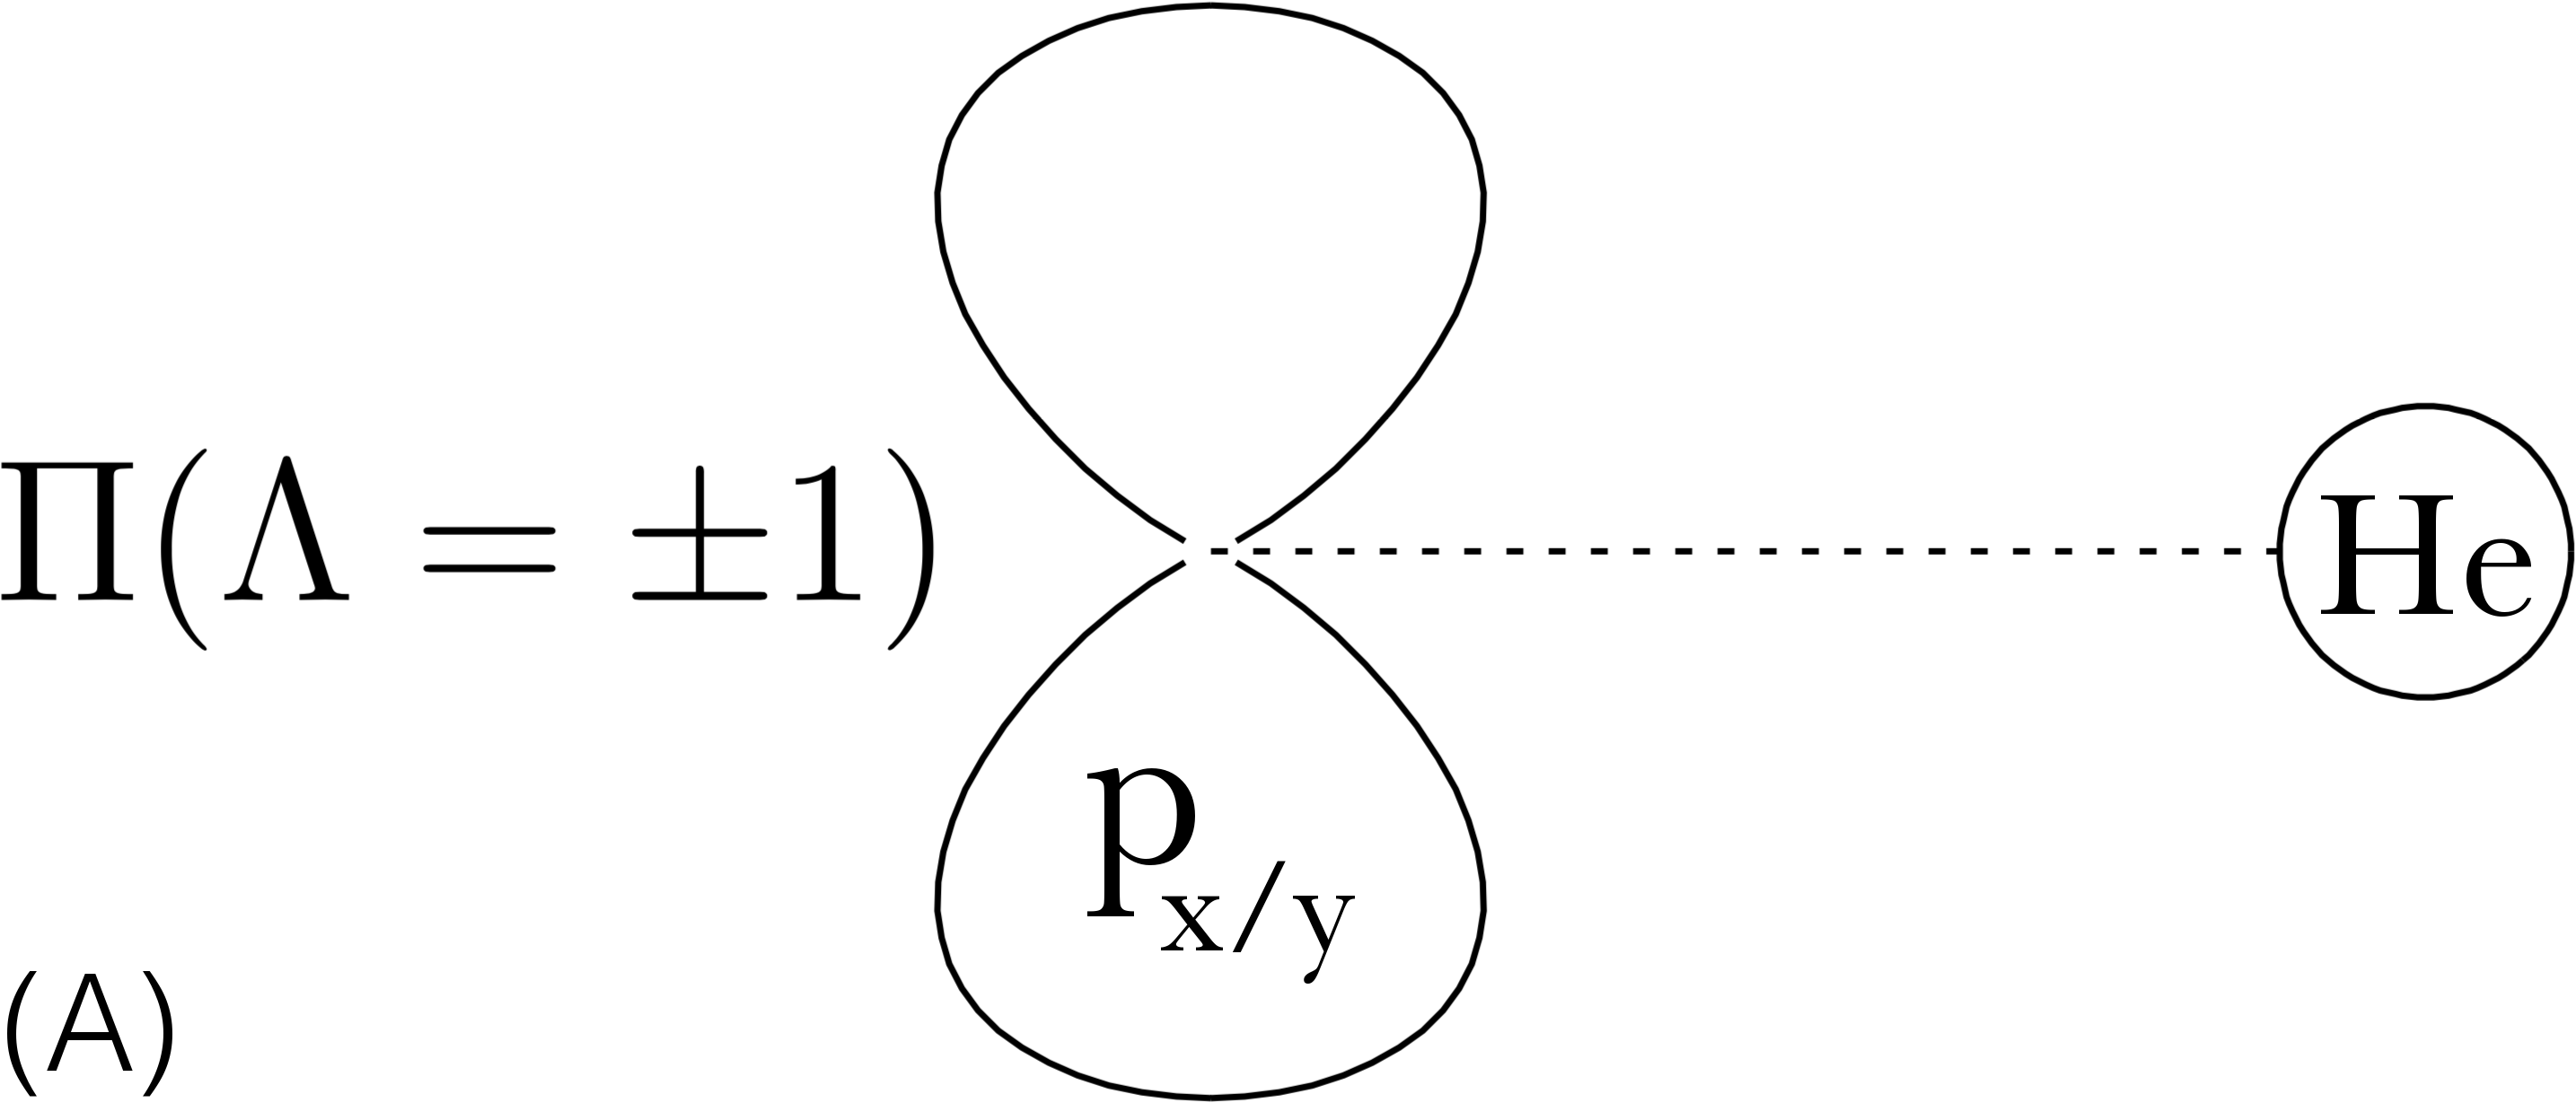
\includegraphics[width=0.45\textwidth]{pxy-he}
					\hspace{20pt}
					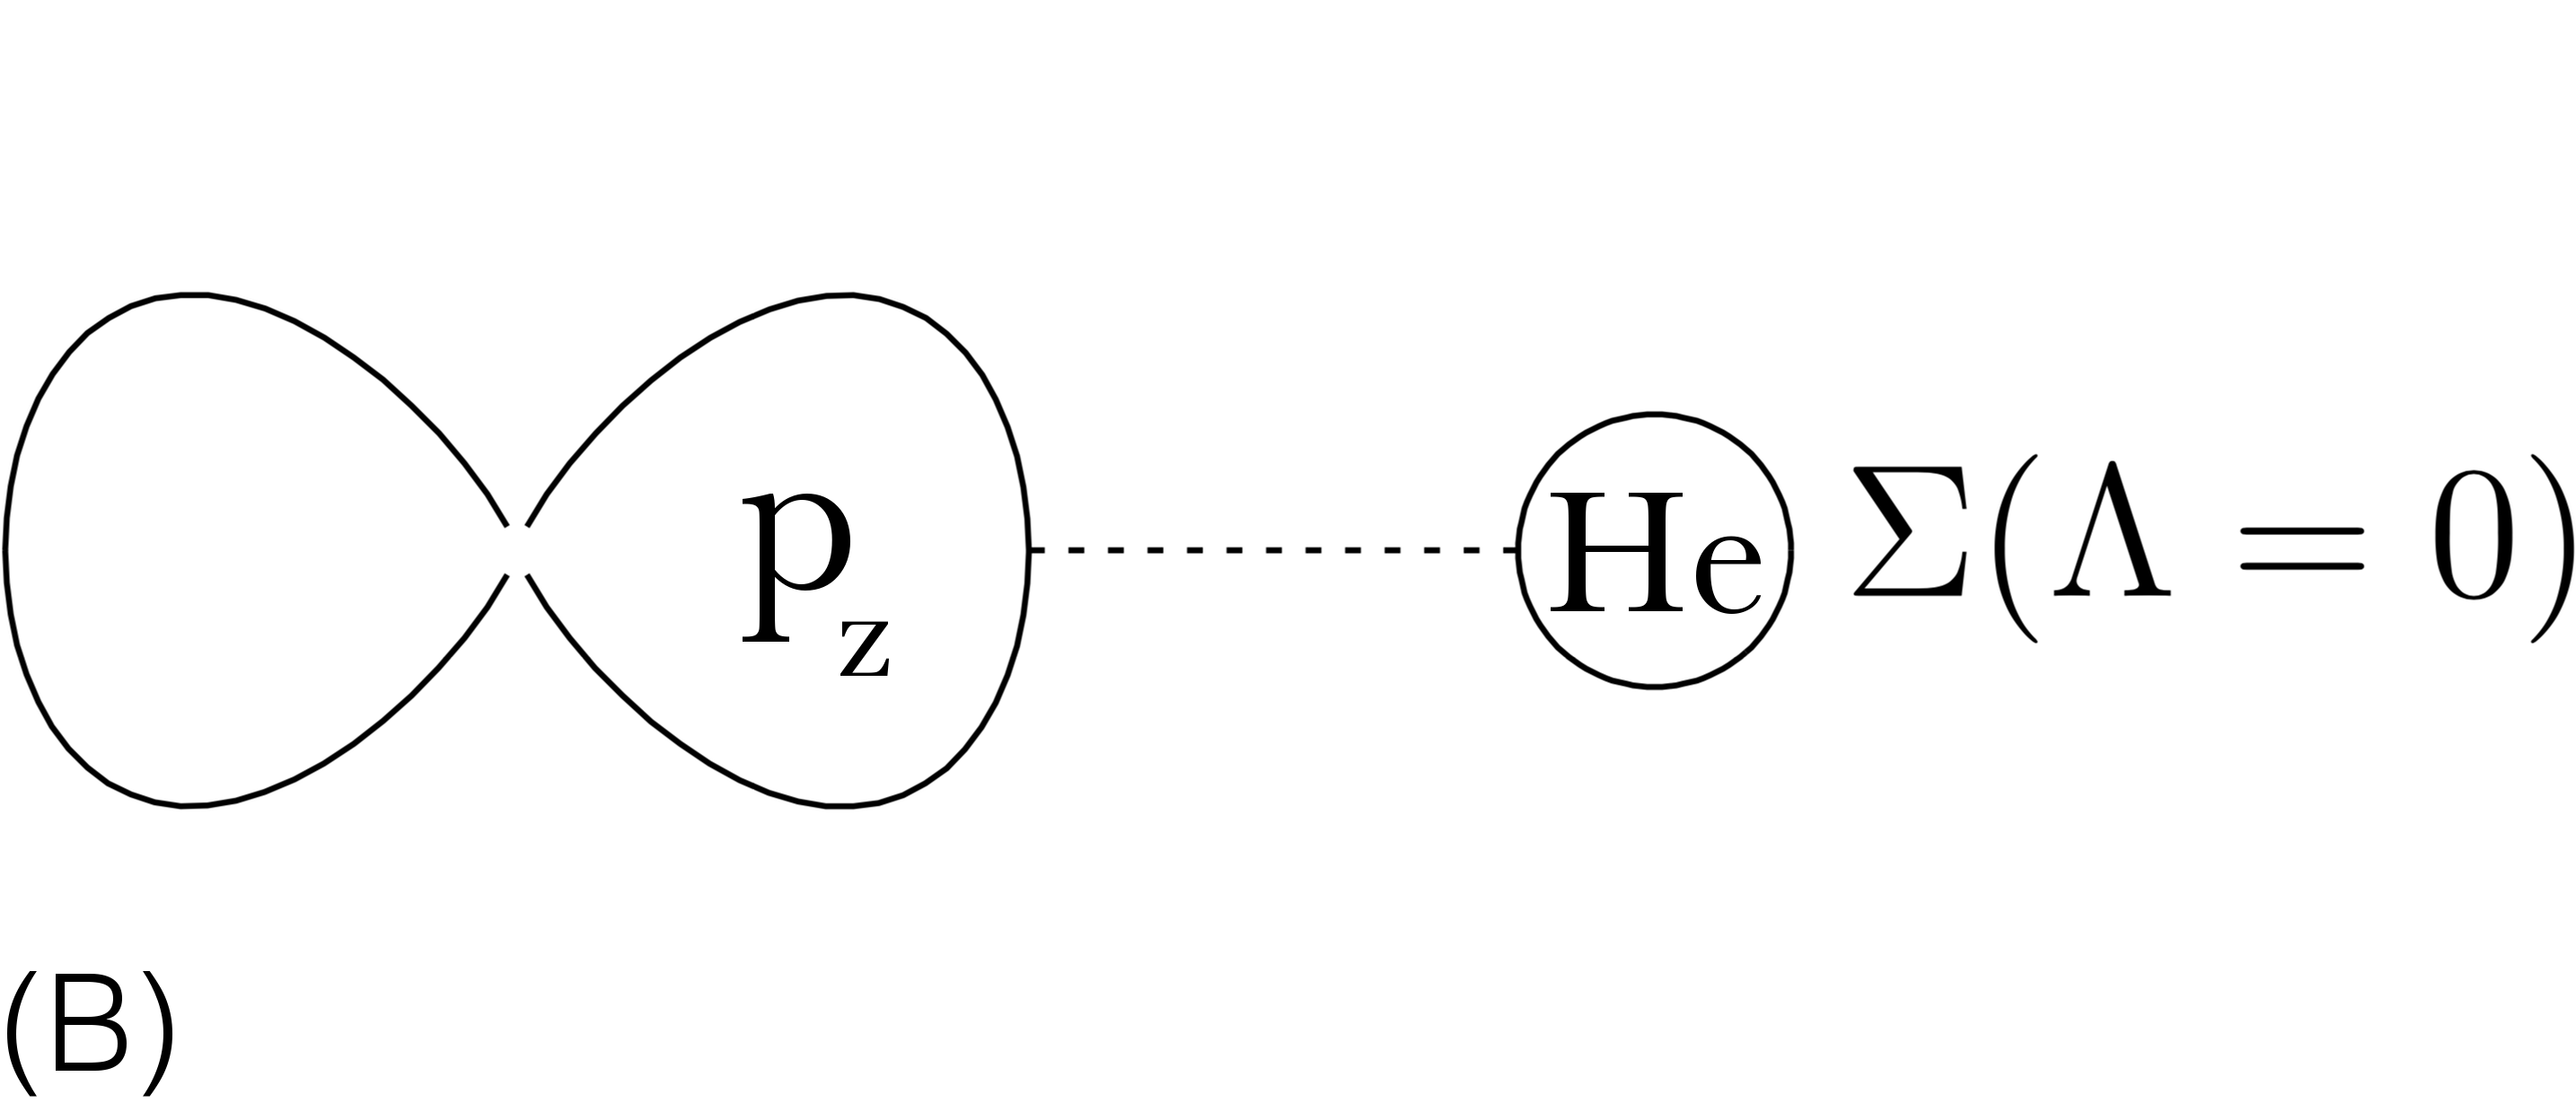
\includegraphics[width=0.45\textwidth]{pz-he}
				\end{center}
				\caption{Level splitting of the p-orbitals in the presence of helium, that breaks the spherical symmetry. (A)~A double degenerate n'p$_\mathrm{x/y}$-orbital and (B)~a single n'p$_\mathrm{z}$-orbital. (Illustration courtesy of M. Martinez\citep{Martinez2017}.)}
				\label{fig:p-orbitals}
			\end{figure}				
			The situation becomes slightly more complicated for $n$s-states excited to $n'$p-states (effective one-electron excited $^2$P-states). Since the three p-orbitals are no longer spherically symmetric and start mixing due to the interaction with the He droplet and spin-orbit coupling, we also need to include a description that accounts for the mixing of these orbitals in a dynamic way. To do this we use Diatomics in Molecules\citep{Ellison1963}(DIM). The interaction between a helium atom ($^1$S$_0$-state) and the triply degenerate $L=1$ electronic state of the impurity partially lifts the degeneracy so that the interaction can be decomposed into a $\Sigma$-state and a doubly degenerate $\Pi$-state (see \fig{fig:p-orbitals}). In the cylindrical symmetry it is customary to use the molecular term symbol $^{2S+1}\Lambda_\Omega$ to label the levels. In the bound region of the potentials $S$ is the electronic spin angular momentum (and $2S+1$ the spin multiplicity), $\Lambda$ is the quantum number for the projection of the electronic orbital angular momentum and $\Omega$ is the total electronic angular momentum, along the internuclear axis. Or symbolically
			\begin{align}
				m_j=m_l+m_s\:\longrightarrow\:\Omega=\Lambda+m_s
			\end{align}
			 Following the spectroscopic notation the orbitals corresponding to $\Lambda=0,1,2,3,\ldots$ are labeled $\Sigma,\Pi,\Delta,\Phi,\ldots$. The state vector of the impurity interacting with a He atom can be expressed in an uncoupled basis
			\begin{align}
				 \ket{p_{im}}\in\qty\big{\,\ket{p_{xm}}\!,\ket{p_{ym}}\!,\ket{p_{zm}}} \label{eq:dim-basis}
			\end{align}
			of real one-electron p-orbitals oriented along the internuclear axis (see \fig{fig:dim-axes}). The helium-impurity interaction matrix is given by
			\begin{align}
				\mathcal{V}^{DIM}(r_m) &= V_{\Pi}(r_m)\qty\big(\dyad{p_{xm}}+\dyad{p_{ym}})+V_{\Sigma}(r_m)\dyad{p_{zm}} \nonumber \\
					&= V_{\Pi}(r_m)\qty\big(\mathbb{1}_3-\dyad{p_{zm}})+V_{\Sigma}(r_m)\dyad{p_{zm}} \nonumber \\
					&=V_{\Pi}(r_m)\mathbb{1}_3+\qty\big[V_{\Sigma}(r_m)-V_{\Pi}(r_m)]\dyad{p_{zm}}
			\end{align}	
			where $r_m$ is the modulus of the interatomic separation vector and $V_\Pi$ and $V_\Sigma$ are the $\Pi$ and $\Sigma$ impurity-He pair potentials in the absence of spin-orbit coupling. For a system consisting of $N$ helium atoms the total interaction energy is calculated by summing over all the contributions of the $N$ individual $^4$He--X contributions
			\begin{align}
				\mathcal{U}^{DIM}(\vec{r}_I)=\sum_{m=1}^{N}\mathcal{V}^{DIM}(r_m)
			\end{align}
			It is more convenient to express the interaction in a basis common to all impurity-helium pairs, instead of a basis that depends on the particular impurity-helium pair chosen. To do this we apply a rotation $\mathcal{R}_m:\hat{\vec{z}}_m\mapsto\hat{\vec{z}}\propto\vec{r}_I$, so that the matrix corresponding to the $m^{\rm th}$ $^4$He atom expressed in the common basis is given by
			\begin{align}
				\dyad{p_{zm}} = \mathcal{R}_m\dyad{p_z}\mathcal{R}_m^{-1}
			\end{align}
			It can be shown that the elements of this matrix in cartesian coordinates are of the form
			\begin{equation}
				\mel**{p_i}{\mathcal{R}_m\dyad{p_z}\mathcal{R}_m^{-1}}{p_j} = \frac{r_{im}\,r_{jm}}{\norm{\vec{r}_m}^2}		\label{eq39}
			\end{equation}	
			where $(i,j)\in\qty{x,y,z}$. With these definitions we can write the matrix elements $U^{DIM}_{ij}$ of the interaction energy $\mathcal{U}^{DIM}$
			\begin{align}
				U^{DIM}_{ij}(\vec{r}_I)=\mel**{p_i}{\mathcal{U}^{DIM}}{p_j} = \sum_{m=1}^{N} V^{DIM}_{ij}(r_m)
			\end{align}
			where
			\begin{align}
				V^{DIM}_{ij}(r_m) \vcentcolon= V_\Pi(r_m)\delta_{ij}+\qty\Big[V_\Sigma(r_m)-V_\Pi(r_m)]\frac{r_{im}\,r_{jm}}{\norm{\vec{r}_m}^2} \label{eq:vdim}
			\end{align}
			are the matrix elements of $\mathcal{V}^{DIM}$ expressed in the common basis. Since we are working with a continuous helium density $\rho(\vec{r})$ and not with discrete atoms, the summation over $N$ helium atoms in the previous expression is replaced by an integral over the density $\sum_m\rightarrow\int\!\rho(\vec{r})\diff{r}$. Here we dropped the subscript $m$, representing the $m^\mathrm{th}$ helium atom. This finally gives for the matrix element $U^{DIM}_{ij}$
			\begin{align}
				U^{DIM}_{ij}(\vec{r}_I) = \int\! \rho\qty(\vec{r}+\vec{r}_I)\,V^{DIM}_{ij}(r)\diff{r} \label{eq:u-dim}
			\end{align}
			
			The eigenvalues $U^{\mathrm{np}}_k(\vec{r}_I)$ of this real symmetric matrix define the potential energy curves (PECs) without spin-orbit coupling as a function of the distance between the surrounding helium and the impurity for a given helium density.
			\begin{figure}[t]
				\begin{center}
					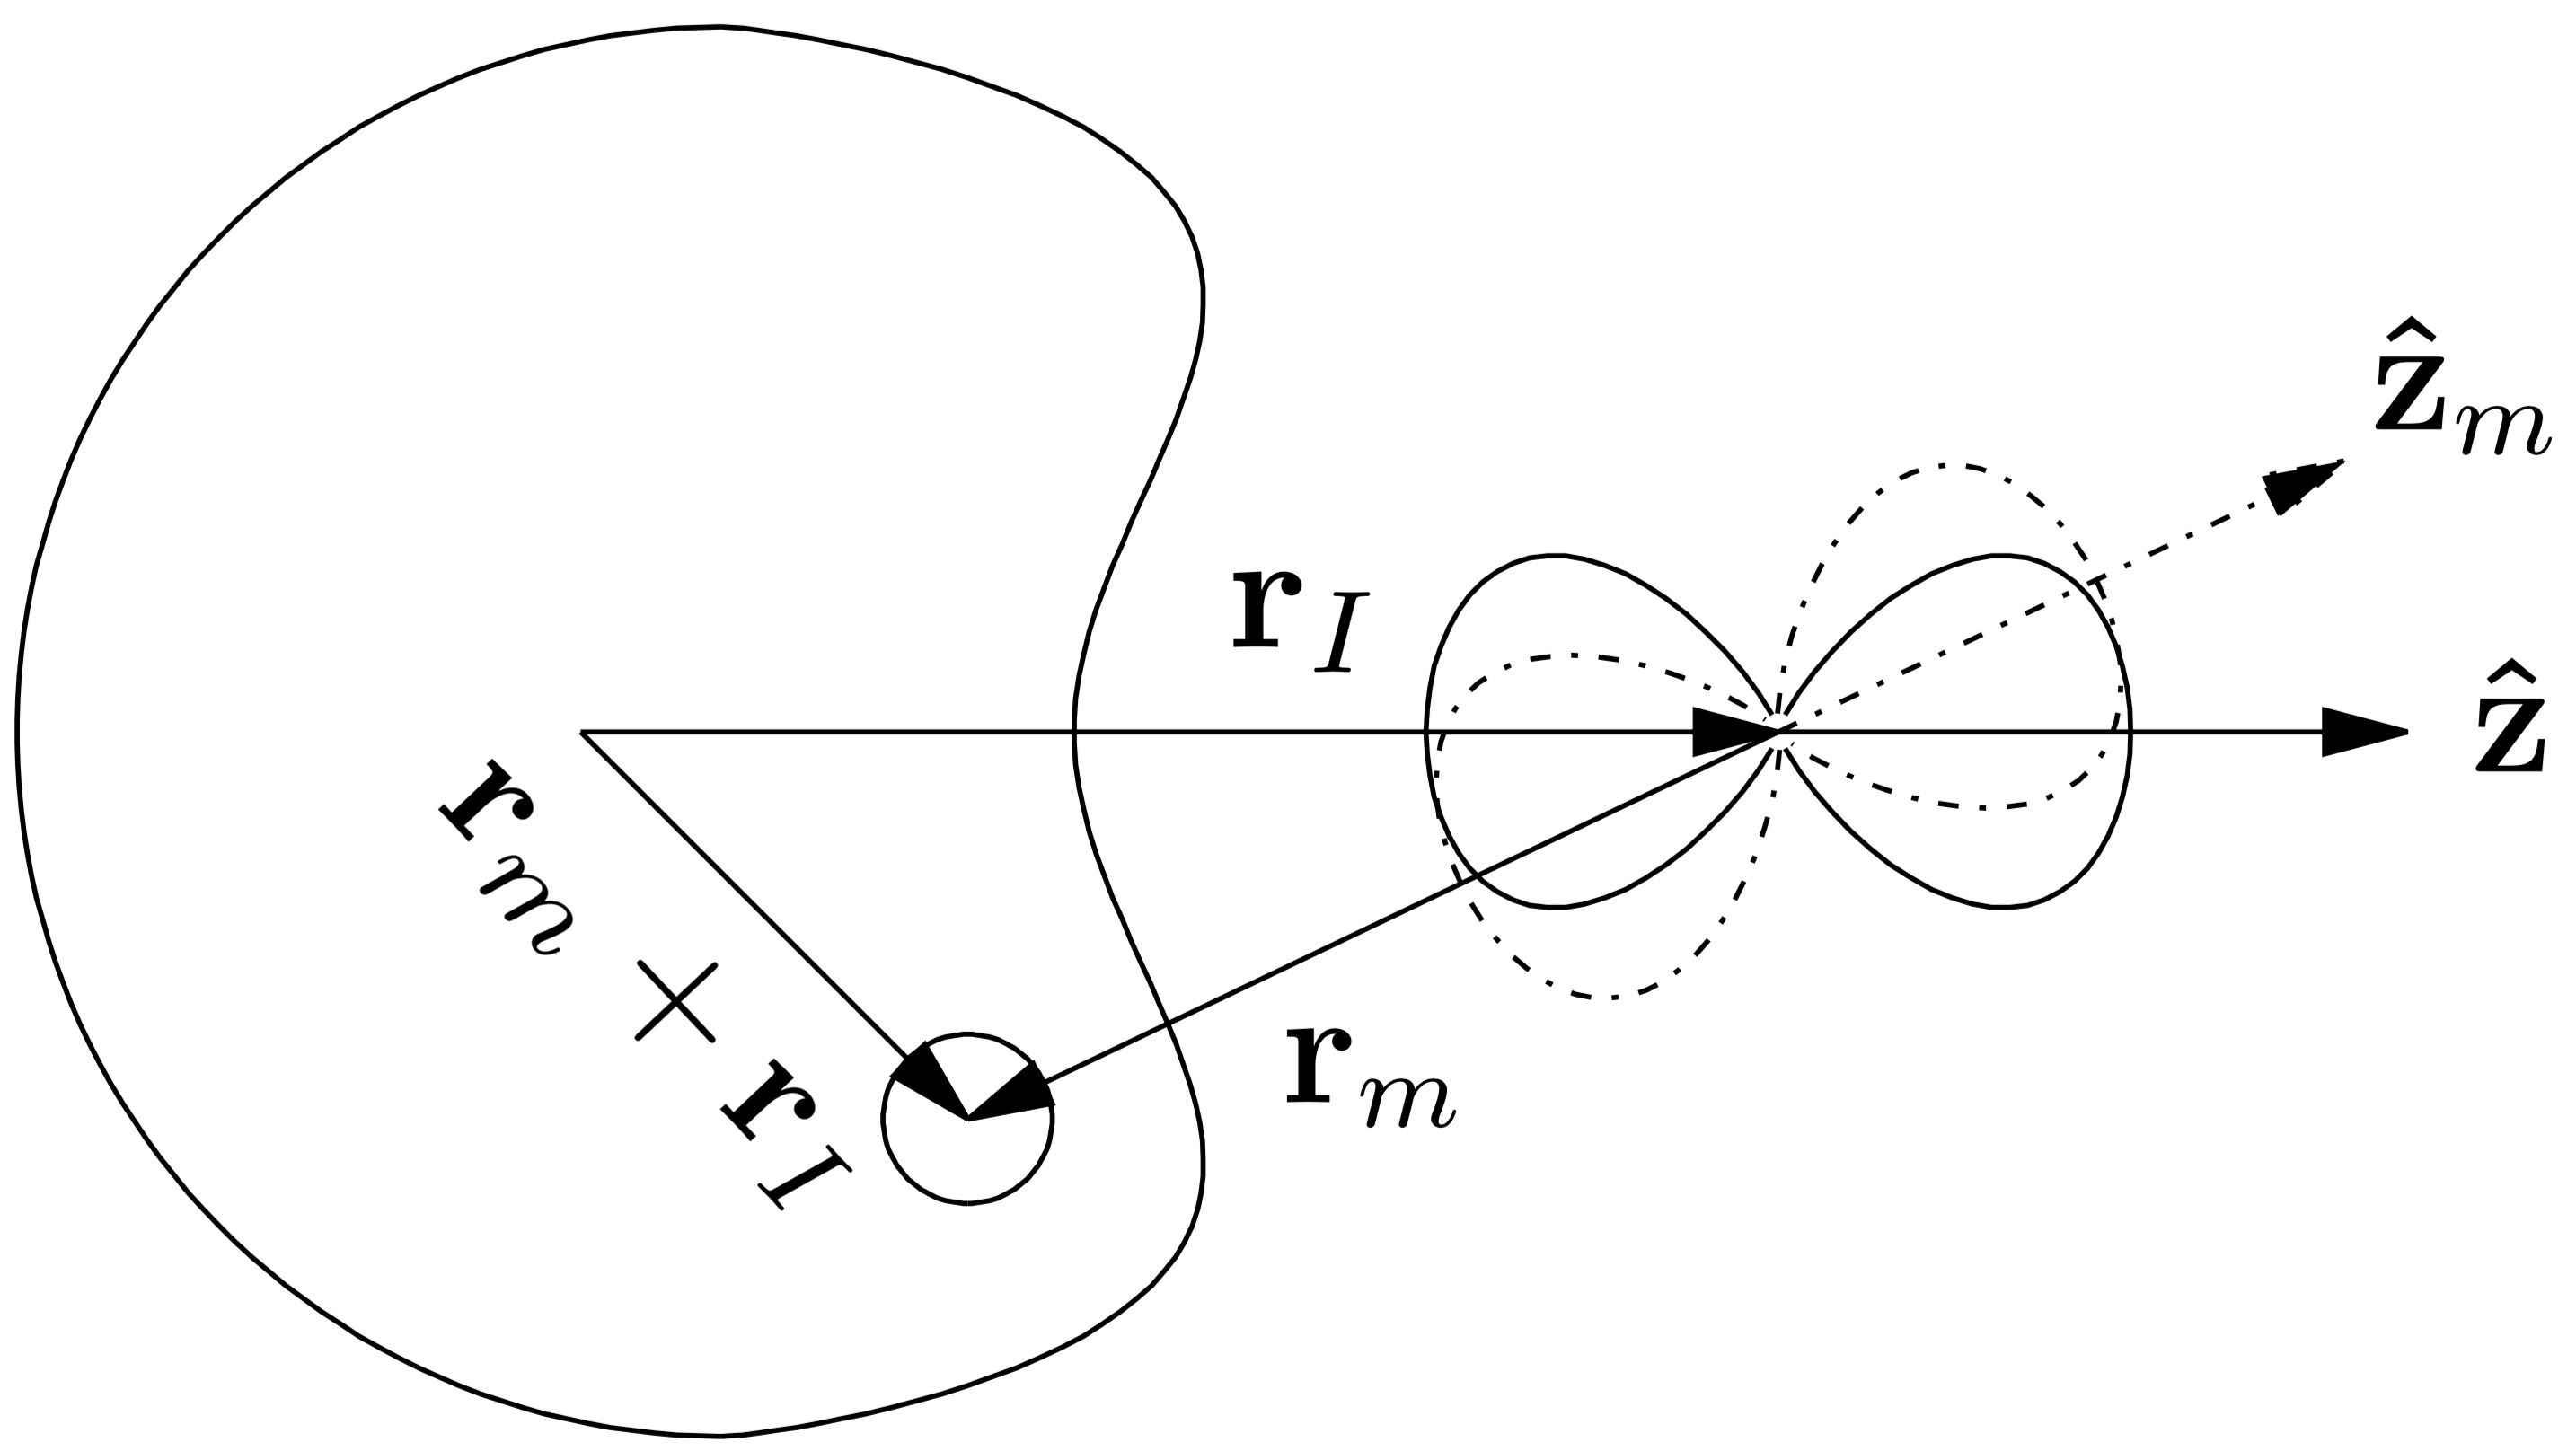
\includegraphics[width=0.75\textwidth]{dim-axes}
				\end{center}
				\caption{The set of axis defined in the DIM description. (Illustration courtesy of M. Martinez\citep{Martinez2017}.)}
				\label{fig:dim-axes}
			\end{figure}			
		
		\subsection{Including spin-orbit coupling}
			For the study of the alkali metal Rb in this work, the spin-orbit (SO) splitting of the energy levels is comparable to the splitting of the orbital angular momentum levels $\Lambda=0$ and $\Lambda=\pm 1$ due to the interaction with the helium. Therefore the spin-orbit interaction needs to be included in the total interaction Hamiltonian.
			
			The total electronic Hamiltonian is given by the sum of the DIM-interaction and the SO-interaction
			\begin{align}
				\mathcal{H} = \mathcal{U}^{DIM}+\mathcal{V}^{SO}.
			\end{align}
			The SO-matrix is approximated by the atomic alkali one, which is approximated by
			\begin{align}
				\mathcal{V}^{SO}=g\vec{L}\vdot\vec{S} = \frac{1}{2}g\qty(\vec{J}^2-\vec{L}^2-\vec{S}^2)
			\end{align}
			The coupling constant $g$ is usually approximated by that of the free atom \cite{Jak97}. We can extend the DIM basis \eq{eq:dim-basis} to include the projection of the electron spin $s=\qty{\uparrow,\downarrow}$ corresponding to the quantum numbers $m_s=\qty{\frac{1}{2},-\frac{1}{2}}$:
			\begin{align}
				\ket{p_i,s}\in\qty\big{\,\ket{p_x,\uparrow}\!,\ket{p_x,\downarrow}\!,\ket{p_y,\uparrow}\!,\ket{p_y,\downarrow}\!,\ket{p_z,\uparrow}\!,\ket{p_z,\downarrow}}.
			\end{align}
			In this basis the matrix $\mathcal{V}^{SO}$ is given by
			\begin{align}
				\mathcal{V}^{SO} = \frac{1}{2}g\mqty*(0&0&-i&0&0&1\\0&0&0&i&-1&0\\i&0&0&0&0&-i\\0&-i&0&0&-i&0\\0&-1&0&i&0&0\\1&0&i&0&0&0)
			\end{align}
			Kramers' theorem states that the two-fold degeneracy of the levels originating from total half-integer spin cannot be broken by electrostatic interactions \cite{Nak01}. Therefore all the electronic eigenstates of $\mathcal{H}$ are doubly degenerate. Diagonalising $\mathcal{H}$ yields three doubly degenerate potential energies between the impurity and surrounding helium.
			
			The dynamic evolution of the electronic excited state of the impurity is described by introducing an additional degree of freedom, a 6-component vector $\ket\lambda$, which describes the coefficients of the electronic state in the $\qty{\ket{p_i,s}}$ basis
			\begin{align}
				\ket{\lambda(t)} = \!\!\!\!\!\sum_{\substack{i=\{x,y,z\}\\s=\{\uparrow,\downarrow\}}}\!\!\!\!\! \lambda_{is}(t) \ket{p_i,s}
			\end{align}
			such that $\norm{\ip{\lambda}}^2=1$. The complete set of variables required to describe the
			system consists of the complex valued effective wave function for helium $\Psi(\mathbf{r}, t)$ with
			$\rho(\mathbf{r}, t) = |\Psi(\mathbf{r}, t)|^2$, the impurity position $\mathbf{r}_I(t)$, and the 6-dimensional complex vector to determine 
			its electronic wave function $|\lambda(t)\rangle$. The total energy of the impurity-$^4$He$_N$ complex after excitation to the $^2$P manifold is

			\begin{align}
				E[\Psi, \vec{r}_I, \lambda] &= \frac{\hbar^2}{2m}\int\!\abs{\grad \Psi}^2\diff{r}
				+ \int\!{\cal E}_c[\rho]\diff{r} \nonumber \\
				&+ \frac{p^2_I}{2 m_I}
				+ \int\!\rho(\vec{r})\,V_\lambda(\vec{r}-\vec{r}_I)\diff{r}
				+ \ev**{\mathcal{V}^{SO}}{\lambda}
			\end{align}
			where $V_\lambda$ is defined as
			\begin{align}
				V_\lambda(\vec{r}) \vcentcolon= \ev{\mathcal{V}^{DIM}}{\lambda} = \sum_{ijss'}\lambda^*_{is}V^{DIM}_{ijss'}(\vec{r})\lambda_{js'} 
			\end{align}
			and the components of the $6\times6$ matrix ${\mathcal V}^{DIM}$ given by
			\begin{equation}
				V^{DIM}_{ijss'}(\vec{r})=V^{DIM}_{ij}\delta_{ss'}=\qty{V_\Pi(r)\delta_{ij}+\qty\big[V_\Sigma(r)-V_\Pi(r)]\frac{r_i\,r_j}{\norm{\vec{r}_m}^2}}\delta_{ss'}
			\end{equation}
			The time evolution of the system is obtained by minimising the following action
			\begin{align}
				A[\Psi,\vec{r}_I,\lambda] = \int\!\bigg\{E[\Psi,\vec{r}_I,\lambda] -&i\hbar\int \!\Psi^*(\vec{r}) \pdv{t}\Psi(\vec{r})\dd{\vec{r}} \nonumber \\
				-&i\hbar\ev**{\pdv{t}}{\lambda} - \frac{1}{2} m_I \dot{\vec{r}}^2_I\bigg\}\dd{t} \label{eq:action}
			\end{align}
			Variation of the action $A$ with respect to $\qty\big{\Psi^*\!,\,\bra\lambda\!,\,\vec{r}_I}$ yields the following three coupled EL-equations
			\begin{align}
				i\hbar\pdv{t}\Psi &= \qty[-\frac{\hbar^2}{2m}\laplacian +\fdv{\mathcal{E}_c}{\rho(\mathbf{r})} + V_\lambda(\vec{r}-\vec{r}_I)]\Psi \nonumber \\
				i\hbar\pdv{t}\ket\lambda  &= \mathcal{H}\ket\lambda \nonumber \\
				m_I\ddot{\vec{r}}_I &= - \grad_{\vec{r}_I}\qty[\int\!\rho(\vec{r})\,V_\lambda(\vec{r}-\vec{r}_I)\dd{\vec{r}}] = -\!\int\!V_\lambda(\vec{r}-\vec{r}_I)\,\grad\rho(\vec{r})\dd{\vec{r}} \label{eq:dyn-el}
			\end{align}
			where the explicit time dependence of the variables is omitted for clarity. The second line of \eq{eq:dyn-el} is a $6\times 6$ matrix equation with the matrix elements of $\mathcal{H}$ given by
			\begin{align}
				H_{ijss'} = U^{DIM}_{ijss'}+V^{SO}_{ijss'} = \int\!\rho(\vec{r})\,V^{DIM}_{ijss'}(\vec{r}-\vec{r}_I)\dd{\vec{r}}+V^{SO}_{ijss'}
			\end{align}
			In the cases that SO-coupling can be neglected the 6-dimensional electronic state vector $\ket{\lambda}$ reduces to the 3-dimensional vector
			\begin{align}
				\ket{\lambda(t)} = \!\sum_{i=\{x,y,z\}} \!\lambda_{i}(t) \ket{p_i}
			\end{align}
			and the $6\times6$ matrix $\mathcal{H}$ reduces to the $3\times 3$ matrix of \eq{eq:u-dim} with elements
			\begin{align}
				H_{ij} = U^{DIM}_{ij} = \int\!\rho(\vec{r})\,V^{DIM}_{ij}(\vec{r}-\vec{r}_I)\dd{\vec{r}}
			\end{align}
			
			For the technical details about how this method is implemented the interested reader is directed to\rf{dft-guide}. For the collection of Fortran code that has been used to obtain the results presented here see\rf{Pi2017}. For the manuel to use the code, with included example calculations see\rf{Coppens2017}.

	\part{Photo-excitation dynamics of alkalis}
		\chapter{Alkali-doped nanodroplets}

	In their 1996 paper\citep{Griffin1996} Griffin and Stringari have argued that almost 100\% Bose-Einstein Condensation could be achieved in the low density surface region of superfluid He at $T=0$, as opposed to only about 10\% in the bulk. It is therefore evident that a minimally perturbing probe capable of investigating the surface of a He cluster is very desirable.\\

	It comes as no surprise then that alkali atoms are a very natural choice for exactly these type of studies.  For example, with a solvation parameter of $\lambda=0.729$\citep{Anc95}, Rb will remain bound to the surface of the droplet. Furthermore, they have a simple, well known, absorption spectrum. They introduce only weak perturbations (alkali-helium interaction energies are on the order of 1 cm$^{-1}$ [8]). Moreover, their simple, one-valence electron structure allows for detailed theoretical modelling. Lastly, theoretical calculations [9, 10] and experimental spectra [11-13] of alkali atoms in bulk liquid helium are available for comparison.

	Surprisingly, the study of alkali atoms seeded in highly quantum matrices is relevant to the optimisation of the use of solid hydrogen as a rocket propellant\citep{Carrick1993}.\\
	
	Given that the alkalies are ideal probes to probe the boundary region of the nanodroplets, the $n\mathrm{p}\,^2\mathrm{P}\leftarrow n\mathrm{s}\,^2\mathrm{S}$ transitions of the alkali atoms have attracted much interest from an experimental and theoretical point of view. The spectroscopy of the higher excited states has been thoroughly explored[32-42]. The obtained spectra can be successfully reproduced by a pseudo-diatomic model[9,21], except for the higher excited states, where the model progressively fails due to the limitations imposed by its realm of validity. While the the effect of the excited states on the spectra are now fairly well understood, their influence on the following dynamics is largely unexplored.\\
	
	In this part of the thesis, the results of the real-time dynamics of a single electronically excited rubidium (Rb) atom, residing in the surface dimple of a helium nano-droplet will be presented. The atom will be excited from its ground state 5s$\,^2\Sigma_{1/2}$ to the 5p$\,^2\{\Sigma,\Pi\}$ and 6p$\,^2\{\Sigma,\Pi\}$ manifold. This will be a combined experimental and theoretical study.
	
	\section{Experimental setup}

		\begin{figure}[t]
			\begin{center}
				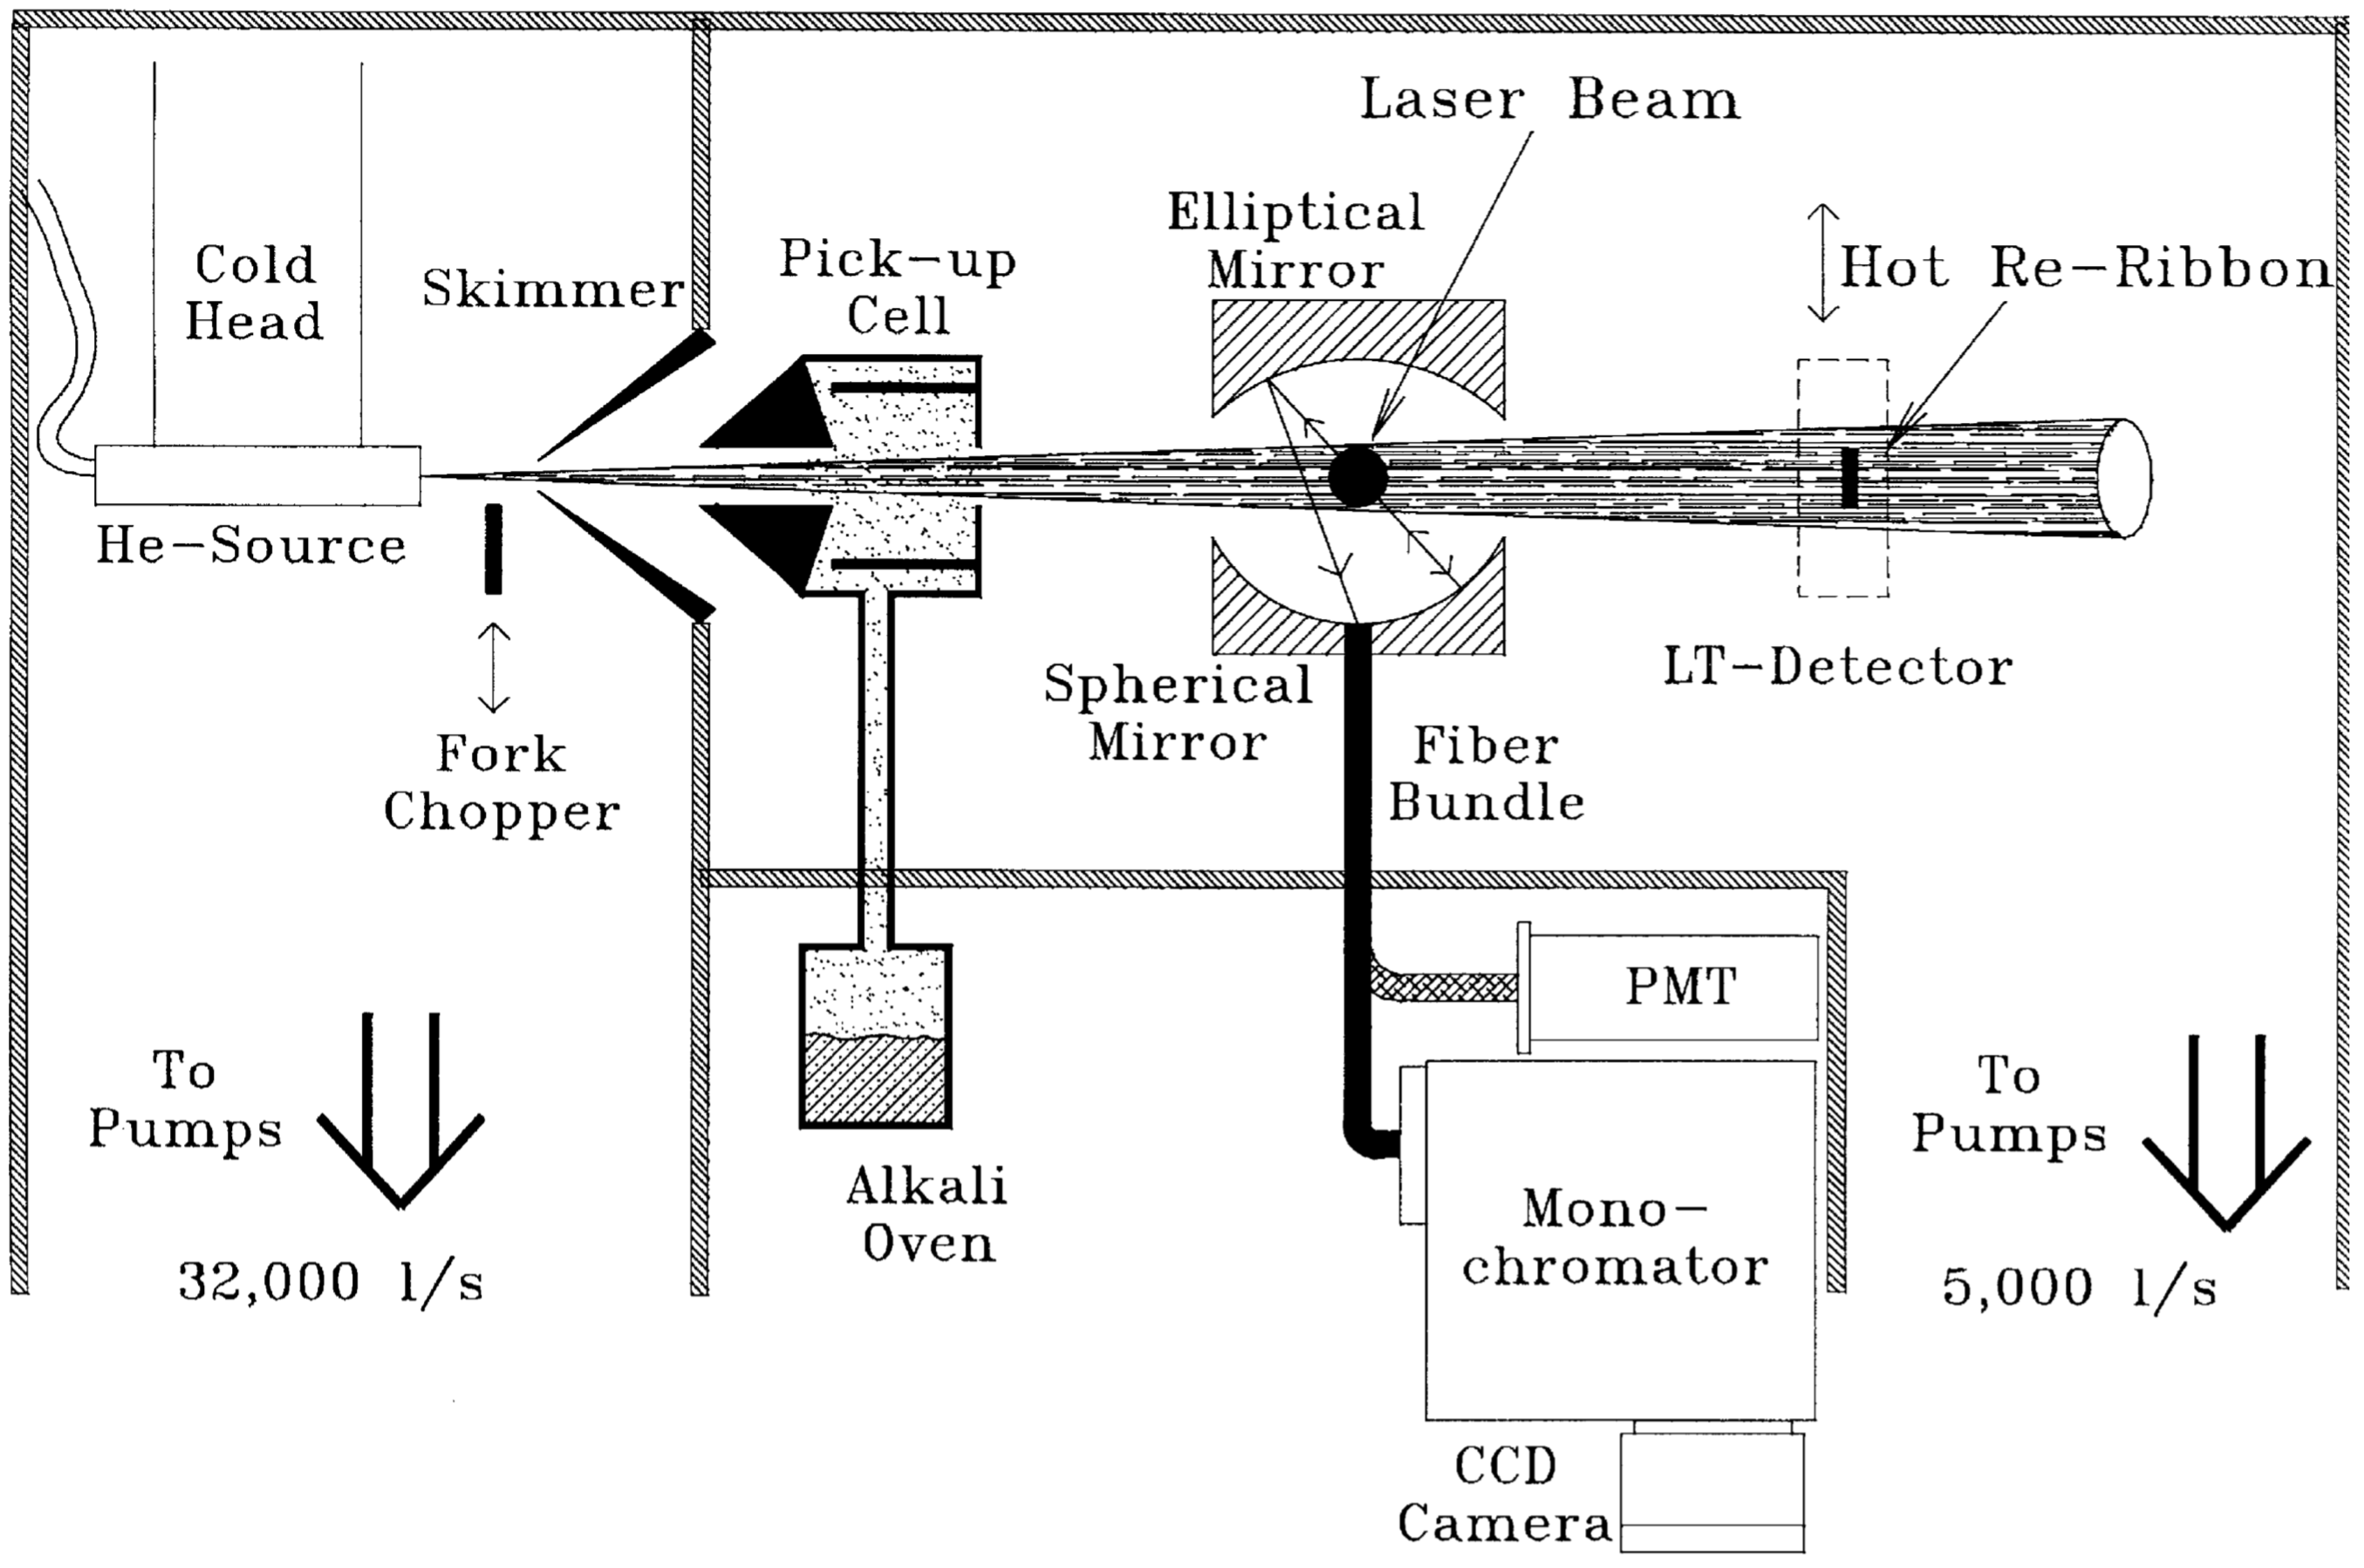
\includegraphics[width=\textwidth]{droplet-beam}
				\caption{Caption}
				\label{fig:droplet-beam}
			\end{center}
		\end{figure}
		
		\lettrine[lines=3,findent=3pt,nindent=0pt]{A}{} beam of large He clusters is produced in a supersonic expansion from a cold nozzle (Fig. \ref{fig:droplet-beam}). The weak He-He binding energy of 7.7 cm$^{-1}$ [22] requires high stagnation pressures and low nozzle temperatures ($T$) for large cluster formation. In our apparatus two CTI cryocoolers are used to establish low temperature conditions (down to 12 K) at the source. The first cooler directly cools the nozzle while the second pre-cools the supplied gas. This is needed because, even for small nozzle diameters (10$\unit{\mu m}$), at stagnation pressures up to 10$^7$ Pa the 1/$\sqrt{T}$ dependence of the gas flux leads to heavy gas loads. The pre-cooling system also provides for gas purification. The high gas throughput is easily handled by a 32000 1/s diffusion pump.
		
		At these low temperatures seeding clusters with a chromophore cannot be achieved by co-expansion and the pick-up seeding method becomes necessary [23]. According to this method, the cluster beam is sent through a scattering cell (located a short distance after the skimmer) in which a variable pressure (10$^{-3}$--10$^{-1}$ Pa) of the chromophore is maintained by connecting it with an alkali reservoir through a heated tube. The temperature of the pick-up cell, (100 K higher than the reservoir), avoids alkali atom distillation and formation of dimers inside the cell. In their path through the cell the larger clusters pick up alkali atoms without being appreciably deflected. Dissipation of the energy of the captured chromophore is likely to occur by evaporation of He atoms from the clusters, the terminal temperature of which rapidly returns to its pre pick-up value ($\approx$0.4 K) [2].
	
		To probe the picked-up alkali atoms we use laser induced fluorescence (LIF) adopting the photon collection optics design described by Hefter and Bergmann in [24]. The intersection point of the laser and cluster beam from which the fluorescence photons are collected is located a few centimetres downstream of the pick-up cell. The light of the probe laser is introduced in the apparatus via a single mode fibre and focusing optics that makes the laser beam diameter at the crossing point approximately the same as the cluster beam diameter ($\approx$2 mm). To sup- press scattered laser light we use a stack of diaphragms forming a baffle of 90 cm length both for the in- and outgoing laser beam. A Woods horn serves as a beam dump. To detect the fluorescence light originating at the point of intersection, the combination of an elliptical and a spherical mirror is used. These two mirrors focus the emitted photons at the entrance of a fibre bundle. The geometrical collection efficiency is 85\% of the 4$\pi$ solid angle centred around the intersection point. After pas- sing through the fibre bundle, the photons reach a photo-multiplier (PMT) for signal detection. The output pulses of the PMT are (after standard amplification and discrimination) stored using two gated counters which follow the cluster beam chopping frequency. Alternatively, a monochromator (GCA / McPherson, EU-700) coupled to a liquid nitrogen cooled CCD detector (Princeton Instruments, LN/CCD 1152 UV) is used for dispersed fluorescence measurements. The absolute frequency of the probe laser is monitored continuously by a home built wave meter with 0.001 cm$^{-1}$ precision. The amount and angular distribution of alkali atoms carried by the clusters can be monitored by means of a Langmuir-Taylor (LT) surface ionisation detector which is located further down- stream and is movable perpendicularly to the cluster beam direction. Since excitation at certain frequencies leads with a significant probability to a desorption of the chromophores from the cluster, we are also able to detect beam depletion spectra. Finally the LT detector provides information on the alkali atom density inside the pick-up cell by measuring the alkali background inside the detection chamber. A computer controls the laser frequency and records the acquisition of photon counts, the actual laser frequency and the parameters for cluster beam and alkali source condition characterisation.


proof is in spectra; not as shifted as in the bulk


finally introduce experiment Vangerov at al 

photo dissociation/ejection all but lowest part of $P_1/2$ excitation

introduce electronic spin relaxation to explain
and Mudrich

		\chapter{Results}
	\section{Imaging Excited-State Dynamics}
		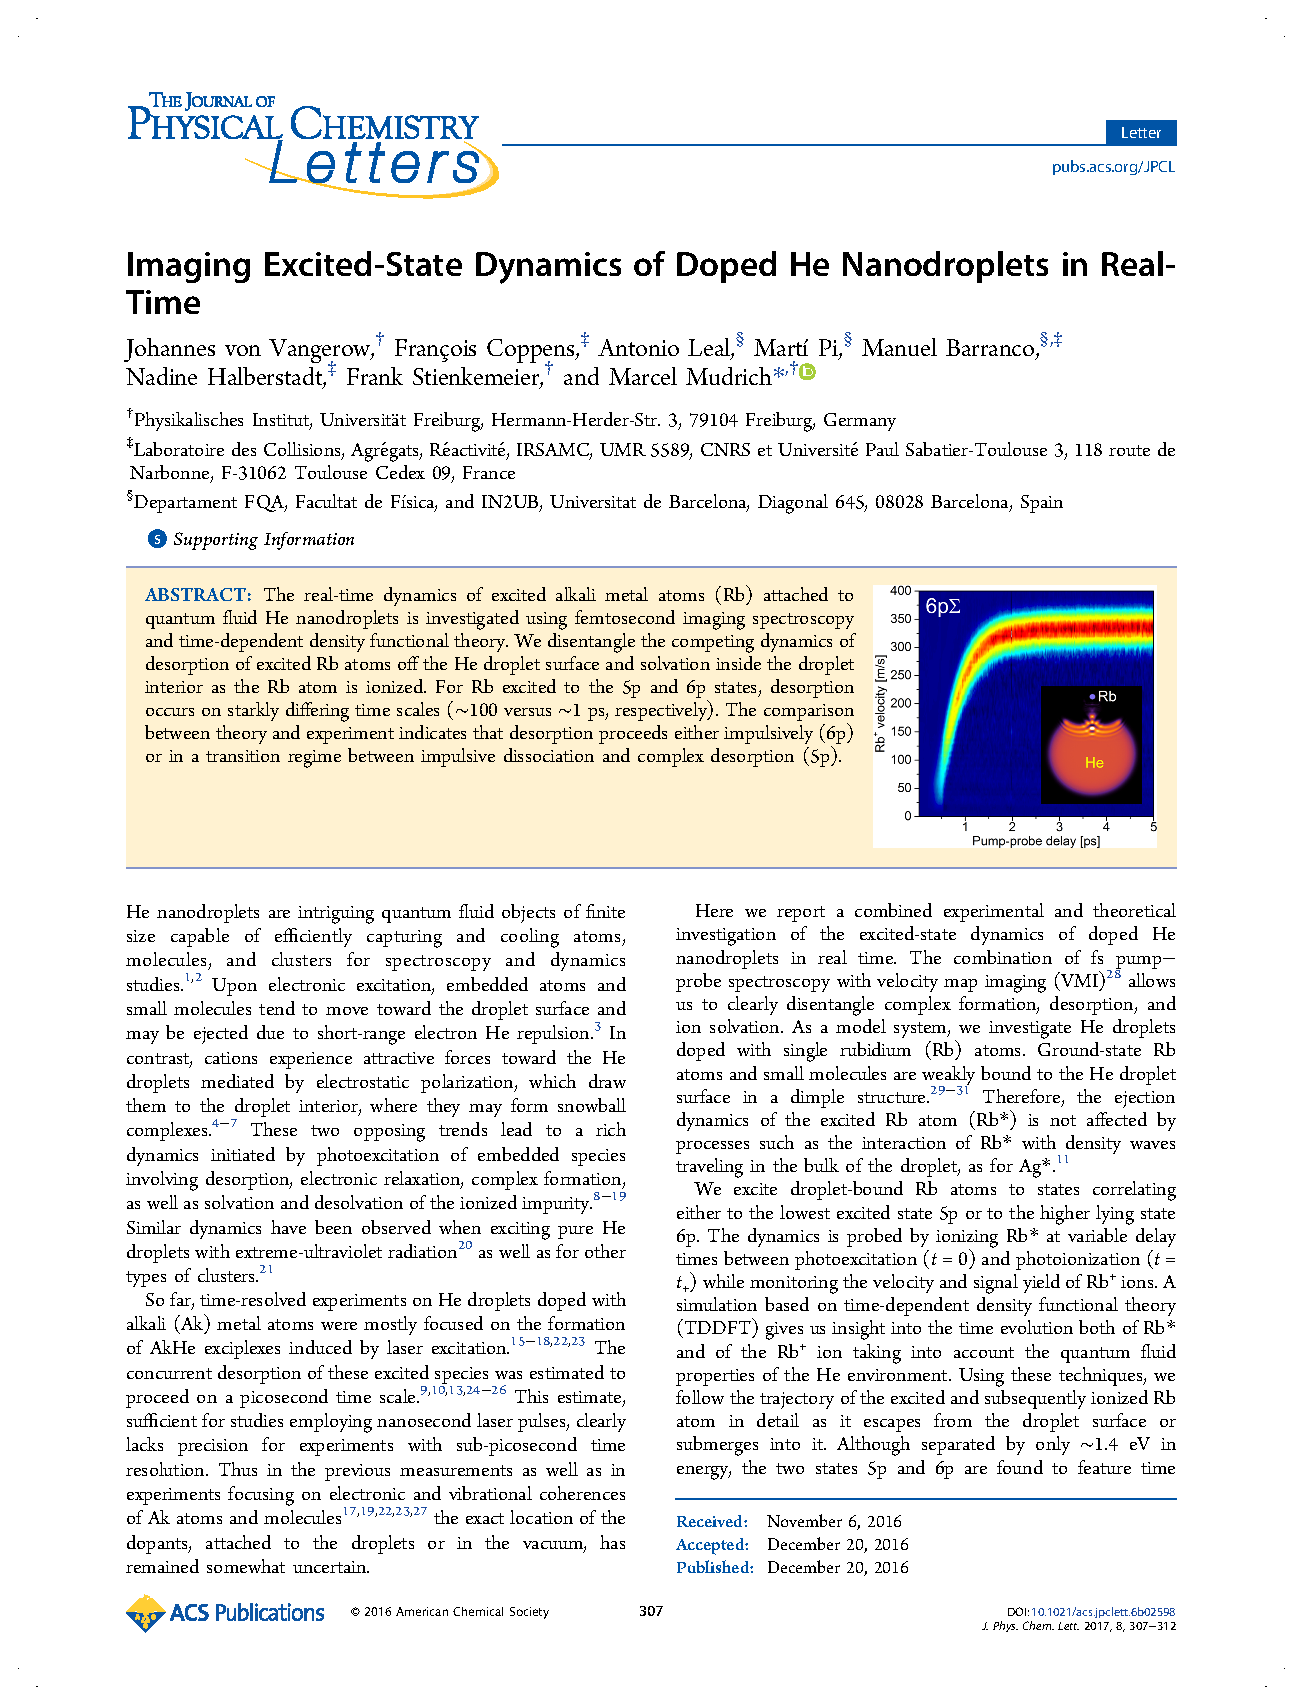
\includepdf[pages=-, scale=0.875, pagecommand={}]{jpcl_vol8_no1_pp307-312.pdf}

	\section{Desorption dynamics of RbHe exciplexes}
		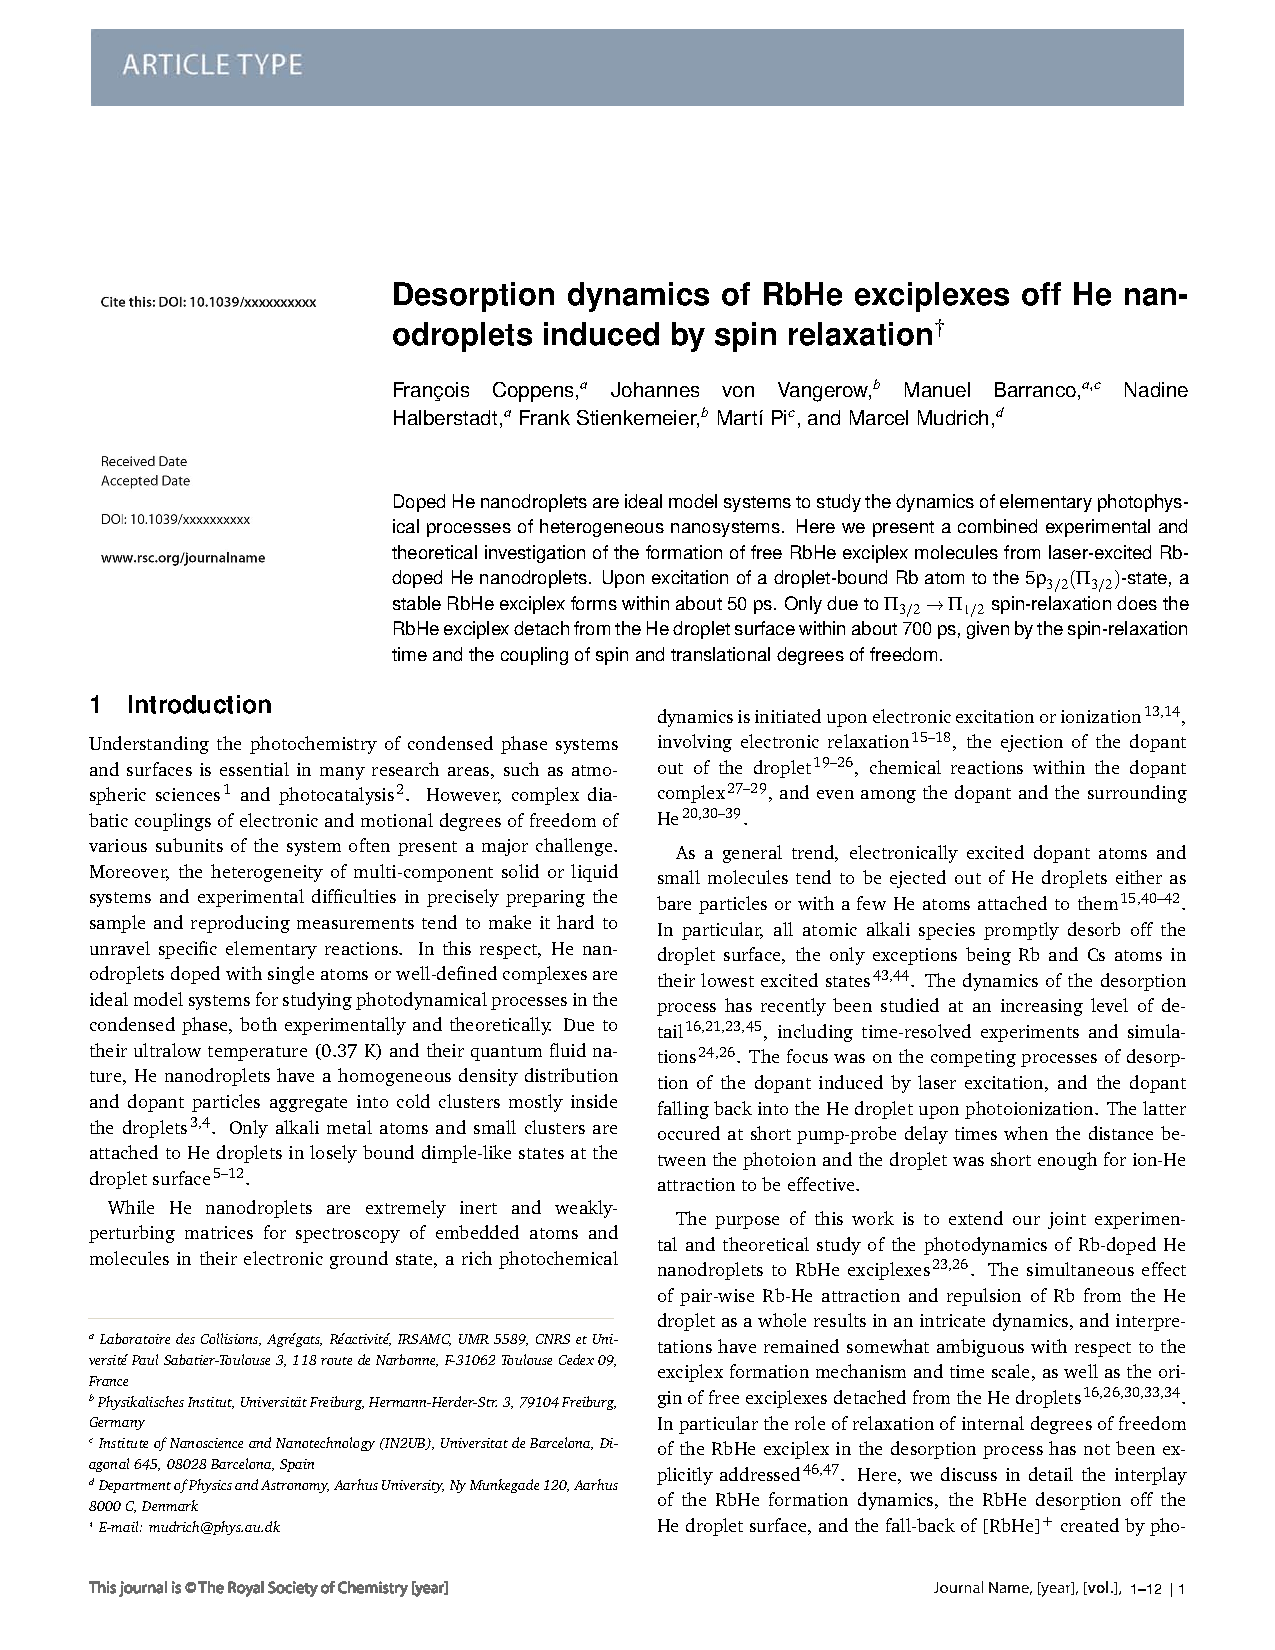
\includepdf[pages={-}, scale=0.8, pagecommand={}]{RbHe-dynamics.pdf}
	\part{Head-on collisions and capture by quantised vortices}
		\chapter{Quantised vortices in droplets}
	One of the most unambiguous signatures of the quantum mechanical nature of a substance---and indeed superfluidity---is the appearance of quantised vortices. In contrast to a normal fluid, which will rotate as a solid body when its container moves at low angular velocity, a superfluid will remain at rest. However, above a certain critical angular velocity the thermodynamically stable state of a superfluid includes one or more quantum vortices. Such a vortex can be characterised by a macroscopic wave function and quantised velocity circulation in units of $\kappa=\frac{h}{m}$, where $h$ is Planck’s constant and $m$ is the mass of the $^4$He atom [2,3]. Recently, the study of vorticity was extended to finite systems such as BECs confined to traps [3,4]. The transfer of energy and angular momentum in finite systems between quantised vortices and surface excitations is of particular interest, as it defines the nucleation dynamics, shape, and stability of the involved vortices [3,4]. In comparison to confined BECs, $^4$He droplets are self-contained and present a case for the strongly interacting superfluid. Moreover, the diameter of a vortex core which is approximately 0.2 nm in superfluid $^4$He [2] is small relative to the droplet size, suggesting a three-dimensionality of the vortices in droplets. Vorticity in $^4$He droplets has therefore attracted considerable interest [5–8].\\
	
	A schematic of the experiment is shown in Fig. \ref{fig:vortex-machine}. Helium droplets are produced by expansion of He, at 20 bar and a temperature $T_0$=5.4--7 K, into vacuum through a nozzle of diameter D 1⁄4 5 "m. The droplets cool rapidly via evaporation and reach a temperature of 0.37 K [20], which is well below the superfluid transition temperature T! 1⁄4 2:17 K [2,3]. Further downstream, the droplets capture 103–106 Ag atoms in an oven [21]. The droplets are then collided against a thin carbon film substrate at room temperature [21]. Upon impact, the droplets evaporate, leaving on the surface the Ag traces, which are subsequently imaged via a transmission electron microscope (TEM).
	\begin{figure}[t]
		\begin{center}
			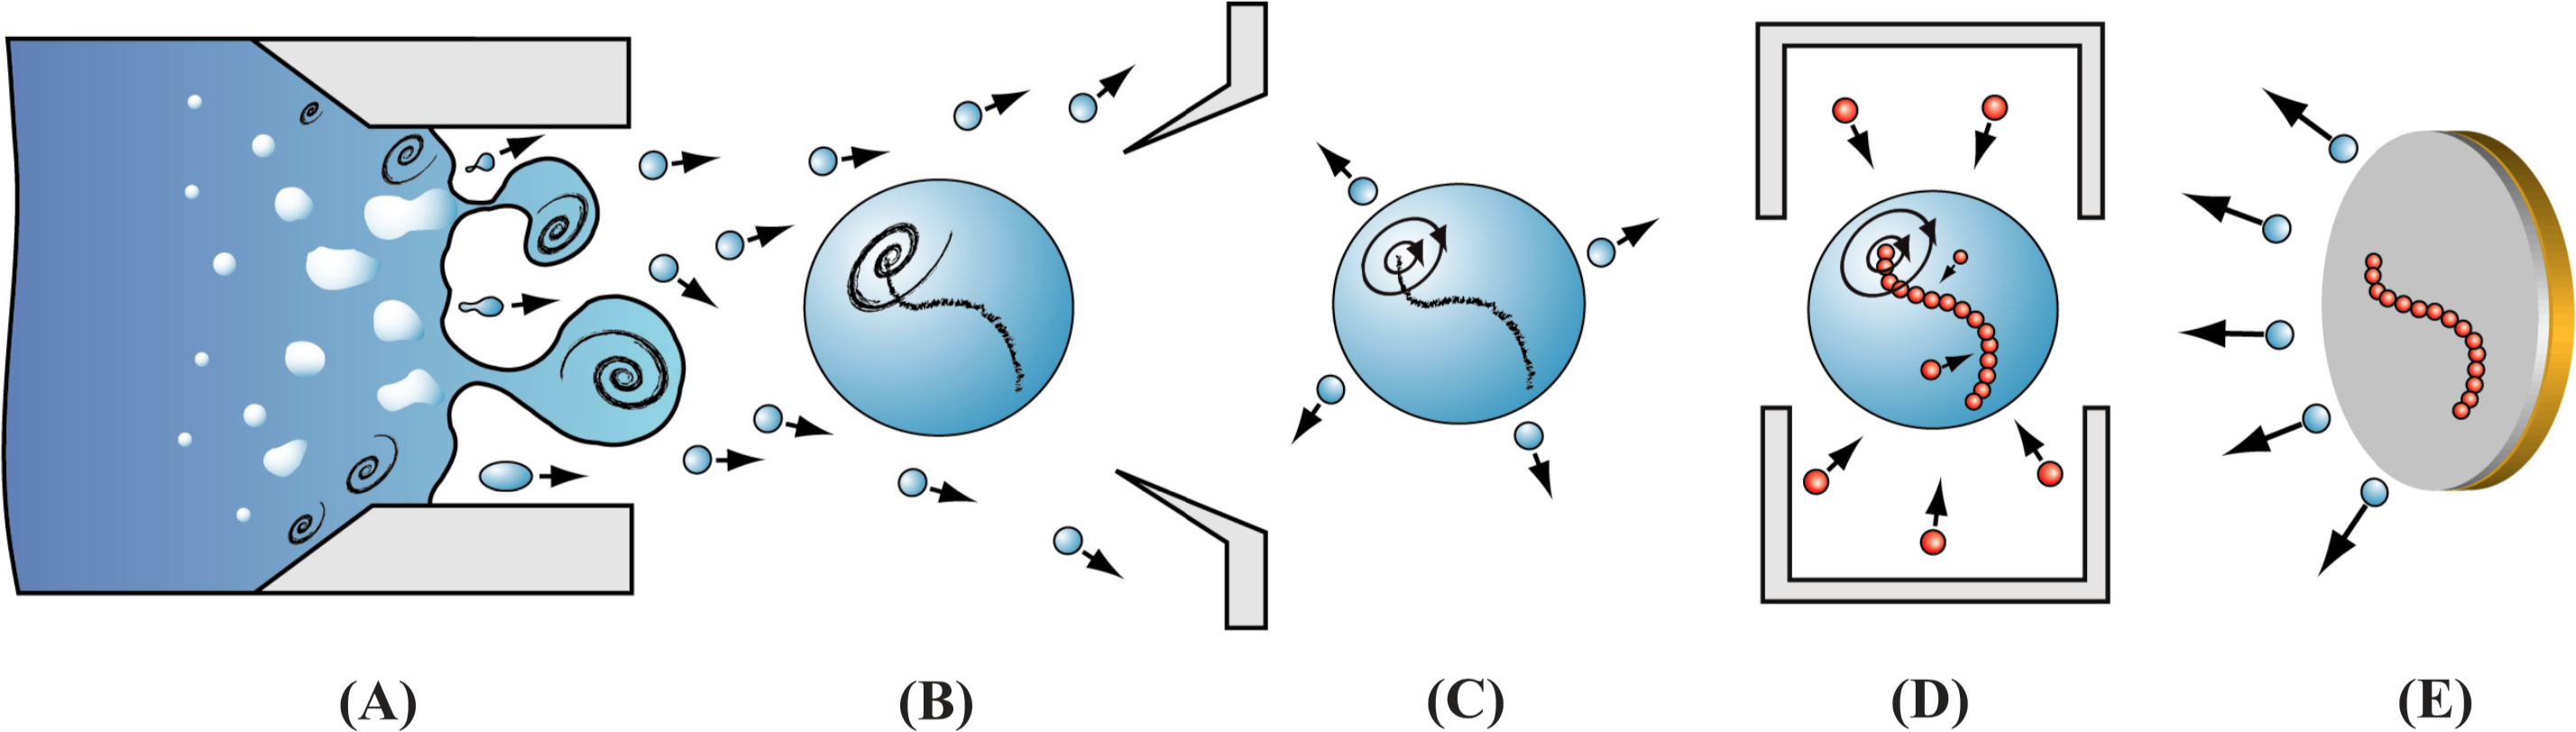
\includegraphics[width=\textwidth]{vortex-machine}
			\caption{Schematic of the experiment. (a) He fluid expands in vacuum and (b) breaks up into rotating droplets. (c) A quantum vortex is formed as a consequence of fast evaporative cooling of the droplet to below $T_\lambda$. (d) The droplet is doped with Ag atoms, which are attracted to the vortex core. (e) The droplet then collides with the carbon surface leaving behind the Ag trace, whereas the He evaporates.}
			\label{fig:vortex-machine}
		\end{center}
	\end{figure}	
	
	Recently, Gomez, Loginov and Vilesov performed experiments[PRL 108, 155302 (2012)] where vortices inside superfluid $^4$He droplets, produced by the expansion of liquid helium, were traced by introducing Ag atoms which clustered along the vortex lines, into the droplets. The Ag clusters were subsequently surface-deposited and imaged via electron microscopy. The prevalence of elongated track-shaped deposits (see Figure \ref{fig:silver-filament}) shows that vortices are present in droplets larger than about $300\unit{nm}$ and that their lifetime exceeds a few milliseconds. Two years later Gomez reported[Science 345, 906 (2014)] on the formation of quantum vortex lattices inside droplets. He used single-shot femtosecond x-ray coherent diffractive imaging to investigate the rotation of single, isolated superfluid helium-4 droplets containing $\sim\!10^8$ to $10^{11}$ atoms. The formation of quantum vortex lattices inside the droplets was confirmed by observing the characteristic Bragg patterns from xenon clusters trapped in the vortex cores (see Figure \ref{fig:vortex-array}).

	\begin{figure}[t]
		\begin{center}
			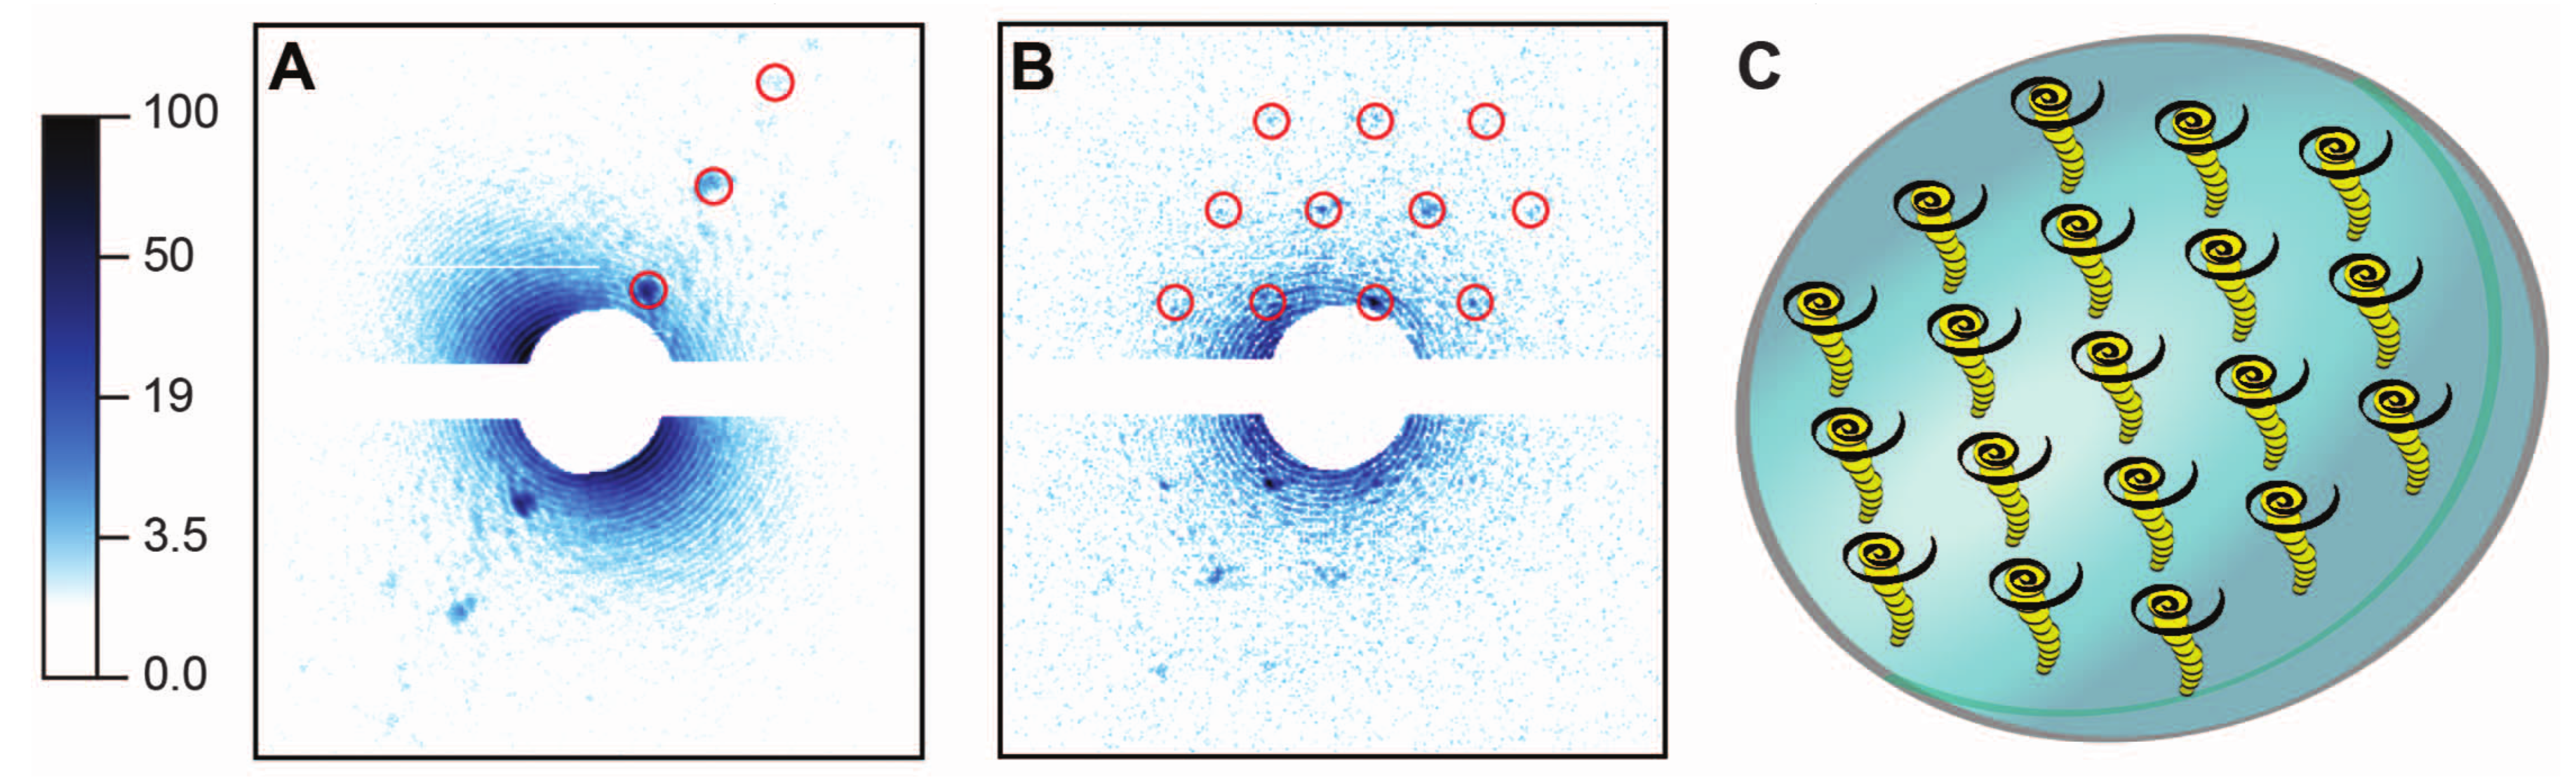
\includegraphics[width=\textwidth]{vortex-array}
			\caption{He droplets doped with Xe atoms. (A and B) X-ray diffraction images of doped droplets, displayed in a logarithmic intensity scale. (C) Droplet and embedded Xe clusters. Images in (A) and (B) correspond to tilted and parallel alignments of the vortex axes with respect to the incident x-ray beam, respectively.}
			\label{fig:vortex-array}
		\end{center}
	\end{figure}
	
%	\section{Head-on collisions}
%		\lettrine[lines=3,findent=3pt,nindent=0pt]{I}{t} is well known that helium drops readily capture foreign atoms and molecules[1], and this ability has had a considerable influence on the chemistry and physics of these systems[2]. Among the studies carried out in the past on atom-drop collisions, let us mention those aiming at experimentally determining the density profiles of large $^4$He and $^3$He droplets from the scattering of Ar and Kr atoms off helium droplets, which have been analysed within density functional theory (DFT)[3,4]; the microscopic simulation of the scattering of 3He and 4He atoms from inhomogeneous liquid helium systems[5,6]; and an earlier theoretical work on the scattering of 4He atoms from 4He droplets within a liquid drop plus optical model approach[7].\\
%
%		Very recently, time-dependent density functional theory (TDDFT) has been used to address the capture of Cs or Ne atoms by $^4$He nanodroplets[8,9]. The Cs capture was treated fully three dimensionally with the Cs atom described as a classical particle, whereas for the Ne capture study the Ne atom was described quantum mechanically, but the description was strictly one dimension.\\
%
%		Motivated by recent experiments that use Xe atoms to visualise vortex arrays in very large helium droplets[10,11], we present here a first step toward the description of the capture of Xe atoms by helium droplets, namely head-on collisions of Xe atoms against a $^4$He$_{1000}$ droplet. A discussion on the dynamic capture of Xe atoms by droplets hosting vortex lines and vortex arrays will be provided by a forthcoming study combining DFT simulation of vortex arrays as in Refs.[12,13] for helium nanocylinders and nanodroplets and collision with Xe atoms as in this work. Whenever possible, the results for Xe, a heliophilic atom, are contrasted with results for Cs, a heliophobic atom with similar mass.
%
%	\section{Capture by quantised vortices}
%		\lettrine[lines=3,findent=3pt,nindent=0pt]{I}{t} is well established that helium droplets can readily capture in their interior almost any atom or molecule interacting with them, as first shown for the case of Ne atoms[1], with the notable exception of alkali[2] and some alkaline-earth[3] atoms. This property, together with the extremely low temperature (T) achieved in helium droplets -- of the order of 0.4 K -- makes them the perfect ultracold and inert environment for hosting and studying isolated atoms and molecules, which is at the basis of current applications of helium droplets for spectroscopic studies of atoms and molecules. Besides, the superfluid nature of helium facilitates binary encounters of atoms/molecules in the bulk of the droplet while absorbing the energy released upon recombination, making possible chemical reactions which would not otherwise occur in the gas phase. These unique properties of helium droplets have had a huge impact on their study[4-8].\\
%
%		The pickup of Ar, Kr and Xe atoms in the gas phase by $^4$He$_N$ droplets with $N>10^3$ atoms produced by nozzle beam expansions was described about twenty years ago by Toennies and coworkers[9]. In these experiments, the droplets in the helium beam were deflected by impacting with a secondary beam made of rare gas atoms.\\
%
%		Recently, a technique has been introduced to determine the size of large He droplets ($N>10^5$). It is based on the attenuation of a continuous droplet beam through collisions with Ar atoms at room temperature[10]. The pickup chamber of the droplet beam apparatus is filled with argon gas and the helium droplets experience multiple, isotropic collisions with the Ar atoms on their way towards the detection chamber. Large helium droplets could also be doped in this way. This method, using Xe atoms, has been instrumental for detecting and imaging quantised vortex arrays in helium droplets[11,12]. Xe atoms were used in these experiments because of their large sensitivity to the X-ray coherent diffractive imaging employed to detect them within the helium droplets. Experiments with large superfluid helium droplets are reviewed in a recent publication[14].\\
%
%		The impurity-droplet interaction in the presence of vortices is also relevant as the first stage of a more complex process leading to the formation of nanowires, see e.g. ref. 15-18. Long filaments made of micrometer-sized solid hydrogen particles trapped on quantised vortex cores were used to directly image the vortex reconnection between quantised vortices in superfluid helium[19].\\
%
%		The impact and capture of impurities interacting with pure helium droplets have been addressed recently within time-dependent density functional theory (TDDFT). Real-time simulations have been carried out for heliophobic[20] (Cs) and heliophilic[21] (Ne) atoms. In addition to the TDDFT equation for $^4$He, heavy impurities are treated as classical particles using Newton's equation of motion, whereas a time-dependent Schr\"{o}dinger equation has been used in the case of light impurities within the mean field model[21,22]. A comparison between the results for head-on collisions of Cs and Xe atoms -- heliophobic and heliophilic atoms of similar mass -- has been presented in ref. 23.\\
%
%		In this work, we present the results obtained within TDDFT for the collision and capture of Xe and Ar atoms by a $^4$He$_{1000}$ droplet at different kinetic energies and impact parameters. Special attention is paid to the time-dependent interaction of Xe and Ar atoms with helium nanodroplets hosting vortex lines, and to the effect of multi-doped vortex arrays in large helium droplets.\\
%
%		Due to the heavy computational cost of the TDDFT simulations presented here, we address only a few facets of the capture process that we consider of experimental relevance rather than carrying out a systematic study of the process. In particular:
%		\begin{itemize}
%			\item We study the capture of Xe atoms by a $^4$He nanodroplet, both for head-on collisions and for different impact parameters, with velocities ranging from thermal values up to several hundred m/s. The results of peripheral collisions with different values of the impact parameter are used to estimate the cross section for the Xe capture.
%			\item We study how a Xe atom dynamically interacts with a droplet hosting a vortex line, under different initial conditions resulting in different velocity regimes of the impurity as it collides with the vortex core: 
%			\begin{enumerate}
%				\item[i)] a Xe atom initially at rest on the droplet surface and sinking under the effect of solvation forces
%				\item[ii)] a head-on collision of a moving Xe or Ar atom against the $^4$He nanodroplet.	
%			\end{enumerate}
%			\item We study the stationary state of a large $^4$He$_{15000}$ droplet hosting a ring of six vortex lines, doped with Ar atoms completely filling all six vortex cores. This is the simplest system that mimics those experimentally described in ref. 11, where doped vortex arrays embedded in rotating $^4$He microdroplets have been imaged.
%		\end{itemize}
%
%		Multimedia materials accompany this paper, showing the real-time dynamics of several impact/capture processes described here. These materials are presented in the ESI document. They constitute an important part of this work, since often it is only by viewing how a complex microscopic process unfolds in real-time that one can catch important physical details which would otherwise escape in a written account.
		\chapter{Results}
	\section{Head-on collisions}
		\includepdf[pages=3-9, scale=0.8, pagecommand={}]{jltp_vol187_no5-6_pp439-445.pdf}

	\section{Capture by quantised vortices}
		\includepdf[pages={-}, scale=0.825, pagecommand={}]{pccp_vol19_no36_p24805-24818.pdf}
	\chapter{Conclusions \& Outlook}

	\cleardoublepage

\appendix
	\chapter{Angular velocity and angular momentum}

\lettrine[lines=3]{\color{activeColor}I}{n} this Appendix we discuss the relationship between angular velocity and angular momentum of a deformed droplet below the critical angular frequency for vortex 
nucleation.

Let us consider an ellipsoidal vessel filled with liquid $^4$He uniformly rotating around the $z$ axis, $\omega = \omega\, \hat{\mathbf{k}}$.
The ellipsoid has the equation
 %
$$ F(x,y,z) =\frac{x^2}{R_1^2}+ \frac{y^2}{R_2^2}+  \frac{z^2}{R_3^2} - 1 = 0$$
%
If $\mathbf{v}$ is the  irrotational velocity of a point in the laboratory, $\mathbf{v}'$ the velocity of the same point in the vessel (corotating frame),  and 
$\mathbf{V}= \omega \times \mathbf{r}$, one has
%
$$\mathbf{v}'=  \mathbf{v} - \mathbf{V} = \frac{\hbar}{m_4} \, \nabla {\cal S} - \omega \times \mathbf{r}$$
%
where ${\cal S}$ is the velocity potential defined here so as  that 
%
$$\mathbf{v}= \frac{\hbar}{m_4} \, \nabla {\cal S}(x,y,z)$$
%
Its existence is granted by irrotationality;  we also have
  $\mathbf{V}= \omega \times \mathbf{r} = \omega (-y,\, x, \,0)$.
A vector  perpendicular to the ellipsoid  surface is 
%
$\mathbf{n} = \nabla  F(x,y,z)$.
%
From the stationarity condition 
%
$( \mathbf{v}'  \cdot  \mathbf{n})|_{surf} =0$
%
one obtains
%
\begin{eqnarray}
&&\mathbf{v}'  \cdot  \mathbf{n}= 0 = \left.\left(\frac{\hbar}{m_4} \, \frac{\partial {\cal S}}{\partial x} + \omega y\right) \frac{x}{R_1^2} \right.
\nonumber
\\
\nonumber
&&
+  \left. \left(\frac{\hbar}{m_4} \,\frac{\partial {\cal S}}{\partial y} - \omega x\right) \frac{y}{R_2^2} 
+  \left(\frac{\hbar}{m_4} \, \frac{\partial {\cal S}}{\partial z} \right) \frac{z}{R_3^2} \right|_{surf}
\end{eqnarray}
%
It can be checked that ${\cal S} = \alpha xy$ is a solution to this equation provided that
%
$$\frac{\hbar}{m_4} \,  \left( \frac{1}{R_1^2}  + \frac{1}{R_2^2} \right)  \alpha = \left(\frac{1}{R_2^2}  - \frac{1}{R_1^2} \right)  \omega$$
%
Hence,
%
$$ \alpha = \frac{m_4}{\hbar}\,\left( \frac{R_2^2-R_1^2}{R_1^2+R_2^2}\right) \, \omega$$
%
and
%
$$ {\cal S} = \frac{m_4}{\hbar} \, \left( \frac{R_2^2-R_1^2}{R_1^2+R_2^2}\right)  \, \omega \, xy$$
%
The velocity in the laboratory is 
$ \mathbf{v} = (\hbar/m_4)\nabla {\cal S}=  (\hbar/m_4)\alpha (y, x, 0) $,
and in the vessel (corotating frame) is
$\mathbf{v}'= \beta (R_1^2 y, \, -R_2 ^2 x, \,0) $, where $\beta \equiv  2 \, \omega/(R_1^2+R_2^2)$.
 Once they have been determined, their  circulation lines are straightforwardly obtained. 
In the laboratory frame they are
$$ x^2 - y^2 = c \quad ,$$
%
which is the appearance of the circulation lines displayed in \fig{fig8-capture}. In the vessel  frame, they are
%
$$ \frac{x^2}{(\xi R_1)^2}+ \frac{ y^2}{(\xi R_2)^2} = 1 \quad .$$ 
%
These lines are ``parallel'' to the ellipsoidal surface.

We define the deformation parameter $\epsilon$
%
$$
\epsilon =\frac{\langle x^2 \rangle - \langle y^2 \rangle}{\langle x^2 \rangle + \langle y^2 \rangle}
$$
%
where e.g., 
$$ \langle x^2 \rangle = \frac{1}{N} \int d\mathbf{r} \,  x^2 \,\Psi(\mathbf{r}) $$
%
For the sharp surface ellipsoid above,
%
\begin{equation}
 \alpha = \frac{m_4}{\hbar} \, \epsilon \, \omega
 \label{eps}
 \end{equation}
%
This relationship is not  general but  can be used as a guide for our more general approach.
Let us  now discuss the angular momentum and moment of inertia of the irrotational fluid droplet. Recalling that
%
$$L_z = - \imath \; \hbar \left( x \frac{\partial}{\partial y} -  y \frac{\partial}{\partial x}\right)$$
%
if we write 
%
$$\Psi(\mathbf{r}) = \Phi(\mathbf{r}) e^{\imath \alpha xy}$$
%
with $\Phi(\mathbf{r})$ a real function,
%
$$\langle L_z \rangle = \hbar\,  \alpha  \int d\mathbf{r} \,  (x^2-y^2)  \,\Phi^2(\mathbf{r})$$
%
If \eq{eps} holds,
%
\begin{eqnarray}
&&\langle L_z \rangle = \epsilon \, m_4 N  [\langle x^2 \rangle - \langle y^2\rangle]\, \omega   
\nonumber
\\ 
&& = m_4  N \left( \frac{[\langle x^2 \rangle - \langle y^2\rangle ]^2}{\langle x^2 \rangle + \langle y^2\rangle} \right)\, \omega  \equiv  {\cal I}_{irr} \, \omega
 \label{irrot}
\end{eqnarray}
%
where 
%
$$ {\cal I}_{irr} = m_4 N \left( \frac{[\langle x^2 \rangle - \langle y^2\rangle ]^2}{\langle x^2 \rangle + \langle y^2\rangle} \right)$$
%
is the irrotational moment of inertia. For a rigid solid,
%
$$  {\cal I}_{rig} =  m_4  \int d\mathbf{r} \,  (x^2+y^2)  \,\Phi^2(\mathbf{r}) = m_4 N [\langle x^2 \rangle + \langle y^2\rangle] $$
%
Hence, 
%
$$ \frac{{\cal I}_{irr}}{{\cal I}_{rig}} = \left[ \frac{\langle x^2 \rangle - \langle y^2\rangle }{\langle x^2 \rangle + \langle y^2\rangle} \right]^2 \rightarrow 0 \quad {\rm if} \quad \epsilon \rightarrow 0$$
%
Finally, we discuss the kinetic energy of the droplet
%
$$ E_{kin} = \frac{\hbar^2}{2 m_4}  \int \, d\mathbf{r} \,|\nabla \Psi(\mathbf{r})|^2$$
%
From the above $\Psi(\mathbf{r})$, 
%
\begin{eqnarray}
&&E_{kin}= \frac{\hbar^2}{2 m_4}  \int \, d\mathbf{r} \,|\nabla \Phi(\mathbf{r})|^2
\nonumber
\\
\nonumber
&+& \frac{\hbar^2}{2 m_4} \alpha^2 \int \, d\mathbf{r} \, (x^2 + y^2) \Phi^2(\mathbf{r})= E_{intr}+E_{coll}
\end{eqnarray}
%
where the first term is the ``intrinsic'' kinetic energy and the second term arises from the irrotational velocity field
%
\begin{eqnarray}
&&E_{coll}= \frac{\hbar^2}{2 m_4} \alpha^2 \int  d\mathbf{r} \, (x^2 + y^2) \Phi^2(\mathbf{r}) =
\nonumber
\\
\nonumber
&& \frac{1}{2} \left\{ m_4\, \epsilon^2 \int d\mathbf{r} \, (x^2 + y^2) \Phi^2(\mathbf{r})\right\} \omega^2= \frac{1}{2}\, {\cal I}_{irr} \,\omega^2
 \end{eqnarray}
% 

 These expressions may be used to obtain some estimates from the actual DFT calculations.
 For  a $^4$He$_{1000}$ droplet and $\omega$=0.10 K/$\hbar$ 
 we have obtained $\langle x^2\rangle$= 100.82 \AA$^2$ and  $\langle y^2\rangle$= 101.82 \AA$^2$; hence,
 $\epsilon \sim -1/200$. Since $\hbar^2/m_4$= 12.12 K \AA$^2$, from \eq{eps} one has $\alpha \sim -4.2 \times 10^{-5}$ \AA$^{-2}$. 
From \eq{irrot} we obtain  $\langle L_z\rangle \sim 4 \times 10^{-2} \, \hbar$.
  
 In a Bose-Einstein condensate  the deformation $\epsilon$ is a control parameter that can be set to a very large value (close to unity). For a self-bound $^4$He droplet deformation comes from
 ``rotation'' itself and it turns out to be minute
  even for angular frequencies close to the critical frequency  for one-vortex nucleation; the conclusion is that the droplet ``does not rotate'';
 in other words, it is unable to store an appreciable amount of angular momentum before vortex  nucleation.


\backmatter
	\addcontentsline{toc}{chapter}{Bibliography}
\bibliographystyle{apsrev}
\bibliography{references,review_refs}

\end{document}